\documentclass{report}
\usepackage[utf8]{inputenc}
\usepackage{amsmath}
\usepackage{natbib}
\usepackage{graphicx}
\usepackage{astrojournals} % Necesario para nombres de revistas en luis-ref.bib
%\usepackage[spanish, es-minimal]{babel}
\usepackage[vmargin=1in, hmargin=1.5in]{geometry}
\usepackage{longtable}
\usepackage{fixltx2e}



\bibliographystyle{apj}


\title{Catalog of stationary bowshock arcs in the Orion Nebula}

\author{
  Luis Angel Gutiérrez Soto\\
  Tesis de Maestría, Posgrado de Astrofísica, UNAM\\
  Asesor: Dr. William Henney, CRyA, UNAM
}

\newcommand\U[1]{\ensuremath{\mathrm{#1}}}
\newcommand\K{\U{K}}
\newcommand\cm{\U{cm}}
\newcommand\AU{\U{AU}}
\newcommand\g{\U{g}}
\newcommand\msolagno{M_\odot\,\U{yr^{-1}}}

\newcommand\thC{\ensuremath{\mathrm{\theta^1\,Ori~C}}}
\newcommand\acre{\ensuremath{_{\mathrm{acre}}}}
\newcommand\eff{\ensuremath{_{\mathrm{eff}}}}
\newcommand\Ext{\ensuremath{_{\mathrm{Ext}}}}
\newcommand\Int{\ensuremath{_{\mathrm{Int}}}}
\newcommand\ha{\ensuremath{\mathrm{H}\alpha}}
\newcommand\nii{\ensuremath{\mathrm{[N\,II]}}}
\newcommand\oiii{\ensuremath{\mathrm{[O\,III]}}}
\newcommand\sii{\ensuremath{\mathrm{[S\,II]}}}
\newcommand\Out{\ensuremath{\mathrm{out}}}
\newcommand\In{\ensuremath{\mathrm{in}}}
\newcommand\A{\ensuremath{\text{\AA{}}}}

\begin{document}
\maketitle

\tableofcontents

\begin{abstract}
 En esta tesis presentamos una lista completa de todos los arcos estacionarios de líneas de emisión (objetos LL y choques de proa de los proplyds) encontrados en unas imágenes de unos archivos del Telescopio Espacial Hubble (HST por sus siglas en inglés) de la Nebulosa de Orión. El número total de objetos detectado es de 73, de los cuales 20 no han sido reportados previamente en la literatura. Clasificamos la forma de los arcos radiactivos, mediante el ajuste de secciones cónicas en los límites internos y externos de la cáscara chocada y calculamos el brillo superficial de H alpha corregido por el fondo para cada objeto. Encontramos diferencias significativas en la forma de las cáscaras entre los objetos que se encuentran más cerca de las estrellas ionizantes y los que están más lejos. El grupo cercano, que constituyen auténticas interacciones de los proplyds con el viento estelar hipersónico, tienen formas relativamente cerradas, mientras que el grupo más lejano, que se origina debido a la interacción con el transónico flujo de champaña de gas ionizado en la nebulosa, son más abierto e hiperbólicos. Aunque algunos de estos últimos son también proplyds conocidos, muchos no lo son, los arcos más grandes y más brillantes tienden a estar asociados con luminosas estrellas jóvenes, lo que sugiere que el viento intrínsico del disco de las estrellas T Tauri podrían  jugar un papel importante. La orientación de los arcos, junto con las presiones de estancamiento estimadas a partir del brillo superficial, permiten que el campo de velocidades interno de la región H II sean probados. También  encontramos que el flujo  del núcleo de la nebulosa es aproximadamente radial y por tanto domina sobre un flujo turbulento y desordenado.
\end{abstract}


\chapter{Introducción}
% \documentclass{article}
% \usepackage[utf8]{inputenc}
% \usepackage{amsmath}
% \usepackage{natbib}
% \usepackage{graphicx}
% \usepackage{astrojournals} % Necesario para nombres de revistas en luis-ref.bib
% \usepackage[spanish, es-minimal]{babel}
% \bibliographystyle{apj}
%\title{Catalog of stationary bowshock arcs in the Orion Nebula}

% \author{
%   Alumno: Luis Angel Gutiérrez Soto\\
%   Tutor: Dr. William Henney
% }

% \begin{document}
% \maketitle

\label{chap:introduction}

Este trabajo es el resultado de la identificación y detección de arcos de emisión en los alrededores de \thC{} (O7 V) en la Nebulosa de Orión. Dichos arcos radiativos pueden ser interpretados como choques de proa que se producen por la interacción de dos vientos, esta interacción provoca que se forme una estructura con un doble choque y que la cáscara chocada está en equilibrio, es así que se puede considerar que los arcos son estacionarios. Por otro lado se tiene que en el interior de la Nebulosa de Orión; los arcos están asociados a proplyds, mientras que en regiones más externas y lejanas del grupo de las estrellas masivas llamado el Trapecio, los arcos están asociados a estrellas jóvenes de baja masa (estrellas T-Tauri). Por tanto uno de los objetivo de esta tesis, además de hacer un catálogo de choques de proa, es plantear características diferenciadoras entre los choques de los proplyds cerca de \thC{}, con los choques ubicados en las afueras de la Nebulosa de Orión, usando parámetros observacionales para estudiar sus formas y tamaños y parámetros astrofísicos para estudiar la naturaleza de la cáscara chocada de los objetos, de la región HII y de los flujos que colisionan en ambas regiones de la nebulosa. \\

De acuerdo a lo dicho anteriormente, vemos varios componentes involucrados en la formación de los arcos de proa en la Nebulosa de Orión, por tanto en este primer capítulo exploraremos un poco sobre la formación estelar en Orión, la población de estrellas masivas en esta región y su papel e importancia en la formación de los choques y la subsecuente formación de estrellas. Se hablan de los proplyds y su naturaleza, de sus flujos de gas ionizados provenientes de su frente de ionización y de la interacción de este con el viento estelar para formar los choques. Por último, se menciona en detalle la naturaleza de los arcos de emisión, donde se distinguen dos grupos; un primer grupo, que corresponde a los choques de proa de los clásicos proplyds y un segundo grupo, que son los arcos hiperbólicos LL en las regiones más alejadas de la nebulosa, donde se sugiere que los choques se forman por la interacción de un viento de una estrella T-Tauri con el transónico flujo de champaña del núcleo de la nebulosa. En los demás capítulos de la tesis estas suposiciones son probadas.                

\section{Orión y la formación estelar}
\label{sec:formation} 


Orión es la región de formación estelar más estudiada, debido a que las estrellas jóvenes y el gas nos proporcionan señales claras sobre la física en los procesos de formación estelar, la formación, evolución  y destrucción de las nubes en las que se forman las estrellas, además nos dan pistas claves y sutiles de la dinámica del medio interestelar y del papel que cumplen las estrellas de alta masa y las asociaciones OB en los ciclos del gas entre las distintas fases del medio interestelar.\\

\subsection{Estrellas masivas en Orión}
\label{sec:star}

Primero hablemos de la \textbf{Vecindad Solar} que es un caso particular donde es posible el estudio de los movimientos y distribuciones de las estrellas jóvenes relaciondas con el gas, que nos permiten trazar la historia de la formación estelar y la del medio interestelar. Como hay estrellas masivas, se crean regiones H II y estas junto a estrellas T-Tauri de baja masa trazan los sitios más recientes de formación estelar con edades entre 3 y 5 Myr \citep{Bally:2008a}, de la misma manera las asociaciones OB pueden trazar la historia de la formación estelar. Las asociaciones OB son las estrellas más masivas de la región, con ellas se pueden identificar lugares donde se han formado estrellas hace 40 Myr. Es así que las posiciones, velocidades, edades y masas de estrellas jóvenes y las propiedades del gas relacionadas con las asociaciones OB, son claves para entender la historia de la formación de estrellas y el origen, evolución y destrucción de las nubes moleculares en los últimos 100 años, logrando con esto desentrañar la naturaleza y la reciente historia del medio interestelar vinculada al nacimiento de las estrellas en esta región de la Via Láctea.\\

 Como el objetivo de nuestro estudio está centrado en la formación de estrellas jóvenes de baja masa, asociadas a estrellas masivas y regiones HII particularmente en \textbf{Orión}, entonces nos concentraremos en esta región. Las asociaciones OB en Orión consiste en un grupo de estrellas de diferentes edades que están parcialmente superpuestas a lo largo de nuestra línea de visión, dentro de estas región existen varios de estos subgrupos OB integradas por este tipo de estrellas masivas. Por ejemplo tenemos el grupo OB1a, del cúal muchos trabajos coinciden de que se trata del grupo de estrellas masivas más viejo de esta región, se encuentra ubicado en el noroesta del \textit{Cinturón de Orión} y su edad oscila entre 8 y 12 Myr \citep{Blaauw:1991, Brown:1994} dentro de este grupo hay un subgrupo conocido como el grupo 25 Orionis (25 Orionis group en inglés). El subgrupo OB1b, está centrado en el cinturón y se ha estimado que su edad comprende un rango entre 1.7 y 8 Myr, esto último es incosistente con la presencia de las tres estrellas gigantes (\(\zeta\) Orionis, \(\epsilon\) Orionis y \(\delta\) Orionis) puesto que deberían ser al menos 5 Myr más viejas, deacuerdo lo que dicen sus masas \citep{Bally:2008a}.\\

\begin{figure}
  \centering
  \includegraphics[width=.95\linewidth]{figuras-tesis/Orion-OB.jpg}
  \caption{Campo amplio de la región de Orión, que muestra los diferentes sub-grupos formados por las asociaciones OB. Tomado de wikipedia.org.}
  \label{fig:orionOB}
\end{figure}
  
En esta región se encuentra el subgrupo OB1c con edades entre 2 a 6 Myr, consiste básicamente  en estrellas que se encuentran en \textit{Orion's Sword} por su nombre en inglés, justamente frente de la Nebulosa de Orión . Este subgrupo contiene dos cúmulos, NGC 1980 ubicado en el extremo sur de \textit{Sword} y NGC 1981 situada en el extremo norte (ver figura \ref{fig:OB1-association}). Las estrellas más viejas en el Sword se superponen con poblaciones de estrellas mucho más jóvenes asociadas a la Nebulosa de Orión, M43, NGC 1977, OMC1 y 3 regiones en el \textit{Integral Shaped Filament} en el extremo norte de la nube molecular Orión A. Por otro lado tenemos a OB1d, que está formado por las estrellas de el cúmulo de la Nebulosa de Orión (ONC por sus siglas en inglés) situada en la nube molecular Orión A y por NGC 2024 ubicada en la nube molecular Orión B, son los dos cúmulos más grandes de este grupo que además resulta ser jóven, es decir con edades que van desde 2 Myr \citep{Muench:2008a}. Es difícil separar estos dos tipos de poblaciones estelares, puesto que no es claro aún si estos dos subgrupos (1c y 1d) representan diferentes poblaciones o más bien son grupos estelares jóvenes y viejos que se formaron en la nube Orión A en diferentes épocas, que desde luego han emigrado.

\subsection{Formación estelar en Orión}
\label{sec:frormacion}

Es bien sabido que la formación estelar ocurre cuando grandes nubes moleculares como Orión colapsan debido a su propia gravedad, es en ese momento cuando se desencadena la formación de estrellas de alta y baja masa. Como ya se dijo; en Orión tales fenómenos están presentes. Por ejemplo el subgrupo OB1d además de contener; el cúmulo de la nebulosa de Orión (ONC) y a NGC 2024 como se describió arriba, contiene  una docena de pequeños cúmulos y una distribución de estrellas en el fondo que están mas o menos aisladas, que se han formado en núcleos a lo largo de nubes moleculares en Orión, es el caso de las estrellas formadas en NGC 2068 y NGC 2071 en Orión. Varios miles de estrellas en su mayoría de baja masa, miembros del subgrupo 1d fueron formadas a partir de la \textit{Integral Shaped Filament} \citep{Bally:1987} en la parte Norte de la nube molecular Orión A, que contiene como ya sabemos a la Nebulosa de Orión \citep{Johnstone:1999}. Entonces cerca de 2000 estrellas de baja masa con edades menores a \(10^6\) años están concentradas alrededor de un cúmulo de estrellas masivas denominado el Trapecio en la misma Nebulosa de Orión \citep{Hillenbrand:1997} ubicada esta última a una distancia de 436~\(\pm\)~20~pc \citep{Odell:2008a}. Hay que subrayar que  cientos se están formando en el núcleo denso de OMC2 y en 3 núcleos situados en la parte norte de la Nebulosa de Orión. Hay que decir, que hay otro tipo de objetos que se han formado bajo estas circunstancias (proplyds y objetos LL) de los cuales hablaremos más adelante. A pesar de que no se sabe con certeza acerca de todos los miembros de la asociación OB, es probable que entre 5000 y 20000 estrellas se han formado en la región de orión en los últimos 15 Myr. No obstante las edades y ubicaciones de varios subgrupos en Orión indican que la formación de estrellas, ha sido propagada a través de de la nube de Orión de una forma secuencial \citep{Bally:2008a}. \\  
 
Ya desde hace muchos años se tiene conocimiento de que las estrellas fugitivas son comunmente las estrellas O, raramente se da entre estrellas B y es inexistente en las estrellas de tipo espectral posteriores a las ya mencionadas \citep{Gies:1986, Gies:1987}, en este sentido Orión es una fuente de varias estrellas fugitivas, dentro de esta se incluyen a AE~Auriga que tiene una velocidad de \(150~\text{km}~\text{s}^{-1}\)  y a \(\mu\)~Columbae con una velocidad de \(117~\text{km}~\text{s}^{-1}\) moviendose exactamente en la dirección opuesta \citep{Blaauw:1991}. Ahora datos de Hipparcos sobre movimientos propios han mostrado que estas dos estrellas y la colisión de vientos de la binaria de rayos-x \(\iota\)~Orionis, estaban ubicadas en la misma posición en el cielo hace más o menos 2.6 Myr \citep{Hoogerwerf:2001}, algunos científicos han argumentado que estas dos estrellas (AE~Auriga y  \(\mu\)~Columbae) junto a \(\iota\)~Orionis experimentaron una interacción de cuatro cuerpos que los llevó a sufrir cambios significativos, de tal manera que las estrellas más masivas se volvieron la binaria \(\iota\)~Orionis, mientras que para las estrellas menos masivas la suerte fue otra, puesto que la energía gravitacional liberada durante el encuentro lanzó a estas dos estrella fuera de la región a muy altas velocidades \citep{Gualandris:2004}.\\   

Tenemos que los movimientos propios en el cúmulo de la Nebulosa de Orión la sitúan en la interacción de los cuatro cuerpos aproximadamente, hace 2.6 Myr. Es así que la presencia de algunas de las estrellas viejas en el cúmulo de la Nebulosa de Orión; advierten que ha ocurrido formación estelar en esta región, sin embargo el número de estrellas viejas indican que la formación estelar en el gas para formar la ONC era más suave hace 2.6 Myr. No obstante, hay que resaltar que la tasa de formación estelar se ha ido acelerando con el tiempo, culminando recientemente con la formación de un grupo de estrellas masivas conocidas como el Trapecio y este proceso aún continua hasta el día de hoy.\\

\begin{figure}
  \centering
  \includegraphics[width=.95\linewidth]{figuras-tesis/OB1-association.jpg}
  \caption{Parte sur de  Orión que contiene los subgrupos OB1c y OB1d de las asociaciones OB1 de Orión. También se logra apreciar que el subgrupo OB1c parece estar directamente en frente del subgrupo más jóven OB1d \citep{Bally:2008a}. Otros cúmulos son marcados.}
  \label{fig:OB1-association}
\end{figure}
  

Si se asume que NGC 1980\footnote{NGC 1980 ha sido asociado con el subgrupo 1c de la asociación OB ubicada justamente en frente de la Nebulosa de Orión y también con la nube molecular Orión A (ver figura \ref{fig:OB1-association}).} comparte su movimiento através del espacio con \(\iota\)~Orionis, este cúmulo podría haber estado situado en el mismo lugar que el material, del cual más tarde se formaría la Nebulosa de Orión. Esto lleva a pensar que el material del cual se formaron la Nebulosa de Orión y la ONC estaba aparentemente cerca de NGC 1980 hace varios millones de años, sugiriendo que la formación de las mismas estaría desencadenado por la estrellas viejas del cúmulo NGC 1980. Ahora si esto es verdad, las estrellas más viejas de la ONC pueden ser mienbros de NGC 1980 y del sub-grupo OB1c.\\

\citet{Bally:2008a} dice que las ubicaciones y las edades de los grupos estelares en Orión, indican que la formación estelar puede propagarse a través de una nube de una forma no lineal. No obstante, una primera generación de estrellas desencadena el nacimiento de las posteriores generaciones. Es así que en Orión al parecer el subgrupo 1a fueron las primeras estrellas en formarse, consecuentemente estas estrella masiva contribuyeron al nacimiento de las 25~Ori y del subgrupo 1b. Posteriormente estas activaron la formación estelar en \textit{Orion's Sword} al sur, \(\sigma\)~Ori en el sureste, y posiblemente \(\lambda\)~Ori en el norte, por tanto en los últimos Myr se ha propagado la formación estelar dentro de \textit{Filament Integral Shaped} en la nube molecular Orión A, para formar la Nebulosa de Orión, M43, OMC2, OMC3 y NGC 1977.\\ 

\subsection{El papel de las estrellas masivas en la formación estelar}
\label{sec:star-masivas}

Las estrellas masivas inyectan energía en el medio interestelar a través de su radiación del continuo de Lyman (EUV), de sus vientos estelares y a través de la explosión de supernovas (SN). Ahora, si se usa la función de masa estandar (IMF), entonces la población estimada de estrellas jóvenes en Orión indica que entre 30 y 100 estrellas más masivas que 8 M\(\odot\), se han formado en esta región en los últimos 12 Myr, muchas de estas estrella han alcanzado la secuencia principal y posteriormente han explotado. Usando la relación edad-masa \(\tau(\text{M})~\propto~\text{M}^{-\beta}\), con \(\beta = 1.6 \pm 0.15\) en un rango de masas de 8 a 80 \(\text{M}_{\odot}\) \citep{Shull:1995}, ha mostrado que estrellas en el subgrupo 1a más masivas que 13 \(\text{M}_{\odot}\) han explotado. En los subgrupos 1b y 1c, estrellas con edades promedio de 6 Myr y con masas mayores a 20 \(\text{M}_{\odot}\), todo parece indicar que también han corrido con la misma suerte. Es así que han habido entre 10 y 20 explosiones de supernovas en la región de Orión en los últimos 12 Myr. Como consecuencia esta energía cinética liberada (\(>10^{52}~\text{ergs}\)) ha formado una enorme burbuja de gas de emisión de rayos-x, que se ha extendido creando una cáscara masiva de gas y polvo, conocida como la superburbuja Orión/Eridanus.\\

La estructura del medio interestelar en la  burbuja Orion/Eridanus proporcionan evidencias de que la energía liberada por estrellas de alta masa ha alterado profundamente la cinemática, la forma y la estructura del gas en esta región, debido a que la radiación de las asociaciones OB han probocado que la burbuja se haya inflado un poco más. La emisión de \ha{} trasa la ubicación actual del frente de ionización en Orión, además estas bajas densidades del gas se están expandiendo con una velocidad promedio cerca de 10 a 60 Km~\(\text{s}^{-1}\) hacia altas latitudes galáctica y hacia nosotros, este gas se puede ver en absorción y especialmente en el UV.\\
         
Por otro lado si somos más exigentes y nos situamos en determinadas regiones, por ejemplo donde se situa a la ONC, tenemos que la ionización está dominada por  \(\theta^1\ \text{Ori}\ \text{C}\) que es una de las estrellas masivas y jóvenes que forman el ya mencionado Trapecio. La densidad del gas ionizado decrece desde un pico de densidad electrónica de unos  \(10^{4}~\text{cm}^{-3}\) en el frente de ionización, puesto que el gas se acelera lejos del frente \citep{Henney:2005a}. En la parte más brillante de la nebulosa es decir, en el oeste del Trapecio la capa que emite es delgada (\(< 0.05 ~\text{Pc}\)), mientras que la región que emite en el este de la nebulosa es mucho más gruesa (\(\simeq 0.3~\text{Pc}\)), y esto puede relacionarse fácilmente con la extensión lateral y la distancia de  \(\theta^1\ \text{Ori}\ \text{C}\) al frente de ionización. Por otro lado los choques estacionarios que se forman en el frente de los Proplyds cerca de la estrella ionizante \citep{Bally:2000a}, son un indicativo de que hay una cavidad formada por los vientos de alta velocidad que vienen de esta estrella luminosa, además  la presencia de líneas de He I en absorción en el espectro de las estrellas del Trapecio \citep{Odell:1993, Baldwin:1991} indican que hay baja densidad en las regiones que se encuentran en la vencidad del centro del cúmulo de la Nebulosa de Orión. \\

\textbf{En resumidas cuentas}, se tiene que la presencia de estrellas másivas dispara el nacimiento de futuras generaciones de estrellas, como ha ocurrido en la región de Orión. Por otro lado hemos aprendido que los vientos estelales que son básicamente un flujo de partículas cargadas, que vienen de las estrella másivas OB, o en el caso particular de \(\theta^1\ \text{Ori}\ \text{C}\) del grupo del Trapecio en el Cúmulo de la Nebulosa de Orión crean zonas de baja densidad. Además estos vientos estelares interaccionan con el gas de la Nebulosa para formar las ondas de choques, también se da el caso que chocan con otros flujos de gas provenientes de los proplyds en las cercanías de la estrella ionizadora formando los ya mencionados choques estacionarios y con estrellas T Tauri según sea el caso en las partes más alejadas para formar los arcos de emisión. Dichos choques compactan el gas en la nebulosa y crean densidades no homogéneas que provocan el colapso gravitacional de la nube.\\

\section{Proplyds}
\label{sec:proplyds}

Hasta el momento ya es de nuestro conocimiento, que la Nebulosa de Orión alberga un conjunto de \textit{Objetos Estelares Jóvenes} (YSOs por sus siglas en inglés). Por tanto esta nebulosa nos brinda la posiblidad de estudiar las estrellas, que aún están siendo rodeadas por su material primordial. En primera instancia una oportunidad de estudiarlas surge cuando estos objetos son iluminados por una estrella ionizante, en este contexto  por \(\theta^1\ \text{Ori}\ \text{C}\), de tal manera que el gas que rodea a las estrellas será ionizado y como consecuencia este material será visible en las mismas líneas de emisión que la nebulosa. Por otro lado es posible ver la componente del polvo en extinción contra la emisión de la nebulosa, dado que la mayoría de la emisión de la nebulosa viene del fondo como ha argumentado \citet{Odell:2008}. Pero no todo termina aqui, puesto que la iluminación de la estrella masiva sobre estos YSOs, no sólo permite verlos, sino que además en el proceso parcial o total de la fotoionización de los mismos, genera un excedente de presión que provoca que el material sea expulsado a través del mecanismo de la fotoevaporación y en este sentido habrá como resultado una destrucción inevitable de sus envolventes. Estas estrellas jóvenes que tienen esa particularidad, es decir caracteríticas especiales locales de su entorno, se han etiquetado como una subclase dentro de los YSOs y han sido llamados proplyds (un acrónimo para ``disco protoplanetario'') \citep{Odell:1994}.\\

\begin{figure}
  \centering
  \includegraphics[width=.95\linewidth]{figuras-tesis/proplyd_182-413.pdf}
  \caption{Imagen de los proplyds 182-413 (izquierda) y 183-419 (derecha). Son observaciones del \textit{Telescopio Espacial Hubble} (\textit{HST}). La imagen de arriba corresponde a emisión de \(\mathrm{[O\,I]}~6300~\text{\AA{}}\)  y la de abajo a emisión de \(\ha\). En ambos proplyds sobresale lo que parece ser un disco circunestelar muy brillante en  \(\mathrm{[O\,I]}\) \citep{Bally:2000a}. La emisión de \(\mathrm{[O\,I]}\) cerca del frente de ionización es producido por la excitación por colisión. El campo de visión en cada marco es de \(4.55'' \times 13.65''\).}
  \label{fig:182-413}
\end{figure}
  
Siendo más rigurosos un proplyd puede ser definido como una estrella de baja masa presecuencia principal, envuelta en un  disco protoplanetario que esta siendo fotoevaporado por los fotones ultravioletas (UV) de una estrella masiva. En la Nebulosa de Orión los proplyds son vistos en líneas de emisión como se dijo arriba, con una una forma alargada donde uno de sus extremos que es más ancho que el otro (cabeza del proplyd), apunta en dirección a la estrella  \(\theta^1\ \text{Ori}\ \text{C}\). 

\subsection{ Descubrimiento}
\label{sec:descubrimiento-proplyds}

El primero de estos objetos descubierto y posteriormente identificado como proplyd fue LV 2 (167-317) y fue visto en la cercanías del Trapecio. En trabajos posteriores se idenficaron un conjunto de seis líneas de emisión no resueltas, es decir estrellas; en la las cercanías del Trapecio \citep{Laques:1979}. Hasta el momento no se conocía de manera clara la naturaleza de los proplyds, pero dado que son fuentes de radio compactas de emisión térmica, fueron descubiertos en estudios llevados a cabo por el \textit{Very Large Array} realizadas en el interior de la región de Huygens \citep{Garay:1987}, por tanto con las interpretaciones de las radio fuentes, dió paso  hacer una correcta identificación de los mismos \citep{Churchwell:1987}. Con la intervención del \textit{Telescopio Espacial Hubble} (\textit{HST}) se pudo establecer la verdadera naturaleza de los proplyds, ya que con la cámara WFPC2 \citep{Odell:1994} se pudieron obtener imágenes más claras y puras de esta región, como se puede ver en la figura \ref{fig:proplyd-hst}. En dichas imágenes se pueden apreciar unos objetos cerca de la estrella ionizadora, con una estrella central de baja masa y en algunas ocasiones con una región oscura en el centro.\\ 

\begin{figure}
  \centering
  \includegraphics[width=.95\linewidth]{figuras-tesis/proplyd-HST-WFPC2}
  \caption{Imagen tomada con la Cámara Planetaria (PC) WFPC2-\textit{HST}. Los colores indican las líneas de emisión o filtros usados;  verde = \(\ha~\lambda6563\), rojo =  \(\nii~\lambda6584\) y  azul = \(\oiii~\lambda5007\) \citep{Bally:1998a}. En la imagen son perceptibles los proplyds 183-405 y 182-413, además se observa un objeto con emisión algo débil llamado 183-419.}
  \label{fig:proplyd-hst}
\end{figure}
  
Como los proplyds emiten radiación, en las mismas líneas que la nebulosa, se obtuvo su espectro  corregido por la contribución de la radiación provenientes del fondo. Entonces con las primeras observaciones terrestres tomadas con el Fabry-Perot \citep{Fuente:2003} y del espectrómetro Manchester Echelle Spectrometer del telescopio Isaac Newton \citep{Henney:1997} se lograron obtener espectros muy útiles, pero no se tenía mucha confianza en estos espectros debido a la alta correción que se había hecho. Más tarde con espectrografía echelle de telescopios terrestres más grandes se produjeron mejores espectros a partir de líneas más fuertes de cuatro proplyds: 170-337 (HST 2), 177-341 (HST 1), 182-413 (HST 10) y 244-440 \citep{Henney:1999a}.  Posteriormente se obtuvieron observaciones espectroscópicas con una alta resolución espacial del proplyd 167-317 (LV 2) \citep{Vasconcelos:2005}. Los objetos 158-327 (LV 6) y 159-350 (HST 3) fueron estudiados con una buena resolución espectral en unas imágenes de la Faint Object Camera por su nombre en inglés del \textit{HST} \citep{Bally:1998a}. No obstante el más completo estudio realizado sobre  LV 2  a una alta resolución, vienen de unas observaciones \citep{Henney:2002a} del doblete a 1907-1909~\A{} de \ciii{}, usando el espectrómetro del \textit{HST/STIS}, este análisis estuvo centrado en el microjet que sale del frente de ionización del proplyd.    

\subsection{Modelo estandar de los proplyds}
\label{sec:modelo}

En la sección anterior se ha dicho que la verdadera naturaleza de los proplyds en la ONC fue revelada por observaciones de alta resolución del \textit{HST}, aunque ya anteriormente \citet{Churchwell:1987} había escudriñado en su naturaleza con observaciones en el radio. Al comienzo se pensó que la cabeza del proplyd, se formaba por la interacción de un viento suave proveniente del disco de acreción estelar, con el viento rápido de \(\theta^1\ \text{Ori}\ \text{C}\). Como a veces suele suceder en la ciencia, este modelo se dejó a un lado, puesto que se estableció que esta parte brillante del propyid (cabeza), no eran más que frentes de ionización locales \citep{Odell:1994}, en los cuales su brillo superfial disminuía como es de esperarse con la distancia a  \(\theta^1\ \text{Ori}\ \text{C}\).\\

\begin{figure}
  \centering
  \includegraphics[width=.95\linewidth]{figuras-tesis/model-proplyds.pdf}
  \caption{Modelo ampliamente aceptado para los proplyds, que básicamente representa un flujo fotoevaporado. Se tiene que el disco proptoplanetario de una estrella jóven de baja masa es afectado por los fotones estelares FUV y EUV. En este sentido la radiación FUV penetra en la superficie del disco de acreción generando una tasa de pérdida de masa, implicando con ello que se forme un flujo lento de gas neutro. Este gas neutro funciona como una capa protectora, pues absorve la radiación EUV y es así como se forma un frente de ionización que apunta en la dirección de la estrella ionizadora, entonces este frente de ionización no es más que la cabeza del proplyd. La cola del proplyd se forma debido a la fotoevopación de la parte trasera  del disco, por la radiación difusa UV. No obstante el campo de ionización difuso, que es el resultado de la recombinación del hidrógeno a su estado base \citep{Henney:1999a}, influyen de manera importante en el flujo ionizado de la cola. Claramente se puede ver que un proplyd es semejante a un cometa, aunque su cola no se debe al arrastrado por la presión de radiación como ocurre en los cometas reales. }
  \label{fig:modelo-proplyd}
\end{figure}

Es así que el modelo estandar y ampliamente aceptado postula la existecia de un  disco de acreción interno de material molecular que está rodeando una estrella jóven de baja masa presecuencia principal, que a su vez está siendo fotoevaporado por los fotones ultravioletas de una estrella masiva \citep{Johnstone:1998, Henney:1998a}. Este disco sólo es afectado por la radiación externa Ultravioleta Lejano (FUV, \(\lambda > 912~\text{\AA{}} \)), es decir radiación con energía menor a los 13.6eV necesarios para fotoionizar el hidrógeno (ver figura \ref{fig:modelo-proplyd}). Esto ocurre porque la fotodisociación de gas molecular que es calentado y suavemente expulzado a partes externas del disco forma una atmósfera extendida que es ópticamente gruesa a la radiación del continuo Lyman (EUV, \(h\nu > 13.6~\text{eV}\); \(\lambda < 912~\text{\AA{}} \)), en otras palabras los fotones FUV son los responsables de disociar las moléculas y de calentar el gas de la región de fotodisociación (PDR) a \(T\sim100-1000~\K\) dejando como resultado una estela de material neutro \citep{Johnstone:1998}. Lo anteriormente dicho implica que esta atmósfera interna está siendo rodeada por un frente de ionización local, que es más brillante en la dirección en la que se encuentra la estrella ionizante dominante, también tiene una zona con un brillo más débil que tiene la forma de la cola de un cometa, debido a la fotoinización del material por la radiación difusa del continuo de Lyman.\\ 

\subsection{Choques de proa asociados a proplyds}
\label{sec:shock-proply}

\begin{figure}
  \centering
   \includegraphics[width=.95\linewidth]{figuras-tesis/shock-proplyd}          
  \caption{Región de la Nebulosa de Orión centrada en el Trapecio, como el resultado de un mosaico de imágenes de la Cámara Planetaria; WFPC2 del \textit{HST} tomadas durante el ciclo 4 en unas observaciones de la Nebulosa de Orión, usando unos filtros de banda angosta. Los colores indican; verde es \ha{}, rojo es \nii{} y azul es \oi{}. Imagen tomada del artículo de \citet{Bally:1998a}.}
  \label{fig:shock-proplyd}
\end{figure}

Los proplyds que están situados cerca de la estrella masiva \thC{} están acompañados por arcos débiles, que son visibles por la emisión de \oiii{} y de \ha{}. También se pueden ver por la emisión de polvo de silicato, es decir en el infrarrojo a 11.7~\(\mu \text{m}\) \citep{Arredondo:2001, Hayward:1994}. A partir de unas imágenes de \ha{}+\nii{}  del \textit{HST} donde se observan los arcos en estas líneas de emisión, \citet{Bally:1998a} propone que estos arcos trazan la estructura de choques de proa formados por la interacción del viento estelar proveniente de \thC{}, con el flujo de material fotoevaporado del frente de ionización de los propyds. La figura~\ref{fig:shock-proplyd} es una región de la Nebulosa de Orión centrada en el Trapecio, que contiene los primeros objetos descubiertos por \citet{Laques:1979}. Cerca de una docena de proplyds iluminados externamente son visibles en esta imagen, además se logra apreciar que algunos tienen arcos radiativos y que todos tienen un frente muy brillante por las líneas de emisión en dirección a \thC{}.         

\section{Objetos LL  en la  Nebulosa de Orión}
\label{sec:objeto-ll}

Los típicos Objetos LL llamados así por la primera versión de estrellas LL orionis descubierta en la Nebulosa de Orión, son  básicamente arcos de emisión (vistos en líneas de emisión) asociados a estrellas jóvenes de baja masa presecuencia principal situadas en regiones externas de la Nebulosa de Orión \citep{Henney:2013a} (ver figura \ref{fig:LL1}). El prototipo de estos objetos es la estrella T Tauri LL~Ori cuyo arco de emisión fue descubierto hace 36 años \citep{Gull:1979a}. Posteriormente se identificaron seis objetos más, con características similares \citep{Bally:2001a} y fueron denotados empezando desde LL1 hasta LL7, donde el primero de estos corresponde a LL~Ori. La lista de Objetos LL detectados siguió en aumento, puesto que gracias a datos de líneas de emisión en el óptico (\(\ha~6563~\text{\AA{}}\), \(\nii~6584~\text{\AA{}}\) y \([\text{SII}]~6716,6731~\text{\AA{}}\)) del Telescopio Espacial Huble (HST) \citep{Bally:2000a, Bally:2006a} se han identificado cerca de 20 objetos. No obstante muchos de estos objetos tienen jets muy coliminados que se originan en la estrella T Tauri, que de alguno u otra forma alteran la morfología de los arcos de emisión. Es el caso de LL1 quien posé un jet hipersónico del tipo Herbig Haro conocido como HH 888.\\

\begin{figure}
  \centering
  \includegraphics[width=.95\linewidth]{Figures/ll-figs/LL1-schematic.pdf}
  \caption{\textit{Izquierda}. Ubicación de LL~Ori en el suroeste de la Nebulosa de Orión. Esta imagen es el resultado de la convinación de observaciones del HST-WFPC2 \citep{Odell:1996} con los filtros: \(\ha~\lambda6563\) (verde), \(\nii~\lambda6584\) (rojo) y \(\oiii~\lambda5007\) (azul). Hay una región de saturación en el Trapecio y esta aparece en color blanco siendo una imagen superpuesta de \(\ha\). \textit{Derecha}. Es una ampliación de la zona donde se encuentra LL~Ori. Se puede ver el hiperbólico choque de proa, que se forma debido a la interacción de un viento de una estrella T Tauri, con  el flujo de champaña de gas ionizado  proveniente del núcleo de la Nebulosa de Orión. También se puede apreciar un objeto HH (jet) asociada a la  estrella T Tauri, en  el cual el choque de este tiene movimientos propios \citep{Henney:2013a} y una velocidad radial (flecha de color). Las velocidad de las alas del choque es de \(\sim 20 ~\text{km}~\text{s}^{-1}\), mientras que la velocidad del jet es muy superior (\(60-120 ~\text{km}~\text{s}^{-1}\)). Imagen de William Henney.}
  \label{fig:LL1}
\end{figure}

\subsection{Naturaleza de los arcos de proa LL }
\label{sec:choques}

Los objetos LL Orionis pueden ser interpretados como la interacción supersónica de un viento interno de una estrella T-Tauri, con el flujo ambiental de la Nebulosa, aunque es apresurado pensar en una típica estrella T Tauri como el objeto que proporciona el viento interno, puesto que aún no se conoce con certeza la naturaleza del viento interno, debido a que el flujo fotoevaporado proveniente del disco protoplanetario de un proplyd también es un candidato muy fuerte para el viento interno (en esta tesis se intentarán aclarecer estos argumentos). En una escala más grande el viento externo parece ser originario de la  región H II en el núcleo de la Nebulosa de Orión. Esto es debido a que cuando un frente de ionización envuelve un objeto muy denso, se forma un flujo fotoevaporado de gas ionizado con un frente D-crítico \citep{Dyson:1968}. Entonces, a este flujo de ahora en adelante lo llamaremos flujo de champaña y como han indicado \citet{Mellema:2006, Arthur:2011, Ercolano:2012}, este flujo surge durante los procesos de evolución de una región H II dentro de una nube molecular turbulenta.\\

\paragraph{Esquema general de los Objetos LL.} La figura \ref{fig:esquema-arcos} nos muestra un esquema general de los choques de proa en la Nebulosa de Orión, es así que los arcos hiperbólicos de los objetos LL se forman, debido a que el flujo de Champaña (izquierda), que entre otras cosas es ligeramente supersónico (\(M\simeq2\)) choca con un obstáculo (derecha), que en este caso es un flujo también supersónico asociado a una estrella jóven de baja masa, no obstante el choque externo es muy radiativo proporcionando con esto, un arco de emisión brillante, es decir muy visible. La naturaleza del obstáculo aún no es clara; puesto que  es posible que sea el flujo suave de un gas ionizado proveniente del frente de ionización del Proplyd (arriba) o podría ser el viento de una estrella T Tauri (abajo).\\ 

\begin{figure}
  \centering
  \includegraphics[width=.7\linewidth]{Figures/ll-figs/LL-outer-inner.jpg}
  \caption{Esquema general de los Objetos LL}
  \label{fig:esquema-arcos}
\end{figure}

\section{Choques de proa estacionarios en la Nebulosa de Orión}
\label{sec:shocks}

\paragraph{La zona chocada.} En general se dice que los choques de proa de los objetos LL y de los proplyds son estacionarios, debido a que no se les han detectado movimientos propios y además muestran pequeñas velocidades radiales. Por otro lado, la región chocada es ancha debido a que la interección de dos viento, provoca que se forme un doble choque, entonces tenemos un arco interno y un arco externo separados cierta anchura. Ahora sí unos de estos choques es fuertemente radiativo será visible un arco de emisión. Si este el caso, el choque podría considerarse isotérmico, puesto que la zona de enfriamiento en el choque es muy pequeña cuando el flujo es medianamente supersónico (\(20-60~\text{km}~\text{s}^{-1}\)) y la densidad es alta (mayor a unos cientos \(\cm^{-3}\)). Este fenómeno es comparable a lo descrito por \citet{Henney:2002} en la interacción de los vientos de dos proplyds; cuando la temperatura del gas en la cáscara chocada se eleva por la termalización de la energía cinética pre-choque, dando como resultado un aumento en las emisiones, puesto que la energía térmica se irradia y el gas retorna nuevamente a su estado de equilibrio. En el caso particular de LL1, la emisión en la cáscara chocada en equilibrio está dominada por líneas de recombinación tales como \ha{}, mientras que para las líneas excitadas colisionalmente dominan las de \oiii{} en los objetos cerca del Trapecio y las líneas de \nii{} en los arcos LL donde las líneas de \oiii{} son débiles.\\ 

\begin{figure}
  \centering
  \includegraphics[width=.95\linewidth]{Figures/ll-figs/wind-geometry-extended-lores.jpg}
  \caption{Esquema de la interacción de los vientos en la Nebulosa de Orión. la región de color verde corresponde a gas molecular neutro cuya temperatura oscila entre los 50 y los \(1000~\K\); la zona roja es el gas fotoionizado, ahí la temperatura es de aproximadamente \(10^{4}~\K\) y las densidades van de \(10^{2} ~\text{a}~10^{4} ~\cm^{-3}\) y por último el color azul representa el material del viento estelar con \(T \geq 10^{6}~\K\) y \(n \sim 1~\cm^{-3}\). Las flechas hacen referencia al flujo de gas transónico y supersónico, por otro lado los choques de proa radiativos son ilustrados por las líneas rojas oscuras y gruesas, mientras que los choques no-radiativos son ilustrados por la línea discontinua azul y la línea de puntos también azul indica la discontinuidad de contacto. Los choques de proa ocurren en dos regiones de la nebulosa: una zona interna de interacción (cuadro izquierda arriba), donde los choques de proa externos se producen debido al viento hipersónico de una estrella másiva (\(V \sim 1000~\text{km}~\text{s}^{-1}\)) y una zona externa de interacción (cuadro derecha arriba), donde los choques externos se forman debido al flujo lijeramente supersónico y fotoevaporado de champaña (\(V \sim 20~\text{km}~\text{s}^{-1}\)). El choque externo es no-radiativo en la zona interna de interacción pero radiativo en la zona externa de interacción. Esto sugiere que el choque de proa interno es radiativo cuando el viento interno es un flujo de gas fotoevaporado de un proplyd. (Imagen de William Henney).}
  \label{fig:esquema-interraccion-vientos}
\end{figure}

\paragraph{Dos poblaciones de choques de proa.}
Los choques de este contexto se han divido en dos grupos; el primer grupo corresponde a los clásicos choques de proa de los proplyds \citep{Robberto:2005, Bally:1998a}, de estos objetos se ha habla con más detalle en \S\ref{sec:shock-proply} y el segundo grupo corresponde a los típicos arcos hiperbólicos LL (ver figura \ref{fig:esquema-interraccion-vientos}). En el caso de los proplyds que están situados en las proximidades del Trapecio, el choque de proa externo no es visible porque este se produce por la interacción con un viento muy rápido y de baja densidad (\(n \sim 1 ~\cm^{-3}\)) de una estrella O, dando como resultado que la cáscara externa sea no-radiativa. No obstante el arco interno si es visible, dado que el choque interno se forma a partir de un flujo de gas muy denso (\(10^{3}-10^{4}~\text{cm}^{-3}\)) y ligeramente supersónico (\(M \simeq 3\)) proveniente del frente de ionizacion del proplyd. En el caso de los arcos hiperbólicos, se tiene que están ubicados en regiones externas de la nebulosa, es decir están mucho más lejos del Trapecio, incurriendo en el hecho de que el arco exterior de la región chocada sea radiativo, por tanto en este domina la emisión. Otra característica diferenciadora de sus semejantes los proplyds, es que los arcos de estos tienden a hacer más abiertos.\\ 

\begin{figure}
  \centering
  \includegraphics[width=.95\linewidth, trim=30 20 30 30, clip]{figuras-tesis/proplyd-and-LL-arc.pdf}
  \caption{Tipos de choques estacionarios en la Nebulosa de Orión. (a) Choques de proas asociados a proplyds; el choque se forma por la interacción de un flujo de gas fotoevaporado que viene del proplyd a una velocidad entre 30-40 km \(\text{s}^{-1}\), con un viento que viaja a una alta velocidad (\(>1000 ~\text{km} ~\text{s}^{-1}\)) desde una estrella masiva del Trapecio. En la imágen aparecen los proplyds 177-341 y 173-342. También se observa un choque formado por la interacción de los vientos de dos proplyds.(b) Arcos hiperbólicos LL; el choque se forma debido a la interacción de un flujo de champaña de baja velocidad (\(\simeq 20~\text{km} ~\text{s}^{-1}\)) con un viento estelar que viene de una estrella T-Tauri o de un proplyd. Estas imágentes son tomadas de las observaciones del HST-ACS usando el filtro f658n, es decir de \(\ha + \nii\) y se observan los objetos; LL 6 con su respectivo jet HH 876, 308-3036 y 344-320. }
  \label{fig:proplydbow-objetoll}
\end{figure}

\subsection{Choques de proa producidos por Objetos HH y su relación con los Objetos LL}
\label{sec:herbig}

La importancia de hablar de los jets Herbig Haro en este trabajo radica en dos particularidades: primero, no confundir los choques de proa de los objetos LL con los choques de prao producidos por los jets HH. Se tiene que los choques de los objetos Herbig Haro a diferencia de los arcos LL, son producidos por la interacción de un jet colimado de material que se mueve a altas velocidades\footnote{Estos jets problablemente se originan en un objeto estelar jóven.}, con el ambiente de gas nebular \citep{Odell:1994}. Además de eso los choques HH muestran grandes movimientos propios y altas velocidades radiales. Segundo, varios objetos LL tienen jets muy colimados, lo cual a primera vista, sugiere que estos le dan la forma a los arcos LL, pero recientes estudios han mostrado que en el caso de LL1, la cinématica del choque de proa y del jet Herbig Haro (HH 888) no coincide, puesto que la del choque es simétrica y la del jet es asimétrica. Mientras para LL2 la asimetría cinématica del jet HH 505 es totalmente opuesta al del choque de proa del objeto LL en cuestión (Ver figura \ref{fig:LL1} y figura \ref{fig:objecthh} arriba izquierda). Esto parece indicar que los choques hiperbólicos son independientes de los jets Herbig Haro \citep{Henney:2013a}. Decimos esto porque en algunos casos las alas de los arcos sí están asociadas a los jets HH, como parece ser el caso de LL 6 en la figura \ref{fig:proplydbow-objetoll}, donde no es claro si las alas de su choque son generadas por el jet que se origina en la estrella presecuancia principal.

\begin{figure}[htp]
\centering
\begin{tabular}{l l}
(a) & \\
 & \includegraphics[width=0.4\linewidth, trim=60 20 20 30, clip]{./Figures/ll-figs/LL2-Will-Crop-Annotate.jpg}
\includegraphics[width=0.5\linewidth, trim=10 10 10 10, clip]{./Figures/ll-figs/HH-529-10x10arcsec-annot.pdf}
\\
& \\[2\baselineskip]
(b) & \\
& \includegraphics[width=0.92\linewidth, trim=30 150 30 100, clip]{./figuras-tesis/hhbowshock.pdf}
\\
\end{tabular}
\caption{(\textit{a}) \textit{Izquierda}. En la imagen se observa otro de los ya estudiados objetos LL en Orión. Es básicamente la estrella T-Tauri IX Ori ubicada en una región lejana en el oeste de la Nebulosa de Orión, con su choque de proa asociado (LL 1) y su jet bipolar HH 505. También son visibles regiones de emisión de \oiii{}. \textit{Derecha}. Superficie de trabajo producida por un jet hipersónico muy colimado conocido como HH 529. Tienen altas velocidades radiales (\(50-100 ~\text{km}~\text{s}^{-1}\)) y también altos  movimientos propios perpendiculares al arco (Imágenes de Henney). (\textit{b}) Choque de proa de un objeto HH conocido como HH 202, (izquierda) del HST-WFPC2 y (derecha) a 11.7 \(\mu\) (T-ReCS). Se tiene que en la imagen del HST los colores indican; verde \ha{}, rojo \nii{} y azul \oiii{} \citep{Smith:2005}.}\label{fig:objecthh}
\end{figure}

\subsection{Notación de los objetos LL y de los proplyds}
\label{sec:notacion}

Como ya se ha sujerido anteriormente, \citet{Odell:1994} estudiaron muy a fondo los proplyds y junto a  ello idearon una nomenclatura para nombralos, dicha notación está basada en la posición de la estrella en el cielo. En este sentido, las coordenadas en ascención recta y declinación de la estrella central son las piezas clave para la designación del proplyd. Si tenemos el proplyd con las coordenadas (A.R., DEC) = (5:35:17.67, -5:23:41.0), entonces este tendrá por nombre 177-341. En este orden de ideas la notación de los objetos LL y proplyds descritos en este estudio se basa en la configuración ya mencionada, además hemos utilizado este procedimiento para designar la nomenclatura de los arcos LL o choques de proa de proplyds que hemos identificados (nuevos) en la Nebulosa de Orión, que entre otras cosas 20 de estos objetos de 73 no han sido reportados previamente en la literatura.

\section{Estructura de la tesis}
\label{sec:estructura}

La estructura de la tesis está organizada de la siguiente forma. En el capítulo~\ref{chap:datos} presentamos una descripción de las observaciones empleadas en este trabajo, por tanto se discuten sobre las caracteríticas de las cámaras ACS y WFPC2 al bordo del \textit{HST}. En el capitulo~\ref{chap:methodology} se describen las mediciones de las formas de los choques de proa, las mediciones de los valores del brillo superficial y las calibraciones del flujo de \ha{} y \nii{}. En el capítulo~\ref{chap:theori} se muestra un tratamiento teórico de este trabajo, que son procedimientos matemáticos para describir los choques de proa estacionarios. En el capítulo~\ref{chap:results} presentamos los resultados de las modelaciones de las observaciones, donde se muestran las formas de los choques y demás parámetros obsevacionales, tambien se ilustran los resultados astrofísicos, en los cuales se muestra la naturaleza de las colisiones del viento de las estrellas masivas del Trapecio con el viento de estrellas T-Tauri o con el flujo de gas ionizado de  proplyds o de la interacción de estas últimas con el flujo de champaña del núcleo de la nebulosa en diferentes regiones de la Nebulosa de Orión. Por último, el capítulo~\ref{chap:conclu} es un compendio de las conclusiones a las que hemos llegado sobre el tratamiento de los choques de proa estacionarios, formados por la interacción de dos flujos.   
% \bibliography{luis-ref}

% \end{document}

\chapter{Descripción de las observaciones empleadas}
% \documentclass{article}
% \usepackage[utf8]{inputenc}
% \usepackage{amsmath}
% \usepackage{natbib}
% \usepackage{graphicx}
% \usepackage{astrojournals} % Necesario para nombres de revistas en luis-ref.bib
% \usepackage[spanish, es-minimal]{babel}
% \bibliographystyle{apj}


% \title{Catalog of stationary bowshock arcs in the Orion Nebula}

% \begin{document}
% \maketitle

% \section{Observaciones y descricción de los datos }

\label{chap:datos}

Para este estudio se usaron observaciones de unos archivos del \textit{Telescopio Espacial Hubble} (\textit{HST}), debido a que este nos brinda unas imágenes con una excelente resolución angular permitiéndonos estudiar de manera efectiva una gran cantidad de objetos estelares, tales como los objetos LL y los arcos de los proplyds en la Nebulosa de Orión, los cuales  presentan fuertes líneas de emisión de \(\ha{}~\lambda6563\) y \(\oiii{}~\lambda5007\). Es así que en las  imágenes tomadas por el \textit{HST} los choques de proa resultan ser muy visibles en el óptico que en cualquier otras líneas de emisión, puesto que en la cáscara chocada domina la emisión de líneas de recombinación tales como \ha{} y para el caso de líneas generadas a patir de la excitación por colisión dominan esencialmente las de \oiii{}.\\ 

 Por tanto en este trabajo se han usado las imágenes de la cámara \textit{Advanced Camera Survey} a bordo del \textit{Telescopio Espacial Hubble} (\textit{HST} por sus siglas en inglés) como parte del Programa GO-9825 con investigador principal \citet{Bally:2006a}, para identificar los objetos LL y trazar la forma de los choques de proa. Esta cámara cuenta con el filtro F658N lo que indica que son imágenes de \ha{} + \nii{}. La importancia de utilizar estas observaciones radica en que estas imágenes tienen una  buena señal a ruido, debido a que manifiestan grandes tiempos de exposición, permitiéndonos analizar óptimamente las fuentes que se desean estudiar. No obstante una de las desventajas de estás observaciones; es que no tienen una cobertura completa de la Nebulosa de Orión, por ejemplo los objetos LL7 y 4285-458 quedan por fuera de estas imágenes. Otra desventaja palpable de las observaciones del ACS-F658N; es que dichas imágenes están contaminadas por las líneas de \(\nii{}~\lambda6584\).\\

 Para solucionar el problema de la falta de cobertura en las imágenes de Bally, se cuentan con unas observaciones de \citet{Robberto:2013a} las cuales también son de la cámara \textit{Advanced Camera Survey} en su canal \textit{Wide field Channel} (ACS-WFC) (las siglas WFC utilizadas para referirse al canal de la cámara ACS no se debe confundir con WFC del WFPC2, puesto que en este caso significa \textit{Wide Field Camera}), pero con la diferencia de que estas hacen parte del programa Treasury, estas imágenes si tienen una cobertura completa de la Nebulosa de Orión y además presentan una alta señal a ruido. Para solucionar el problema de la contaminación por \nii{}, como veremos en este capítulo contamos con unas observaciones de la cámara  \textit{Wide Field and Planetary Camera 2} (WFPC2) también de Robberto, puesto que alvergan la ventaja de que tiene el filtro F656N que sólo deja pasar las líneas de \ha{} con una contaminación mínima de la línea de \nii{} como se puede ver en la figura~\ref{fig:transmision}, así que estas son imágenes de \ha{}. La resolución de las imágenes de esta cámara es muy baja, los pixeles de los detectores son más grandes por un factor de \(\sim2\) en comparación al ACS pero el ``point-spread function'' (PSF) queda igual, entonces no es mostrada adecuadamente en los pixeles del WF del WFPC2 y esto implica un problema a la hora de sustraer la PFS de un objeto del fondo mucho más débil, además la eficiencia del instrumento en comparación al ACS es mucho más baja. Entonces se usarán estas observaciones para separar las líneas de \ha{} de las líneas de \nii{} en la observaciones de Bally. Puesto que necesitaremos el brillo superficial de \ha{}, para determinar la densidad electrónica y presión térmica en la cáscara chocada de los objetos LL y proplyds.\\

 \begin{figure}
   \centering
    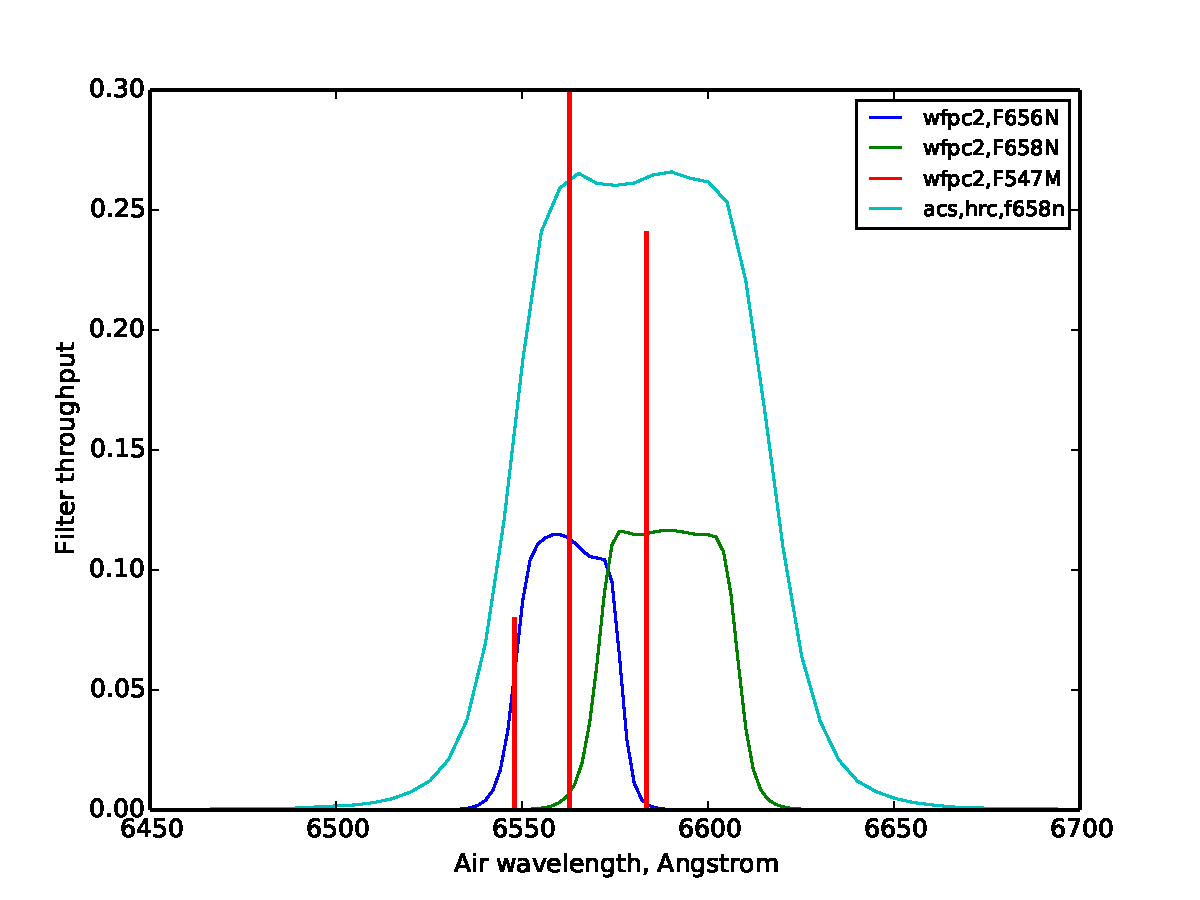
\includegraphics[width=\linewidth, trim=0.7 0.7 0.7 30, clip]{luis-programas/will-filter}
   \caption{Curvas de transmisión de los filtros; F656N y F658N  de la cámara WFPC2 y del filtro F658N de la cámara ACS. Las líneas verticales de color rojo representan en el mismo orden las líneas de emisión de: \nii{} 6548~\A{}, \ha{} 6563~\A{}, \nii{} 6583~\A{}. }
   \label{fig:transmision}
 \end{figure}

Por último, contamos con  las observaciones de unos viejos mosaicos de la cámara WFPC2 como parte del programa GTO-5085. Además de las desventajas de esta cámara mostradas arriba, otra desventaja que tienen estas observaciones es que la cobertura es más restringida, particularmente las observaciones del PC que solo cubren el centro de la nebulosa con un radio menor a medio minuto de arco aproximadamente. Pero estas tienen la ventaja que con la implementación de los filtros f656n y f658n en este programa, se obtuvieron imágenes de \ha{} y \nii{} separadamente, útiles para la verificaión de la calibración del flujo. En este programa se tamaron imágenes del continuo usando el filtro f547m, útil en nuestro caso para hacer la correción del brillo superficial por la contribución del continuo. Finalmente, tenemos un mosaico de unas imágenes de \oiii{}, obtenidas mediante el uso del filtro f502n durante las visitas del \textit{HST}, estas imágenes nos van a permitir ver los objetos de alta ionización en las regiones cercanas del Trapecio donde las estrellas son más débiles comparadas con los arcos vistas con este filtro. Otra utilidad de usar estos datos más antiguos es que nos permite distinguir entre los arcos estacionarios y los ecos de objetos HH por su movimiento propio. A continuación daremos una descripción más detallada del juego de observaciones utilizadas en esta tesis.        

\section{La cámara ACS-WFC, El programa GO-9825 y el filtro F658N }
\label{sec:acs}

La cámara ACS-WFC está basada en un masaico de dos detectores CCD de 2048 \(\times\) 4096 pixel. La óptica del instrumento ofrece una escala espacial de aproximadamente 50~\(\mathrm{mas~pixel^{-1}}\), correspondiendo a un campo de visión  de \(202'' \times 200''\). Junto con esta cámara se cuenta con la presencia del filtro F658N (\ha{} + \nii{}), el cual está destinado al mapeo del material circunestelar de las estrellas con la más alta resolución posible, sobre todo para discriminar fuentes extendidas y evaluar la presencia de emisión circunestelar \citep{Robberto:2013a}.\\

\begin{table}
  \centering
  \small\raggedright
\renewcommand{\arraystretch}{1.5}
  \caption{Observaciones de las cámara ACS y WFPC2}\label{tab:instru}
  \begin{tabular}{l l c c c}
   \hline
   \hline
   Instrumento&      Filtro&      Programa&      Línea de emisión&     Tiempo de exposición (s)\\ \hline
   ACS-WFC&          F658N (Banda ancha)&       GO-9825&       \ha{} + \nii{}&       500\\ 
   ACS-WFC&          F658N (Banda ancha)&        Treasury&   \ha{} + \nii{}&        340\\ 
   WFPC2&            F656N (Banda angosta)&      Treasury&   \ha{}&      400\\
   WFPC2&            f658n&       GTO-5085&      \nii{}&               500\\
   WFPC2&            f656n&       GTO-5085&      \ha{}&                200\\
   WFPC2&            f502n&       GTO-5085&      \oiii{}&              200\\
   WFPC2&            f547m&       GTO-5085&      Continuo&             50\\ 
  \hline
  \end{tabular}
\end{table}
\normalsize

En primer lugar  hemos trabajado con las imágenes de \citet{Bally:2006a}, las cuales son observaciones que han sido obtenidas con la cámara \textit{Wide Field Channel} (WFC) del ACS abordo del \textit{HST}, durante el ciclo 12 del programa GO-9825, donde se obtuvieron 26 imágenes que cubren gran parte de la Nebulosa de Orión, cada imagen fue tomada durante una órbita del \textit{HST}. Las áreas cubierta fueron observadas usando el filtro F658N (\(\ha+\nii\)) y tiempos de exposición de 500 s por punto observado en la nebulosa. Dos posiciones, separadas por \(96''.8\) en el eje-y de los detectores del ACS fueron observados durante cada órbita \citep{Bally:2006a}, correspondiendo a un campo de visión de aproximadamente \(200'' \times 300'' \) para cada imágen resultante \citep{Bally:2006a}. En este sentido las distintas imágenes de la Nebulosa de Orión tomadas durante las 26 órbitas cubrieron un área total de aproximadamente 415 \(\text{arcmin}^{2}\). La figura \ref{fig:fields} muestra la ubicación de cada uno de los 26 campos (visitas) del ACS, donde se han superpuesto en una imagen de \sii{} tomada por el telescopio reflector Mayall ubicado en Kitt Peak cerca de Tucson, para mayor información hechar un vistaso al artículo de \citet{Bally:2001a}. Cada rectángulo representa un campo de cada visita del \textit{HST}.\\

\begin{figure}
  \centering
  \includegraphics[width=.8\linewidth, trim=0.7 0.7 0.7 30, clip]{figuras-tesis/fields-acs-sii.png}
  \caption{Posiciones de los 26 campos del ACS observadas con el \textit{HST} durante el ciclo 12 del programa GO-9825, superpuestas en una imagen de \(\sii\) obtenida con un mosaico de detectores CCD del telescopio reflector Mayall situado en Kitt Peak, Arizona. Los rectágulos representan las imágenes CCD del ACS con un tamaño de \(2046 \times 4096\) pixel cada uno. Esta imagen es tomada de \citet{Bally:2006a}.}
  \label{fig:fields}
\end{figure}

La importancia de utilizar las imágenes de Bally radica en que la señal a ruido es muy buena, debido a que tienen tiempos más largos de exposición, con esto  lograron que el detector CCD recojiera el mayor número de fotones posibles por pixel, implicando que la señal sea muy alta en comparación al ruido. Para nuestro trabajo vamos a utilizar estas imágenes para trazar la forma de los arcos de proa radiativos de las estrellas LL~Ori, puesto que en estas imágenes se logran ver de manera clara los límites de la cáscara chocada y también las utilizaremos para determinar el brillo superficial de \ha{}.\\

Por otro lado, como ya se dijo arriba esta cámara (ACS) contiene el filtro F658N, el cual es un filtro de banda ancha (\(50 \text{Å}\)), que permite obtener imágenes de \ha{} + \nii{}, donde principalmente domina las líneas de \ha{} y en menor grado las líneas de \nii{}. Sin embargo, la desventaja de utilizar estas observaciones es que no tiene una cobertura completa de la Nebulosa de Orión\footnote{Los objetos, LL7 y 4285-458 quedan por fuera de los campos de Bally.} y además estas observaciones están contaminadas por líneas de \nii{}. Por último es importante señalar que de los 26 campos del ACS-F658N que mapean la región, nuestros objetos se encuentran distribuidos en los campos: 01, 02, 06, 07, 08, 09, 14, 16, 17 y 24. En la figura \ref{fig:field-01} se muestra como es la apariencia de uno de estos campos (visita) de la cámara ACS.\\

\begin{figure}
  \centering
  \includegraphics[width=.95\linewidth, trim=60 90 60 60, clip]{figuras-tesis/field-01-acs.pdf}
  \caption{Campo 01 del WFC-ACS; que corresponde a una imagen de \ha{}+\nii{} observadas con el \textit{HST} durante el ciclo 12 del programa GO-9825, usando el filtro de banda ancha F658N, en ella se puede apreciar el Trapecio y algunos choques de proa en sus cercanías.}
  \label{fig:field-01}
\end{figure}

\section{Programa Treasury del Telescopio Espacial Hubble}
\label{sec:wfpc2}

El Programa Treasury del \textit{HST} descrito en el artículo de \citet{Robberto:2013a}, fue destinado para el estudio de las componentes estelares de la ONC en las longitudes de onda del visible. El programa se basa en un total de 104 órbitas (ciclo 13), cubriendo las regiones más brillantes de la Gran Nebulosa de Orión en el rango del espectro electromagnético que caen en el óptico, usando filtros de banda ancha para obtener la fotometría más precisa del mayor número posible de objetos de baja masa presecuencia principal. Las cámaras a bordo del \textit{HST} usadas para este fin son; la ACS-WFC, la  cámara  WFPC2 y la Near-Infrared Camera and Multi-Object Spectrograph (NICMOS), las imágnes de esta última cámara no son consideradas para este estudio. \\    

\paragraph{La cámara ACS-WFC y el filtro F658N.}
Con la cámara ACS como parte del Programa Treasury se tomaron imágenes en el óptico (estrictamente hablando de \ha{}) de la Nebulosa de Orión cubriendo un área total de 627~\(\mathrm{arcmin^2}\) (correspondiendo a 904~Mpix aproximadamente) como resultado de las 104 visitas del \textit{HST}, usando el filtro F658N y a diferencia de las observaciones de Bally un tiempo de exposición de 340 s. En la figura~\ref{fig:field-acs-the} se logran ver las posiciones de los campos de la camara ACS del Programa Treasury superpuestos en una imagen de la Nebulosa de Orión. \\

\paragraph{La cámara WFPC2 y el filtro F656N-\ha{}.}
La cámara WFPC2 actualmente remplazada por la Wide Field Camera 3 usó 4 CCDs de $800\times800$ pixel a bordo del \textit{HST}. Tres de esos detectores comprenden la \textit{Wide Field Camera} (WFC) y tomaron imágenes de \(150''\times150''\) con una resolución espacial de 100~\(\mathrm{mas~pixel^{-1}}\) el campo de visión de estas imágenes tienen forma de ``L''. El cuarto detector conocido como la  Cámara Planetaria (PC) tomó imágenenes más pequeñas esto es de \(34''\times34''\) correspondiendo a una escala espacial de 46~\(\mathrm{mas~pixel^{-1}}\) y su campo de visión son campos cuadrados \citep{McMaster:2008}. Un compendio de imágenes de Robberto tomadas con la WFPC2, han de brindar otra oportunidad de estudiar los arcos LL de la Nebulosa de Orión. Puesto que la ya mencionada WFPC2, ha tomado un conjunto de imágenes que cubren en su mayoría a la Nebulosa de Orión a diferencia de las imágenes de Bally que no tienen una cubertura total de la misma. Se han usado 104 órbitas del \textit{HST} para dicho fin, como parte del Programa Treasury \citep{Robberto:2013a}. En la figura \ref{fig:fields-robberto} se pueden apreciar los campos (visitas) del WFPC2, que entre otras cosas cubren un área total de 570.5 \(\text{arcmin}^{2}\). El tiempo de exposición se puede ver en la tabla~\ref{tab:instru}. \\

\begin{figure}
\centering
  \includegraphics[width=.95\linewidth]{./figuras-tesis/acs-theasury}
\caption{\textit{Izquierda}. Campos de la cámara ACS superpuertos en una imagen de JHK de la Nebulosa de Orión de 2MASS. \textit{Derecha}. Representación de los campos del ACS obtenidas a partir de 104 vistitas del \textit{HST}, como parte del \textit{Programa Treasury}. Mapean una área consirable de la Nebulosa de Orión. Las partes partes mas oscuras son las regiones de solapamiento entre las distintas visitas. También se puede ver el número de identificación de cada campo, para ser referenciado. Imagen tomada de \citet{Robberto:2013a}. }\label{fig:field-acs-the}
\end{figure}

\begin{figure}
  \centering
  \includegraphics[width=.95\linewidth]{figuras-tesis/fields-robberto.jpg}
  \caption{Igual que la figura~\ref{fig:field-acs-the} para los campos de WFPC2.}
  \label{fig:fields-robberto}
\end{figure}

Uno de los filtros usados en este ambicioso programa es el filtro F656N. Este es un filtro de banda angosta de \ha{}, que sólo permite el acceso de estas líneas (\ha{}~\(\lambda = 6563~\text{\AA{}}\)), dejando que sólo pase una mínima cantidad de la radiación de \nii{} (\(\lambda = 6583~\text{\AA{}}\)), que en este estudio consideraremos despresiable. Entonces para este trabajo usamos las observaciones de \citet{Robberto:2013a} (WFPC2) debido a que estas imágenes son sólo de \ha{}. En este orden de ideas, la idea de usar las imágenes de la cámara WFPC2-F656N va a permitir que sea posible separar las emisiones de \ha{} de \nii{} en las imágenes de Bally, subsecuentemente  podremos  utilizar estas imágenes de ACS corregida por \nii{} para determinar parámetros astrofísicos tales como el flujo de momento de los arcos de proa y esto es  porque las observaciones de Bally tienen mejor señal a ruido como se dijo arriba.

\section{Otras observaciones de la cámara WFPC2:  viejos mosaicos}
\label{sec:mosaic}

Para este estudio también se cuenta con unas observaciones, un poco más viejas que mapean una región particular de la Nebulosa de Orión (el centro de la nebulosa). Estas observaciones son el resultado de dos pragramas del \textit{HST}, el primero de estos es el programa GTO-5085 (Guaranteed Time Observer  por su nombre en inglés) cuyo principales investigadores fueron  \citet{Odell:1996} y el segundo corresponde al programa GO-5469 (General Observer por su nombre en inglés) con Jhon Bally como principal investigador. Las imágenes proporcionadas por el programa de Bally fueron usadas principalmente para el estudio de proplyds con una  alta resolución espacial, usando la cámara WFPC2 abordo del \textit{HST}. En estas imágenes el tamaño de lo pixeles es de \(0.0996''\) algo muy característico de las cámaras WF \citep{Holtzman:1995}. Los campos seleccionados para la formación de las imágenes se determinaron de tal manera que tengan una cobertura continua de un área en la parte central de la Nebulosa de Orión, en este sentido se tiene una superposición de los campos, representados através de unos  masaicos de la cámara WFPC2. Se hablan de varios mosaicos puesto que se utilizaron múltiples filtros del programa GTO-5085 para registrar diferentes líneas de emisión. Los extremos de la región mapeada fueron elegidos con el propósito de incluir objetos de particular interés, tales como objetos Herbig-Haro en el norte y los choques de proa en el suroeste \citep{Odell:1996}.\\

 Los filtro usados fueron seleccionados de tal manera que se capturaran las líneas de emisión más fuertes, es decir aquellas que representaran un rango razonable de condiciones de ionización. Por tanto se cuenta con un masaico en el que se usó el filtro f658n, es decir en este mosaico domina sólo la presencia de la línea de emisión \nii{} (6584~\A{}). También se cuenta con un mosaico, en el que sólo dominan las líneas de emisión de \ha{} (6563~\A{}), puesto que para capturar las imágenes se usó el filtro f656n. En esta lista se incluye un masaico cuyas imágenes son el resultado del uso del filtro f502n, donde se han registrado las líneas de emisión de \oiii{} (5007~\A{}), que provienen de regiones con la más alta ionización en la nebulosa. Por último existe un mosaico formado por los campos obtenidos a partir del filtro f547m \citep{Burrows:1995}, este es un filtro suficientemente ancho (en comparación a los demás filtros), ubicado en una región del espectro electromagnético, donde no hay líneas fuertes de emisión, por tanto este mosaico son unas imágenes del continuo. Los tiempos de exposición para cada filtro son: f656n;  200~s, f658n; 500~s, f502n; 200~s, f547m; 50~s para el programa GO-5085. 



% \bibliography{luis-ref}

% \end{document}

\chapter{Metodología observacional}
%\documentclass{article}
%\usepackage[utf8]{inputenc}
%\usepackage{amsmath}
%\usepackage{natbib}
%\usepackage{graphicx}
%\usepackage{astrojournals} % Necesario para nombres de revistas en luis-ref.bib
%\usepackage[spanish, es-minimal]{babel}
%\usepackage{longtable}
%\usepackage{geometry}
%\usepackage{multirow, array}
%\newlength\figwidth
%\setlength\figwidth{0.48\textwidth}
%\bibliographystyle{apj}


%\title{Catalog of stationary bowshock arcs in the Orion Nebula}

%\author{
  %Alumno: Luis Angel Gutiérrez Soto\\
  %Tutor: Dr. William Henney
%}
%\begin{document}
%\maketitle

%\section{Metodología}
\label{chap:methodology}
Como uno de los objetivos de esta tesis es realizar un catálogo completo de los choques de proa en la Nebulosa de Orión, el primer paso llevado cabo en esta tarea fue la identificación y la busqueda, en las imágenes del \textit{HST} descritas en el capítulo anterior, de los arcos de emisión ya conocidos. Entonces un grupo de 6 proplyds llamados: 168-326 (LV1), 167-317 (LV2), 166-316 (LV2b), 163-317 (LV3), 161-324 (LV4) y 158-323 (LV5) detectados y mostrados por  \citet{Laques:1979} fueron buscados e identificados como parte de este trabajo en las observaciones ya mencionadas. Es importante subrayar que Laques \& Vidal no observaron los arcos, estos fueron descubiertos hasta la década de los 90. Muchos de estos arcos de emisión fueron reportados en varios artículos de Bally. Algunos aparecen en el artículo de \citet{Bally:2000a} y son los siguientes: w000-400, w005-514, w012-407, w014-414, w030-524, w044-527, w056-519, w069-601, w073-227 y w266-558. Los objetos designados con los nombres desde LL1 a LL7 fueron catálogados por primera vez por \citet{Bally:2001a}. Varios objetos aparecen en una lista presentada por \citet{Bally:2006a}. Estos son los que se llaman LL4, LL5, etc que son los mismos mostrados por \citet{Bally:2001a}, pero otros objetos también son presentados en este artículo tales como; 4468-605, 116-3101, 203-3039, 261-3018, 305-811, 308-3036 y 344-3020. Dos choques de proa producidos por la interacción de los flujos de dos proplyds son mostrados en \citet{Reipurth:2007}, estos objetos de interacción interproplyd son: 066-652, donde su choque se genera por la colisión con el viento del proplyd 066-652N y 162-456, el cual interacciona con el proplyd 162-456NE. En un catálogo de \citet{Ricci:2008} son mostrados muchos proplyds y supuestos proplyds. En esta lista aparecen: 066-3251, 121-434, 124-131 y 178-258. En nuestra busqueda encontramos cerca de 20 objetos nuevos (no reportados antes en la literatura), que se podrán ver más adelante cuando presentamos el catálogo completo. \\         

Después de haber detectado todos los choques de proa en las ya mencionadas observaciones, se hizo la caracterización de estos objetos, es decir, se trazaron la forma de los arcos de los choques de proa estacionarios, usando las herramientas del programa ds9 SAO image, para medir los radios característicos (\(R_{c}\) y \( R_{0}\)). También se estimaron las distancias (\(D\)) de las fuentes a \thC{}, se determinaron las anchuras (\(h\)) de las cáscaras y se  midieron  los valores de la emisión en las imágenes de las cámaras ACS y WFPC2 y se hicieron las pertinentes calibraciones del flujo.

\section{Formas de los arcos}
\label{sec:arcos}

Como primer paso para caracterizar los arcos de los objetos LL en las afueras de las nebulosa y de los proplyds interiores, se trazaron las formas de los mismos. Para ello establecimos las posiciones donde pensamos que se encuentran los arcos de proa con el propósito de delimitar la cáscara formada por los dos choques (internos y externos) como se puede ver en la figura \ref{fig:arco-LL1}. Esto se hizo usando el contraste de brillo entre los choques de proa o las cáscaras y el fondo, debido a que los choques son fuertemente radiativos generando que los arcos sean muy brillantes y esto es lo que vemos en las imágenes. Estos argumentos nos dan las pautas para distinguir la emisión en las dos regiones (en la cáscara chocada y en el fondo) y así poder trazar los arcos. Este procedimiento es un tanto subjetivo porque es un estimador a simple vista de donde se encuentran los choques. No obstante, para reducir los aspectos subjetivos se implementaron algunas herramientas del ds9 SAO image, utilizando los contornos para trazar los bordes de la cáscara chocada. Además se usaron las imágenes en los diferentes filtros donde se ven mejor los choques para trazar los arcos. Por ejemplo, en las regiones internas de la nebulosa se usaron imágenes de \oiii{}~\(\lambda5007\) para trazar algunos arcos debido a la alta ionización del gas en esta zona. Para las regiones externas de la nebulosa, donde las líneas de baja ionización de \nii{}~\(\lambda6584\) son importantes, se utilizaron imágenes del filtro F658N para trazar la forma de algunos arcos LL. También nos dimos cuenta que algunos arcos se ven muy bien en el continuo así que se usaron imágenes del filtro f647m para este fin, aunque para la mayoría de los casos se usaron las imágenes de \ha{} + \nii{}.\\

Por otro lado, estas estructuras deben cumplir los siguientes criterios para poder ser catálogados como arcos. Primero, en el caso de los proplyds interiores los ejes de los choques deben coincidir con el eje del proplyd y estos deben estar orientados hacia \thC, a excepción de los arcos formados por la interacción de dos proplyds donde se toma como eje de referencia uno de los proplyds y donde el choque está orientado hacia el otro proplyd. Ademas en el caso de los proplyds los arcos tienden a tener formas  semi-circulares entorno a los proplyds. Segundo, en el caso de los objetos LL situados en las regiones mas alejadas de la nebulosa sus arcos tienen forma más hiperbólica y están justo en frente de la estrella presecuencia principal, orientados hacia el núcleo de la nebulosa.  Para separar los arcos de los objetos HH se usaron imágenes de diferentes filtros, puesto que como se puede ver en la figura \ref{fig:LL1} del capítulo \ref{chap:introduction} el objeto HH asociado a la estrella T-Tauri de LL1 muestra unos nudos muy brillantes en los diferentes filtros que parecen no seguir la forma del arco de proa. 


\begin{figure}
  \centering
   \includegraphics[width=.6\linewidth]{figuras-tesis/forma-LL1.jpg}
  \caption{Formas de los arcos para LL1, donde los bordes de los choques están delimitados por los puntos: ``x'', para trazar el borde externo y ``+'', para trazar el borde interno. Para determinar la posición de la estrella se usaron pequeños círculos o puntos esto se hizo usando las herramientas del programa ds9 sao image. Esta imagen es tomada del campo 01 de \citet{Bally:2006a} (ACS-F658N) en el sur-oeste de la Nebulosa de Orión, por tanto es una imagen de \ha{}+\nii{}. }
  \label{fig:arco-LL1}
\end{figure}

\section{Estimación de los parámetros. \(D\), \(R_{0}\) , \(R_{c}\) y \(h_{0}\) }
\label{sec:parametros}

El propósito de trazar los arcos hiperbólicos radica en que con esta información (coordenadas) es posible estimar varios parámetros observacionales, que nos permiten extraer información acerca de los choques. En este orden de ideas, una vez que ya teníamos las posiciones tanto de las componentes de los choques como de la estrella misma se pudo establecer la distancia proyectada \(D\), desde la fuente a \thC{}; esta medida nos resultará muy útil como veremos más adelante. De la misma manera se midió \(R_{0}\), este radio lo vamos a definir como la distancia a lo largo del eje de simetría, de la fuente\footnote{La fuente podría ser una estrella T-Taury o un proplyd. Objetos de los cuales se origina el viento interno.} \citep{Robberto:2005}  al borde externo o interno de la cáscara chocada, dependiendo de cual sea el caso. El eje de simetría es la línea proyectada en la dirección en que están orientados los arcos; en la figura \ref{fig:radios} y \ref{fig:anchura} está representada por la línea amarilla. No obstante, hay que aclarar que tenemos dos radios debido a la presencia de un borde externo e interno, como ya se ha visto. \\ 

\begin{figure}[htp]
\centering
\begin{tabular}{l l}
(\textit{a}) & (\textit{b})  \\
  \includegraphics[width=0.45\linewidth, trim=40 0.98 40 50, clip]{./figuras-tesis/177-341-Bally-01-images-sin.jpg}&
 \includegraphics[width=0.45\linewidth, trim=40 0.98 40 50, clip]{./figuras-tesis/177-341-Bally-01-images.jpg}\\
\end{tabular}
\caption{(\textit{a}) Proplyd 177-341 ubicado en el sureste de la Nebulosa de Orión. (\textit{b}) Mismo proplyd con una representación de los radios característicos: \(R_{0}(\Out{})\); que es el radio del choque externo, medido a lo largo del eje que va desde el proplyd a \(\theta^1\ \text{Ori}\ \text{C}\), este eje está representado por la línea amarilla. \(R_{c}(\Out{})\) y \(R_{c}(\In{})\); llamados radios de curvaturas, son los radios de los círculos ajustados a partir de los puntos (coordenadas) utilizadas para delimitar los bordes externo e interno de la cáscara chocada. }\label{fig:radios}
\end{figure}

Por otro la lado, se han determinado los radios de curvaturas \(R_{c}\), que son los radios de los círculos que se han ajustado, utilizando los puntos con los cuales hemos trazado la forma de los choques (ver figura \ref{fig:radios}). Se han medido los radios de curvatura para el borde interno y el borde externo de la cáscara chocada y los hemos llamado \(R_{c}(\Out{})\) y \(R_{c}(\In{})\), respectivamente. Es de notar que la posición de la estrella no corresponde con el centro de los dos círculos que hemos fijado, en otras palabras las posiciones de los centros de los círculos dependen de la forma de los arcos que hemos trazado, es así que estos radios (obtenidos a partir de los cículos ajustados) van a ser un indicador de que tan simétricos son los choques, puesto que como podemos ver en la figura \ref{fig:anchura}, el centro de los círculos no coincide con el eje, entonces estaríamos frente a un caso de un choque que no es rigurosamente simétrico.\\

Siguiendo con la metodología llevada a cabo, otro parámetro que hemos podido estimar ha sido la anchura \(h_{0}\), que como veremos va a ser muy importante para determinar características físicas de los choques, \(h_{0}\) la definiremos como el ancho de la cáscara chocada a lo largo del eje de simetría. Por tanto para determinar éste parámetro hemos hecho lo siguiente: a la distancia que se ha estimado desde el borde externo a la estrella o Proplyd (\(R_{0}(\Out{})\)) le hemos restado el radio del choque interno (\(R_{0}(\In{})\)) (ver figura \ref{fig:anchura}), en esta medida tendremos que la anchura está dada por \(h_{0} = R_{0}(\text{out}) - R_{0}(\text{in})\), que es desde luego también estimado a lo largo del eje del objeto.

\begin{figure}[htp]
\centering
\begin{tabular}{l l}
(\textit{a}) & (\textit{b})  \\
  \includegraphics[width=0.45\linewidth, trim=40 0.98 30 10, clip]{./figuras-tesis/042-628-Bally_16-images.jpg}&
 \includegraphics[width=0.45\linewidth, trim=40 0.98 30 10, clip]{./figuras-tesis/042-628-Bally_16-images-radii.jpg}\\
\end{tabular}
\caption{(\textit{a}) Proplyd 042-628 y su respectivo choque de proa. (\textit{b}) En esta imagen se puede apreciar el mismo proplyd 042-628  con una representación de la anchura \(h_{0}\) y del radio del choque interno \(R_{0}\) a lo largo del eje proplyd-estrella ionizadora. El eje está representado por la línea amarilla.}\label{fig:anchura}
\end{figure}


\section{Estimación y calibración final del flujo-líneas de emisión en las imágenes del ACS y WFPC2}
\label{sec:clibration-final}

\subsection{Determinación de los valores  de la emisión en las imágenes del ACS y WFPC2 }
\label{sec:brillo-superficial}
Otras de las cosas que hemos realizado con nuestros objetos de estudios, ha sido determinar el brillo superficial de cada uno de ellos. Una vez que hemos trazado la forma de los arcos hiperbólicos, se han extraído de los campos de Bally (que cubren en su mayoría a la Nebulosa de Orión), pequeñas imágenes FITS que sólo abarcan las regiones donde se encuentran los objetos LL y los proplyds, con el propósito de facilitar las mediciones de los valores del flujo de las imágenes. Esto mismo se hizo con los campos de Robberto. Así que usando estas pequeñas imágenes hemos medido los valores del flujo de las imágenes\footnote{En el caso de de las campos de Bally los valores de la emisión de las imágenes tienen unidades de \(\mathrm{electrones~s^{-1}~pixel^{-1}}\) y en caso de las imágenes de Robberto tienen unidades de \(\text{counts}~\text{s}^{-1}~\text{pixel}^{-1}\).} en un determinado número de puntos o pixeles a lo largo de diferentes ángulos \(\theta\) en la región chocada y en el fondo, donde se ha supuesto que \(\theta = 0\) corresponde al eje proyectado en el plano del cielo que sigue la dirección en que llegan los fotones ionizantes provenientes de la estrella masiva y todos los demás ángulos \(\theta\) se forman a partir de dicho eje, en sentido contrario a las manecillas del reloj. Para ser más didácticos miremos un caso particular de los resultados de tales mediciones. La figura \ref{fig:brillo-theta} nos muestra los valores en función de \(\theta\) para w005-514, es de notar que esta gráfica permite ver los valores en el fondo, en la zona chocada y más rigurosamente en el centro de la cáscara. Estas mediciones se hicieron tomando la imágenes de la cámara ACS-F658N y de la misma manera se procedió con las imágenes del WFPC2-F656N \citep{Robberto:2013a}. \\

\begin{figure}[htp]
\centering
\begin{tabular}{l l}
(\textit{a}) & (\textit{b})  \\
  \includegraphics[width=0.5\linewidth, trim=60 10 70 50, clip]{./j8oc01010_wcs/w005-514-Bally_01-arcbright-th.jpg}
& \includegraphics[width=0.5\linewidth, trim=60 10 70 50, clip]{./j8oc01010_wcs/w005-514-Robberto_WFPC2_27_f656n-arcbright-th.jpg}\\
\end{tabular}
\caption{Valores de la emisión o brillo superficial para el proplyd w005-514 en unidades de [\(\text{electrones}~\text{s}^{-1}~\text{pixel}^{-1}\)], en función de los ángulos \(\theta\). Los puntos representan los pixeles individuales y los colores representan la distancia con respecto a los arcos (\(z = (R - R_{\text{in}})/(R_{\text{out}} - R_{\text{in}})\)). Las líneas indican las medianas de los valores en el centro de la cáscara y en el fondo y las bandas de colores representan el rango entre los cuartiles. Para separar los pixeles de la cáscara del fondo se usaron las coordenadas de los bordes internos y externos medidos a partir de la diferencia de contraste en la emisión en las imágenes del \textit{HST}.}\label{fig:brillo-theta}
\end{figure}


Por otro lado también se determinaron los valores del brillo superficial en función de la posición con respecto a los arcos, dicha posición se ha escrito de la siguiente forma; \(z = (R - R_{\text{in}})/(R_{\text{out}} - R_{\text{in}})\), que serían los radios relativos a la cáscara, donde \(R\) es la separación radial, \(R_{\text{out}}\) es el radio  desde la estrella al borde externo y \(R_{\text{in}}\) es el radio desde  la estrella al borde interno, es así que la figura \ref{fig:brillo-z} ilustra cuales son los valores para las diferentes radios relativos \(z\). Hay que resaltar que este tipo de gráficas las obtuvimos para cada uno de los choques estacionarios.\\
\begin{figure}[htp]
\centering
\begin{tabular}{l l}
(\textit{a}) & (\textit{b})  \\
  \includegraphics[width=0.5\linewidth, trim=60 10 70 50, clip]{./j8oc01010_wcs/w005-514-Bally_01-arcbright-z.jpg}
& \includegraphics[width=0.5\linewidth, trim=60 10 70 50, clip]{./j8oc01010_wcs/w005-514-Robberto_WFPC2_27_f656n-arcbright-z.jpg}\\
\end{tabular}
\caption{Valores del brillo superficial para el proplyd w005-514 en función de la posición  \(z = (R - R_{\text{in}})/(R_{\text{out}} - R_{\text{in}})\). La líneas indican los valores del brillo para diferentes intervalos de angulos \(\theta\).  Para (\textit{a}) WCS F658N (\textit{b}) WFPC2 F656N.}\label{fig:brillo-z}
\end{figure}

Dado que se tenían los valores de la emisión de los pixeles para las diferentes zonas de los choques hiperbólicos como se mencionó arriba, entonces como siguiente paso se determinaron los valores promedios en la cáscara chocada, en el fondo y en el centro de la cáscara. Para ello se implementaron los conceptos de  estadística robusta, que consistió en determinar el ``trimean'' en las diferentes zonas de nuestros objetos (en la cáscara chocada, en el fondo y en el centro de la cáscara). El trimean es definido como el promedio ponderado de la mediana y los dos cuartiles\footnote{En estadística descriptiva los cuartiles son los tres valores que dividen al conjunto de datos ordenados en cuatro partes porcentuales iguales.}. Entonces de acuerdo a esta definición primero fue necesario encontrar los tres cuartiles de los datos; \(q_{1}\), \(q_{2}\) y \(q_{3}\). Luego con la  ecuación \(\text{TM} = 0.25(q_{1} + 2q_{2} + q_{3})\) se calcularon los trimean o los valores promedios del brillo, para el conjunto de pixeles situados en el intervalo angular \(\theta < 45^{\circ}\) en las regiones ya mencionadas de los objetos LL. Por otro lado se estimó el rango intercuartil el cual es la diferencia entre el tercero y primer cuartil (\(q_{3} - q_{1}\)), obteniendo una medida de la dispersión de nuestros datos. De la misma manera, es decir usando estadística robusta, se determinaron el promedio de los valores del brillo para distintos ángulos \(\theta\) (ver figura~\ref{fig:brillo-theta}), y usando el rango intercuartil estimado para cada ángulo \(\theta\) se determinó la anchura de la distribución, que rescalada nos permitió  estimar la desviación estandar y las incertidumbres para una distribución Gaussiana de nuestro juego de datos. \\
 
Hay que tener en cuenta que los valores determinados para las cáscara incluyen los del fondo. Para tener unos valores coherentes del mismo, es decir sólo de la cáscara, le hemos restado los valores del fondo. Es importante mencionar que de la misma manera hemos medido los valores de la emisión de las  imágenes de los viejos  mosaicos de WFPC2, es decir aquellas  observaciones obtenidas con el uso de los filtros F656N (\(\mathrm{\ha~6563~\A{}}\)), F658N (\(\mathrm{\nii~6583~\A{}}\)), f502n (\(\oiii{}~5007~\A{}\)) y del filtro para el continuo f547m.\\

\subsection{Estimación de las constantes de calibración}

\label{sec:const}
En esta parte del trabajo hemos escrito los valores de las emisiones medidos en las observaciones de las respectivas cámaras, en unidades físicas, esto es en [\(\mathrm{erg\ s^{-1}\ cm^{-2}\ sr^{-1}}\)]. Como ya se dijo, los valores medidos en las imágenes tomadas por la cámara ACS con el filtro F658N tienen unidades de [\(\mathrm{electrones\ s^{-1}}~\text{pixel}^{-1}\)] y las unidades de los valores en las imágenes de WFPC2 con el filtro F656N tienen unidades de [\(\text{counts}\ \text{s}^{-1}~\text{pixel}^{-1}\)], entonces se realizó la respectiva conversión de unidades con el propósito de tener el brillo superficial obtenido a partir de las imágenes de las cámaras ACS y WFPC2 en las mismas unidades físicas.\\

\subsubsection{Estimación de las constantes de calibración de las imágenes de Bally (ACS-F658N) y Robberto (WFPC-F656N)}
\label{sec:acs}

Las estimaciones de las constantes de calibración del flujo en las imágenes del \textit{HST}, se pueden hacer de dos maneras. La primera forma de hacerlo consiste en usar las características de los detectores y los filtros medidos en el laboratorio antes del lanzamiento. Dicho de otra forma, este método se basa en utilizar la información clave que aparece en los encabezados de las imágenes del \textit{HST}. Esta información es mantenida en los archivos de imágenes después del lanzamiento y puede ser recuperada posteriormente por usuarios externos a través de un visor de imágenes tal como ds9. La segunda manera de hacerlo consiste en intentar hacer una calibración empírica cuando el instrumento ya está en órbita, mediante la comparación con espectros fotométricos terrestres. El problema de este método es que se requieren demasiados recursos del \textit{HST}, esto quiere decir que toma demasiado tiempo que podría utilizarse en las observaciones directas. Por otro lado no es muy satisfactorio hacerlo de esta manera debido a las limitaciones de las fuentes de referencia astrónomicas disponibles \citep{McMaster:2008}. Así que en este trabajo se ha inplementado el primer método descrito arriba para hacer las calibraciones de las imágenes de Bally (cámara ACS-F658N) y de Robberto (cámara WFPC2-F656N).\\     

 Para la estimación de los coeficientes de calibración obtuvimos la información clave para la fotometría, del encabezado de las imágenes FITS a través del programa de visualización y análisis ds9. Una de estas informaciones es el PHOTFLAM el cual está definido como la densidad de flujo promedio \(F_{\lambda}\) en unidades de [\(\mathrm{erg~cm^{-2}~\A{}^{-1}~electrones^{-1}}\)] que producen 1 cuenta\footnote{Cuentas puede referirse a DN o electrones dependiendo del instrumento. En este contexto DN es la sigla en inglés de \textit{número de datos}. El \(\mathrm{e^{-}}\) acumulado en cada píxel se representa mediante un número en "unidades" de un DN } por segundo en las observaciones del \textit{HST}. Primero determinamos la constante de calibración para las imágenes de la cámara ACS y el filtro F658N. Como se mencionó en la sección~\ref{sec:brillo-superficial} las imágenes están en unidades de [\(\mathrm{electrones~s^{-1}~pixel^{-1}}\)], es así que si se multiplican por el PHOTFLAM (a este parámetro también se le llama ``inverse sensitivity'' en el encabezado de las imágenes fits), se obtienen unidades de [\(\mathrm{erg\ s^{-1}~cm^{-2}~\A{}^{-1}~pixel^{-1}}\)]. No obstante al multiplicar por la anchura rectangular del filtro nos libramos del término \A{} y al dividir por el área del pixel, información que también se obtuvo del encabezado, vemos que se pueden escribir los valores de las imágenes en unidades de brillo superficial [\(\mathrm{erg~s^{-1}~cm^{-2}~sr^{-1}}\)]. De acuerdo a este análisis se estimó el valor de la constante de calibración del flujo en las unidades adecuadas, que es presentada en la tabla~\ref{tab:table-constans}. La anchura rectangular es diferente del PHOTBW que aparece en el encabezado y no está incluido en este. Lo calculamos separadamente usando una paquetería de python llamado ``pysynphot'', dando como resultado 74.9405 \(\text{\AA{}}\).\\

En segundo lugar se determinó el coeficiente de calibración  para las imágenes de \citet{Robberto:2013a} (WFPC2-F656N). Esto se hizo usando el mismo procedimiento descrito arriba (calibración del brillo en las imágenes de Bally), para escribir en unidades de brillo superficial los valores de la emisión \(\ha{}~6563~\A{}\) de estas imágenes. Aunque es de notar que para este caso se obtuvo para la anchura del filtro un valor de 28.34207~\A{}. El coeficiente de calibración resultante se puede ver en la tabla~\ref{tab:table-constans}.\\

\subsubsection{Estimación de las  constantes de calibración de las imágenes de los mosaicos de WFPC2}
\label{sec:wpfc2}
Las imágenes de los viejos mosaicos del WFPC2  obtenidas con el filtro f656n (\(\mathrm{\ha~6563~\AA{}}\)) y el filtro f658n (\(\mathrm{\nii~6583~\AA{}}\)) están unidades de [conteos], así que para obtener unidades de brillo superficial, también se estimó el coeficiente de calibración para estas observaciones. Para determinar dichas constantes de calibración se hizo el siguiente análisis. Para obtener unidades de [\(\mathrm{count~s^{-1}}\)] hay que  dividir entre el tiempo de exposición, teniendo en cuenta que las observaciones tomadas con el filtro F656N tiene un tiempo de exposición de 200~s y las del filtro F658N tiene un tiempo de exposición de 500~s. Ahora, si estos valores en unidades de [\(\mathrm{count~s^{-1}}\)], se dividen entre los coeficientes de calibración de \citet{Odell:2009}, los cuales ha llamado \(\mathrm{K1_{filter}}\) y respectivamente tienen por valor: \(\mathrm{K1_{F656N} = 1.62}\) y \(\mathrm{K1_{F658N} = 160}\) con unidades de [\(\mathrm{10^{-10}~counts~cm^{2}~sr~photons^{-1}}\)], se obtienen unidades de [\(\mathrm{photons~s^{-1}~cm^{-2}~sr^{-1}}\)]. Por último, al multiplicar por la energía del fotón (\(\mathrm{E=3.027\times 10^{-12}~erg~para~\ha{}~6563~\AA{}}\) y \(\mathrm{E=3.018 \times10^{-12}~erg}\) para \(\nii{}~6583~\A{}\)) se obtienen cantidades con unidades de [\(\mathrm{erg~s^{-1}}\)  \(\mathrm{cm^{-2}~sr^{-1}}\)] que al final de cuentas es lo que se quiere.  Con este análisis concluimos que al realizar la operación \(\text{E}/(\mathrm{K1_{fiter}}\))  podemos obtener las constantes de calibración deseadas, teniendo en cuenta que hay que dividir previamente los valores de las imágenes entre T (el tiempo de exposición) y donde E es la energía del fotón. En la tabla~\ref{tab:table-constans} se pueden apreciar los valores de los coeficientes para F656N y F658N.


\begin{table}[!hb]
\centering
\small\raggedright
\renewcommand{\arraystretch}{1.7}
\caption{Valores de los coeficientes de calibración.}
  \label{tab:table-constans}
\setlength\tabcolsep{2.3pt}
\begin{tabular}{ |l| |c| |l| }
\hline
Cámara-filtro&                       Coeficiente de calibración&       Unidades\\ \hline 
ACS-F658N (Imágenes de Bally)&       0.00250 &                          \(\mathrm{erg~electrones^{-1}~cm^{-2}~sr^{-1}}\)\\
WFPC2-F656N (Imágenes de Robberto)&  0.16896 &                          \(\mathrm{erg~counts^{-1}~cm^{-2}~sr^{-1}}\)\\
WFPC2-F656N (Mosaico)&               0.01868 &                          \(\mathrm{erg~counts^{-1}~cm^{-2}~sr^{-1}}\)\\
WFPC2-F658N (Mosaico)&               0.01886 &                          \(\mathrm{erg~counts^{-1}~cm^{-2}~sr^{-1}}\)\\ 
\hline
 \end{tabular}
 \end{table}
\normalsize

\subsection{Corrección por extinción}
\label{sec:extintion}

Una vez que teníamos los valores fotómetricos y calibrados en flujo, como siguiente paso se realizó la corrección por extinción. Para ello se ha usado un mapa de extinción de \(\text{H}\beta\) junto al siguiente análisis para calcular el flujo corregido por extinción. Entonces para encontrar una expresión del flujo intrínseco en términos de la corrección \(C_{\text{H}\beta}\) y el flujo observado \(F'\), se ha usado la extinción logarítmica \(C_{\text{H}\beta} = -\log(F'/F) = -\log (\text{exp}(-\tau)) = 0.4343\tau\) (con \(F'/F = \text{exp}(-\tau)\)),  la extinción en magnitud \(A_{\text{H}\beta}=-2.5\log(F'_{\text{H}\beta}/F_{\text{H}\beta})\) para  \(\text{H}\beta\), donde  \(F\) es el flujo intrínsico y \(F'\) es el flujo observado. Y la extinción absoluta  

\begin{equation}
A_{\lambda}=-2.5\log(F'_{\lambda}/F_{\lambda})=2.5C_{\lambda}=1.086\tau
\label{eq:exti}
\end{equation}

Ahora bien, de acuerdo a las anteriores expresiones, la extinción nebular se puede escribir como la extinción logarítmica \(C_{\lambda} = C_{\text{H}\beta}(A_{\lambda}/A_{\text{H}\beta})\), sustituyendo esta última expresión en la Ec. \ref{eq:exti} se obtiene que  \(F_{\lambda} = F'_{\lambda}\times10^{C_{\text{H}\beta}(A_{\lambda}/A_{\text{H}\beta})}\). No obstante si  \(f_{\lambda}= E_{\lambda-\text{H}\beta}/A_{\text{H}\beta}\) como han mencionado \citet{Costero:1970} y dado que \(E_{\lambda-\text{H}\beta}=A_{\lambda}-A_{\text{H}\beta}\), entonces se tendrá que \(f_{\lambda} = (A_{\lambda}/A_{\text{H}\beta})-1\) y esto lleva a concluir que \(C_{\lambda}= C_{\text{H}\beta}(1+f_{\lambda})\). De este modo el flujo corregido por extinción se puede escribe de la siguiente forma

\begin{equation}
  \label{eq:flujo}
  F_{\lambda} = F'_{\lambda}\times10^{C_{\text{H}\beta}(1+f_{\lambda})}
\end{equation}

 Donde se tiene que \(C_{\text{H}\beta}\) es la corrección de enrrojecimiento en \(\mathrm{H\beta}\) y \(f_{\lambda}\) es la función de enrrojecimiento normalizada en \(\mathrm{H\beta}\) con \(f_{\beta}=0.0\) \citep{Peimbert:1977}. Para \(\ha{}~(6563~\A{})\) la función de enrrojecimiento es \(f_{\lambda} = -0.220\) \citep{Blagrave:2007}. Por otro lado \(C_{\text{H}\beta}\) es determinado mediante la comparación del valor teórico esperado para una temperatura y una densidad electrónica con el valor observado de la nebulosa, utilizando el hecho de que el cociente entre dos líneas de recombinación de hidrógeno es casi constante (\citeauthor{Peimbert:1977}). Así que con la Ec. \ref{eq:exti} determinamos el flujo corregido por extinción.

\subsection{Corrección por emisión de \nii{}}
\label{sec:comp}

\begin{figure}[htp]
\centering
\begin{tabular}{l l}
(\textit{a}) & (\textit{b})  \\
  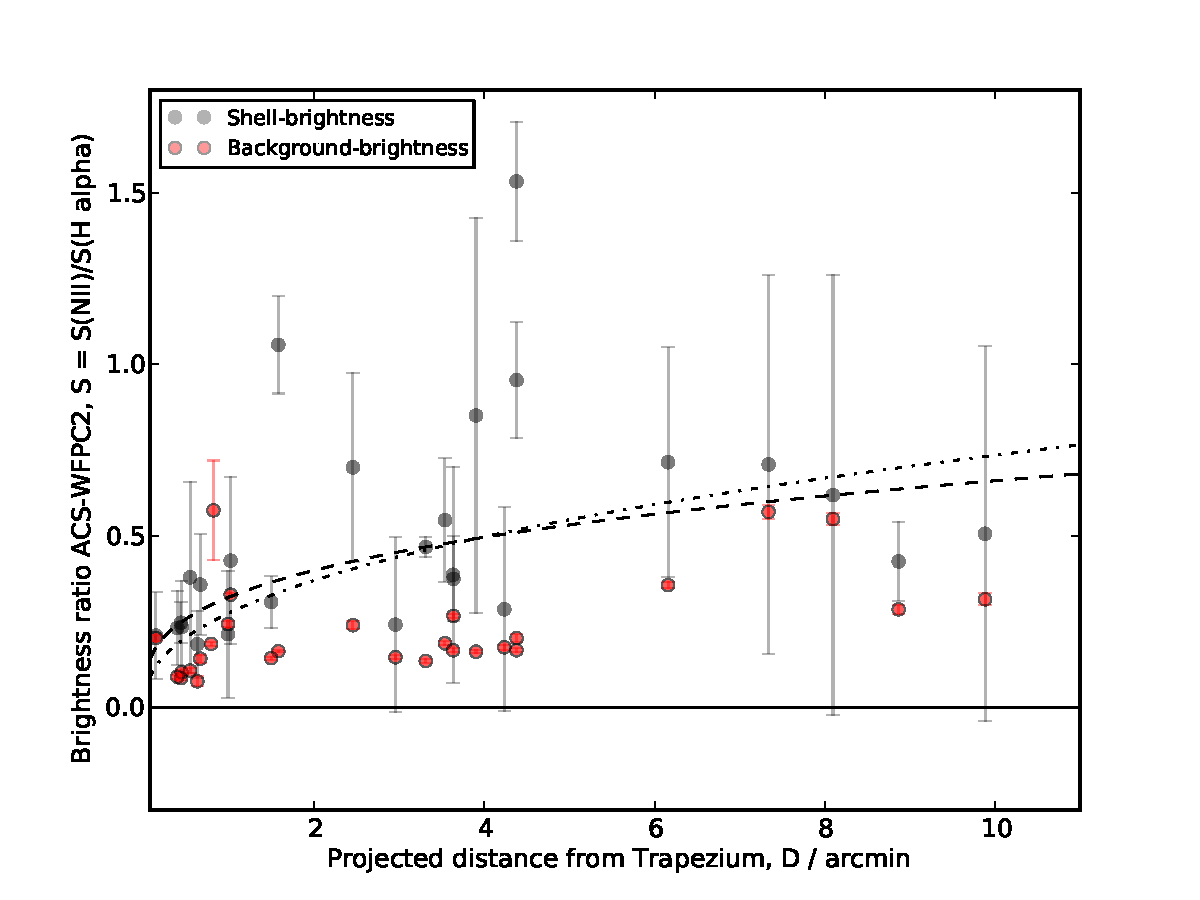
\includegraphics[width=0.48\linewidth, trim=20 9.5 50 20, clip]{./acs_wfpc2-ratio-Nii_ha-vs-D_-mean-error_new}
& 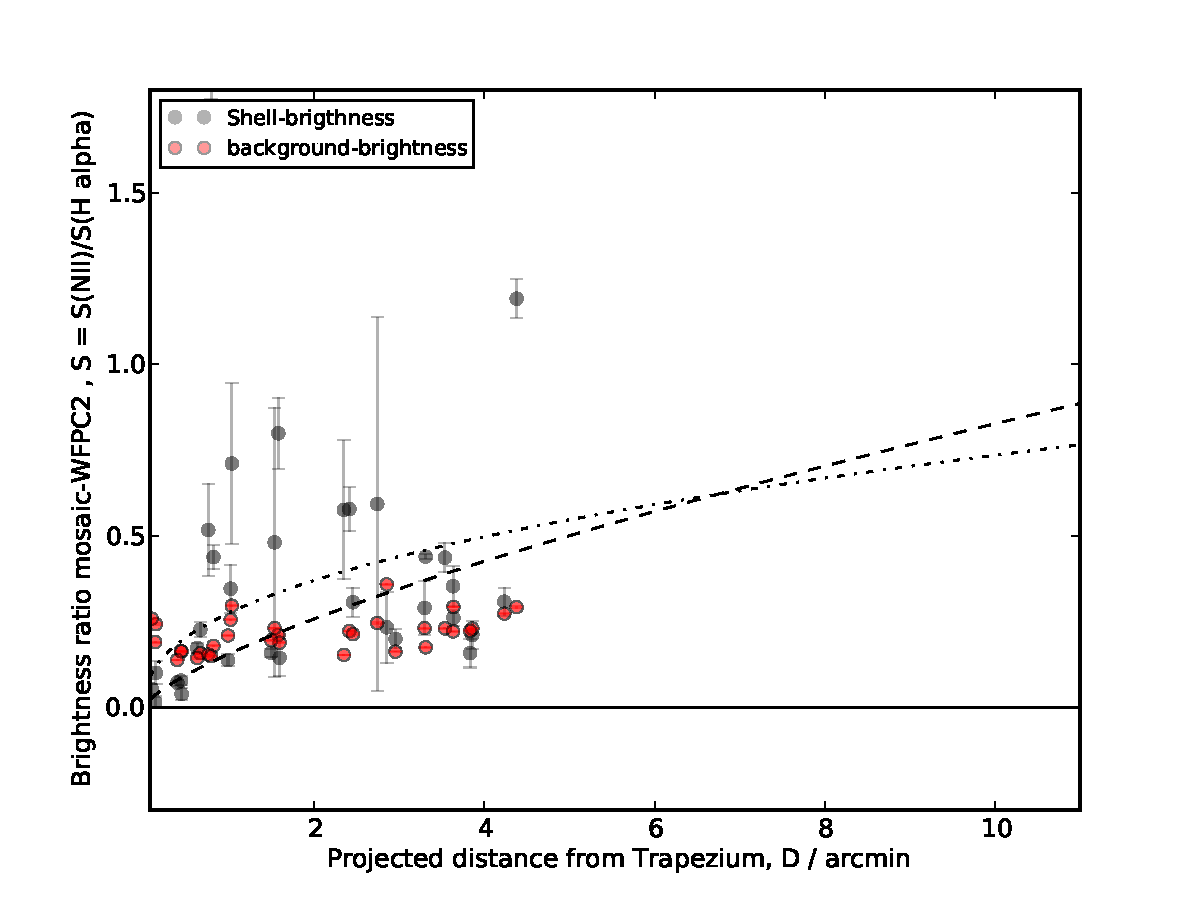
\includegraphics[width=0.48\linewidth, trim=20 9.5 50 20, clip]{./wfpc2-mosaic-ratio-Nii_ha-vs-D_-mean-error_new}\\
\end{tabular}
\caption{Cociente entre el brillo superficial de \nii{} y el brillo superficial de \ha{}, para la cáscara corregida por el fondo (símbolos de color negro) y para el fondo (símbolos de color rojo) en función de la distancia proyectada. (\textit{a}) Usando las observaciones de Robberto, es decir las imágenes de \ha{} de la cámara WFPC2-F656N y las de Bally es decir, las imágenes de \ha{}+\nii{} de la cámara ACS-F658N. La línea discontinua representa un ajuste de un polinomio a los punto graficados la de cáscara chocada cuya relación resultante del ajuste es \(S(\nii{})/S(\ha{})=0.32D^{0.31}\). (\textit{b}) Para el mismo fin se usaron las imágenes de los mosaicos de \ha{} y \nii{} de la cámara WFPC2. La línea discontinua representa lo mismo que en (\textit{a}), pero en este caso son para los datos del mosaico y la relación resultante es \(S(\nii{})/S(\ha{})=0.16D^{0.72}\). La línea de puntos en ambas figuras es un  ajuste  por la combinación de los dos pares de juegos de datos, esto es, las imágenes de Bally y Robberto con las imágenes de los mosaicos del WFPC2, la relación de este ajuste es \(S(\nii{})/S(\ha{})=0.28D^{0.43}\).}\label{fig:ratio-nii-ha}
\end{figure}

La figura \ref{fig:ratio-nii-ha} nos muestra el cociente de brillo superficial de \nii{} entre el brillo de \ha{} \(S(\nii{})/S(\ha{})\), para la cáscara corregido por el fondo, usando las imágenes de la cámara WFPC2-F656N es decir, el brillo de \ha{} extraído previamente de estas imágenes (observaciones de Robberto) y de la cámara ACS-F658N, es decir imágenes de \ha{}+\nii{} (observaciones de Bally), este cociente se estimó usando la relación \(S(\nii{})/S(\ha{}) = (S(\ha{}+\nii{})/S(\ha{}))-1\). Simultáneamente se encontró la fracción \(S(\nii{})/S(\ha{})\) usando las observaciones de dos mosaicos de la cámara WFPC2\footnote{Usando los filtros f656n y f658n.}, puesto que uno de estos mosaicos son imágenes de sólo \ha{} y el otro son imágenes de sólo \nii{}, esto nos permitió  calcular el cociente de brillo más directamente, debido a que en principio estos datos son más confiables, no obstante el problema de estas observaciones es que sólo incluyen las regiones centrales de la nebulosa. Una vez calculado el cociente de brillo para los dos pares de juegos de datos se compararon los resultados, para poder tener más certeza de nuestras mediciones.\\

En la cáscara corregida por el fondo en las observaciones de los mosaicos, se observa que para los objetos que están más cerca del Trapecio el cociente \(S(\nii{})/S(\ha{})\) es aproximadamente 0.0, indicando que la contribución de \nii{} para la emisión total es del \(0.0\%\), esto es razonable debido a que estos objetos cercanos no emiten en \nii{}, por la alta ionización del material en estas regiones, mientras que los objetos más alejados del Trapecio en las observaciones de Bally y Robberto (las observaciones del mosaico sólo se limitan a las regiones centrales de la nebulosa) nos muestran que este cociente se aproxima a 1.0, indicando por tanto que la contribución de \nii{} al brillo superficial en las regiones más alejadas es decir, de baja ionización es \(\sim 50\%\). En el fondo de la nebulosa, en ambas gráficas de la figura \ref{fig:ratio-nii-ha} se puede ver que en las regiones más cercanas al Trapecio  el cociente \(S(\nii{})/S(\ha{})\) es \(\sim 0.25\), esto se traduce en una contribución del \(20\%\) de la emisión de \nii{} a la emisión total, mientras que los objetos más alejados muestran que este cociente es aproximadamente 0.4, indicando que aproximadamente el 30\(\%\) del brillo  es la contribución de la emisión de \nii{}.     \\

No obstante, en ambas gráficas de la figura también es perceptible un ajuste polinomial del cociente de brillo superficial entre \nii{} y \ha{} en función de la distancia proyectada (línea de discontinua) para los valores de la cáscara chocada, aunque hay una pequeña diferencia entre los ajustes  de los dos pares de juegos de datos, debido a que las obsevaciones de los mosaicos no incluyen los objetos situados en las regiones más alejadas de la nebulosa. Para las observaciones de los mosaicos se realizó una extrapolación del ajuste a esas grandes distancia, aunque esto no brinda mucha confianza si es un indicador de la relación entre el cociente \(S(\nii{})/S(\ha{})\) y la distancia \(D\). Para reducir la discrepancia entre los dos ajuste hicimos un nuevo ajuste pero esta vez combinando los dos pares de juegos de datos (línea de puntos en ambas gráficas), mostrando que este nuevo ajuste presenta la relación \(S(\nii{})/S(\ha{}) \sim D^{0.43}\). Entonces este último ajuste fue el que utilizamos posteriormente para hacer la correción por emisión de \nii{} del brillo superficial de \nii{} + \ha{} en las observaciones de Bally.\\     

%\bibliography{luis-ref}

%\end{document}

\chapter{Metodología teórica}
% \documentclass{article}
% \usepackage[utf8]{inputenc}
% \usepackage{amsmath}
% \usepackage{natbib}
% \usepackage{graphicx}
% \usepackage{astrojournals} % Necesario para nombres de revistas en luis-ref.bib
% \usepackage[spanish, es-minimal]{babel}
% \bibliographystyle{apj}


% \title{Catalog of stationary bowshock arcs in the Orion Nebula}

% \begin{document}
% \maketitle

% \section{Observaciones y descricción de los datos }

\label{chap:theori}

\section{Interacción de dos vientos}
\label{sec:interaction}
[1]
La interacción de dos flujos da como resultado una cáscara limita por dos choques, donde su  geometría está modelada por las variables \(\mathrm{D,~R_{0}(\Out{})~ y ~R_{0}(\In{})}\), \(\mathrm{ R_{c}(\Out{})~y~R_{c}(\In{}),~h_{0}}\). Los cuales representan en el mismo orden; la distancia de la fuenta a \thC{}, los radios desde el choque externo e interno a la estrella central en la direción a \thC{}, los radios de los círculos fijados en el choque externo e interno y la anchura de la cáscara chocada. Las suposiciones para este tipo de modelo son las siguientes:

\begin{enumerate}
\item Las cáscaras chocadas están en estado estacionario (tiempo dinámico \(\ll\) tiempo evolutivo)
\item No hay aceleración ni gravedad.
\item En el viento externo e interno al choque domina la presión hidrodinámica, mientras que en la cásscara chocada domina la presión térmica (ver figura~\ref{fig:interaction}).  
\end{enumerate}

Con estas suposiciones es posible determinar las presiones en cada una de estas zonas y el flujo de momento como podremos ver a cantinuación.

\subsection{Presión hidrodinámica}
\label{sec:pressure}

\begin{figure}
  \centering
  \includegraphics[width=.95\linewidth, clip]{figuras-tesis/pressures-bowshocks.jpg}
  \caption{Choque formado por la interacción de dos flujos. El viento en el ambiente está dominado por la presión hidrodinámica  (\(P_{\text{Hyd}}(\Out{})\)), al igual que en la parte interna al choque (\(P_{\text{Hyd}}(\In{})\)). Por otro lado la cáscara chocada está dominada por la presión térmica (\(P_{\text{Termica}}\)).}
  \label{fig:interaction}
\end{figure}

 En términos generareles la tasa de pérdida de masa está dada por

\begin{equation}
  \label{eq:perdida-masa}
  \dot{M}=4\pi \rho v R^{2}
\end{equation}

Donde \(\mathrm{\rho}\), \(v\) y \(R\) son las densidad del viento, la velocidad del viento y la distancia a la fuente. Por otro lado la presión del viento estelar es,

\begin{equation}
  \label{eq:presion-viento}
  P=\rho v^{2}
\end{equation}

si combinamos las ecuaciones \ref{eq:perdida-masa} y \ref{eq:presion-viento} obtenemos,

\begin{equation}
  \label{eq:presin-interna}
  P=\frac{\dot{M} v}{4 \pi R^{2}}. 
\end{equation}
 
En general esta (Eq.~\ref{eq:presin-interna}) es la presión para un flujo de partículas en términos de \(\dot{M}\) y \(v\). Particularmente para nuestro modelo tendremos  dos tipos de presiones hidrodinámicas; una que corresponde a la región externa al choque dada por

\begin{equation}
  \label{eq:presion-externa}
   P_{\text{Hyd}}(\Out{})=\frac{\dot{M}v}{4 \pi D^{2}}
\end{equation}

donde \(D\) es la distancia de la fuente a \thC{}, \(\dot{M}\) es la tasa de pérdida de masa de estrella masiva del Trapecio y \(v\) es la velocidad del viento estelar externo. Y otra que corresponde a la región interna al choque esto es

 
\begin{equation}
  \label{eq:presion-interna}
  P_{\text{Hyd}}(\In{})=\frac{\dot{M}_{w} V_{w}}{4 \pi R_{0}(\In{})^{2}}.
\end{equation}

Las variables de ecuación anterior se refieren a la tasa de pérdida de masa y la velocidad del viento interno, además de esto \(R_{0}(\In{})\) representa la distancia de la estrella o proplyd al choque interno.

\subsection{Presión Térmica}
\label{sec:pressur-thermal}

Como se dijo arriba, en la cáscara chocada la presión dominante es la presión térmica,

\begin{equation}
  \label{eq:presion-cascara}
  P_{\text{Termica}}=2 n k T 
\end{equation}
 
Donde \(n\) es la densidad total de núcleos de hidrógeno\footnote{Más adelante veremos como obtener \(n\) a partir de \(S_{\ha{}}\). }, \(k\) la constante de Boltzmann y \(T\) es la temperatura en la cáscara chocada, para la cuál se considera \(T\simeq10^{4}~\K\). Si se incluye la contribución de helio entonces la densidad total de partículas es,

\begin{equation*}
  \label{eq:particulas}
  p = n + n_{e} + n_{\text{He}} + n_{z}
\end{equation*}

donde \(n_{e}\) es la densidad numérica de electrones, \(n_{\text{He}}\) es la densidad numérica de átomos de helio y \(n_{z}\) es la densidad de los elementos más pesados, esta última se puede despreciar debido a que su abundancia es pequeña. Es de notar que la abundancia por número de helio es \(y_{\text{He}}\) de tal manera que, \(n_{\text{He}} = y_{\text{He}} n\) con \(y_{\text{He}} \simeq 0.08\). Ahora podemos escribir la densidad electrónica como;

\begin{equation*}
  \label{eq:densidad-electronica}
  n_{e}=nx_{\text{H}^{+}} + y_{\text{He}}nx_{\text{He}^{+}} + 2 y_{\text{He}}nx_{\text{He}^{++}} + \sum_{k} \sum_{j}njy_{j}x_{jk}
\end{equation*}

Aquí \(x_{\text{H}^{+}}\) y \(x_{\text{He}^{+}}\) representan el grado de ionización del hidrógeno y el helio respectivamente, donde \(x_{\text{H}^{+}}=1\) y \(x_{\text{He}^{++}} \simeq 0\) para Orión, el último término de la expresión anterior es despreciable debido a que corresponde a los metales, de este modo nos queda

\begin{equation*}
  \label{eq:density}
  n_{e} \simeq n(1 +  y_{\text{He}}x_{\text{He}^{+}})
\end{equation*}

 Los choques LL se encuentran lejos del Trapecio donde \(x_{\text{He}^{+}} \simeq 0\) entonces,

\begin{equation}
  \label{eq:pressure}
  P =  \left\{ \begin{array}{ll}
  2.08 n k T  & \mathrm{si} ~~ \mbox{$x_{\text{He}^{+}} \simeq 0$}\\
  2.16 n k T  & \mathrm{si} ~~ \mbox{$x_{\text{He}^{+}} \simeq 1$}
 \end{array}
 \right.
\end{equation}

\subsection{Densidad }
\label{sec:densinty}

La ecuación~\ref{eq:presion-cascara} está en términos de la densinad numérica \(n\) que hasta el momento es una variable desconocida para nosotros. Así que para determinar la densidad en los choques LL es necesario utilizar los parámetros observacionales \(S_{\ha{}}\) y \(\zeta\). No obstante como se ha dicho en el capítulo~\ref{chap:introduction} en la cáscara chocada domina la emisión por las líneas de recombinación tales como \ha{}, por ello hemos de utilizar el brillo superficial de \ha{} para este fin. Es pertinente antes de continuar con nuestro análisis abrir un pequeño paréntesis, para hablar un poco de la naturaleza de la línea de recombinación; Balmer-\ha{}.\\

\subsubsection{Líneas de recombinación de \ha{}}
\label{sec:lines-ha}

La serie de Balmer es un conjunto de líneas espectrales del átomo de hidrógeno que a diferencia de otras líneas de emisión del mismo, las transiciónes ocurren desde los niveles de energía \(\text{n}= 3,4,5,...\) al nivel \(\text{n}=2\) con \(\text{n}\) el número cuántico principal, así cada una de estas transiciones corresponde a una longitud de onda partícular (\(\lambda_{32}\) = 6563~\A~(\ha{}; rojo), \(\lambda_{42} = 4862~\A{}\) (\(\text{H}_{\beta}\); turquesa), \(\lambda_{52} = 4340~\A{}\) (\(\text{H}_{\gamma}\); azul) y \(\lambda_{62} = 4101.75~\A{}\) (\(\text{H}_{\delta}\); violeta)) estas longitudes de onda se han determinado a partir de datos experimentales, además éstas longitudes de onda \(\lambda\) caen dentro de la región visible del espectro electromagnético \citep{Carroll:1996}) (ver figura ). Por otro lado, para las líneas de recombinación del átomo de hidrógeno tenemos que la energía de los fotones que se emiten durante las transiciónes está dada por,

\begin{equation}
  \label{eq:energy}
  E = \frac{hc}{\lambda}. 
\end{equation}
 
Según el tratado de Bohr la energía en un estado cuántico es

\begin{equation}
  \label{eq:quantum}
  E_{\text{n}} = -13.6~\text{eV}~\frac{1}{\text{n}^{2}},
\end{equation}

esta última expresión también nos proporciona la energía del fotón emitido, es decir

\begin{equation}
  \label{eq:energy-}
 E = 13.6~\text{eV}~\left(\frac{1}{\text{n}_{\text{Inf}}^{2}}-\frac{1}{\text{n}_{\text{Sup}}^{2}}\right).
\end{equation}

 Donde el electrón decae de un nivel de energía, \(\text{n}_{\text{Sup}}\), a un nivel de menor enrgía, \(\text{n}_{\text{Inf}}\). Usando las ecuaciones~\ref{eq:energy} y \ref{eq:energy-} para el caso particular de las líneas de recombinación de \ha{} (donde la transición ocurre del nivel superior de energía \(\text{n}=3\) al nivel inferior de \(\text{n}=2\)) tendremos que: 

\begin{equation}
 \label{eq:values-energy-landa}
  E_{32} = 1.889~\text{eV}  ~~ \text{y} ~~
  \lambda_{32} = 6563~\A{}.
 \end{equation}

\subsubsection{Estimación de la densidad en función de \(S_{\ha{}}\) y \(\zeta\) }
\label{sec:brillo}

Empezemos por escribir la relación de brillo superficial, suponiendo que no hay abosorción y que además está corregida por la absorción del polvo;

\begin{equation}
  \label{eq:brillo}
  S_{\ha{}} = \int \eta_{\ha{}} d\zeta \simeq \eta_{\ha{}} \Delta \zeta
\end{equation}  

\noindent en la que  \(\eta_{\ha{}}\) es la emisividad, cuyas unidades son [\(\mathrm{erg~s^{-1}~cm^{-3}~sr^{-1}}\)] y \(\Delta \zeta\) es el camino de la línea de visión. El primero de estos parámetro está dado por,

  \begin{equation}
    \label{eq:emision-coeficiente}
    \eta_{\ha} = \frac{n(H^0_{\text{n}=3})A_{32}}{4 \pi} \left(\frac{hc}{\lambda_{32}}\right) 
  \end{equation}

 Si la tasa de recombinaciones por volumen que producen \ha{} es 
\begin{equation}
  \label{eq:recombinaciones}
  \alpha_{\ha} n_{e}n_{H^{+}}=n(H^0_{\text{n}=3})A_{32}
\end{equation}

donde  \(\alpha_{\ha}=1.27\times 10^{-13}\cm^{3} \text{s}^{-1} \) es el coeficiente recombinación efectiva. Al sustituir la Ec. \ref{eq:recombinaciones} en la Ec.~\ref{eq:emision-coeficiente} y teniendo en cuenta que \(n_{e}\simeq n_{H} \simeq n\) obtenemos que

\begin{equation*}
 \eta_{\ha} =  \frac{\alpha_{\ha}n^{2}}{4\pi} \left(\frac{hc}{\lambda_{32}}\right)  
\end{equation*}

 usando la ec. (\ref{eq:brillo}) se concluye que,

\begin{equation}
  \label{eq:densidad}
  n^{2}=\frac{4 \pi S_{\ha}}{\alpha_{\ha} E_{32} \Delta \zeta}
\end{equation}

\noindent donde \( E_{32} = hc/\lambda_{32}\)  es la energía de los fotones en la emisión de \ha{} y cuyo valor es perceptible en la expresión~\ref{eq:values-energy-landa}. 

\subsubsection{Estimación de \(\Delta \zeta\)}
\label{sec:camino}

A partir del radio de curvatura \(R_{c}\) y del ancho de la zona chocada \(h\) podemos determinar \(\Delta \zeta\) (ver figura~\ref{fig:geometria}), suponiendo simetría cilíndrica y el eje de simetría en el plano del cielo (xy).\\

\begin{figure}
  \centering
  \includegraphics[width=.8\linewidth, clip]{figuras-tesis/geometry-chock.jpg}
  \caption{Geometría de la cáscara chocada. En el que se supone simetría cilíndrica, en el plano del cielo (xy) la línea de visión va en dirección al eje de las z. }
  \label{fig:geometria}
\end{figure}

Entonces como la geometría de la cáscara en xz (ver figura~\ref{fig:geometria1}) es igual en xy. Así que para \(h \gg R_{c}\) tendremos que,

\begin{equation}
  \label{eq:vision}
  \Delta \zeta = 2(R_{c}h)^{1/2}
\end{equation}

\begin{figure}
  \centering
  \includegraphics[width=.8\linewidth, clip]{figuras-tesis/geometry-shock2.jpg}
  \caption{Geometría de la cáscara en el plano xz, que es igual al plano xy.}
  \label{fig:geometria1}
\end{figure}

\subsection{Flujo de momento \(\dot{M}_{w}V_{w}\) del viento interno}
\label{sec:momento}

Deacuerdo a la suposición 1, existe un equilibrio de presiones de tal manera que podemos establecer;
 
\begin{equation}
  \label{eq:igualda-presion}
  P_{\text{Hyd}}(\Out{})=P_{\text{Termica}}=P_{\text{Hyd}}(\In{}).
\end{equation}

Ahora si sustituimos la Ec.~\ref{eq:presin-interna} en la anterior ecuación obtenemos que,

\begin{equation}
  \label{eq:momentum}
   \dot{M}_{w}V_{w} = 4 \pi  R_{0}(\In{})^{2}  P_{\text{Termica}}. 
\end{equation}

Donde \(P_{\text{Termica}}\) está dada por la ec~\ref{eq:presion-cascara}. 

%\bibliography{luis-ref}

%\end{document}

\chapter{Resultados}
%\documentclass{article}
%\usepackage[utf8]{inputenc}
%\usepackage{amsmath}
%\usepackage{natbib}
%\usepackage{graphicx}
%\usepackage{astrojournals} % Necesario para nombres de revistas en luis-ref.bib
%\usepackage[spanish, es-minimal]{babel}
%\usepackage{longtable}
%\usepackage{geometry}
%\usepackage{multirow, array}
%\newlength\figwidth
%\setlength\figwidth{0.48\textwidth}
%\bibliographystyle{apj}


%\title{Catalog of stationary bowshock arcs in the Orion Nebula}

%\author{
  %Alumno: Luis Angel Gutiérrez Soto\\
  %Tutor: Dr. William Henney
%}
%\begin{document}
%\maketitle


%\chapter{Resultados}
\label{chap:results}

En este capítulo presentamos el catálogo final de imágenes  de todos los arcos de proa que hemos detectado en la Nebulosa de Orión. En este catálogo se incluyen los objetos ya reportados previamente por Bally, Reipurth, Ricci, etc, y los objetos nunca antes reportados que hemos encontrado en nuestra búsqueda. Presentamos una breve de descripción de las características morfológicas y de emisión de algunos arcos de proa basándonos en la apariencia óptica de las imágenes.\\

Además presentamos los resultados de las mediciones de los parámetros observacionales tales como \(R_{0}\), \(R_{c}\) y \(h\), donde hemos encontrado que los objetos más distantes son más pequeños en tamaño en términos relativos, empleamos el concepto relativo porque lo que resulta disminuir con la distancia es la  fracción \(q=r0/D\) con \(r0=R_{0}\), también las cáscaras de estos objetos son más anchas, que los objetos más cercanos al Trapecio. Por otro lado hemos encontrado con tales mediciones que los objetos situados en las regiones externas de la Nebulosa de Orión muestran radios de curvaturas más grandes, que los objetos situados en las partes internas de la nebulosa, indicando  que los arcos de los objetos más distantes tienen forma más abierta que los objetos más cercanos al Trapecio. También presentamos una breve discusión sobre la orientación de los choques basándonos en el desplazamiento angular, que es el ángulo resultante entre el eje del choque  y la dirección radial. Por último hablamos sobre las poblaciones de proplyds en comparación al número de estrellas, donde encontramos que la fracción de proplyds entre el número de las estrellas cae con la distancia,  de la misma forma presentamos un pequeño análisis sobre la fracción entre los choques de proa y los proplyds, donde podemos decir que al parecer hay tres poblaciones de choques de proa. Es importante señalar, que hemos depurado nuestras muestras, en el sentido en que hemos excluidos los interproplyds (choques formados por la interacción de los vientos de dos proplyds) en las mediciones descritas arriba. A continuación damos más detalles sobre estos argumentos.    

\section{Catálogo: Imágenes de los arcos de proa estacionarios}
\label{sec:images}

En este trabajo hemos detectado 73 objetos, los cuales hemos clasificado como los arcos de proa estacionarios que conforman nuestro catálogo. Entonces la  figura \ref{fig:images} es el conjunto de todas las imágenes de los objetos LL y de los proplyds con sus respectivos arcos de emisión en la Nebulosa de Orión. En esta imágenes se ilustra la diversidad morfológica de los choques LL. En este sentido mencionaremos a continuación  las características morfológicas más percepcibles en algunos objetos de nuestro catálogo (estos objetos los consideramos interesantes, debido a sus particulares estructuras):\\

\begin{itemize}
\item LL1 es el prototipo de los objetos LL  (también llamado LL~Ori como se mensionó en el capítulo~\ref{chap:introduction}).
\item Algunos de nuestros objetos presentan doble cáscaras, es el caso de los objetos: LL3, LL5, 4578-251, 072-134, w266-558 y 362-3137 en este último no estamos seguros de si trata de una doble zona chocada.  
\item Los objetos LL2, LL6, 203-3039 y probablemente LL4 presentan un jet perpendicular a la dirección hacia donde están orientados los choques.
\item Algunos choques de proa tienen jets paralelos a su eje, es el caso de los objetos 4468-605 y w044-527.
\item El choque w000-400 tiene las alas de su arco muy extendidas.
\item Las cáscaras del choque w012-407 es débil, mientras que la de los choques; 189-329 y 1039-3057 resultan ser mucho más débiles.
\item Los objetos w014-414 y 049-143 muestran cáscaras chocadas muy anchas.
\item En el choque 101-233 se observa que su cáscara está compuesta por grumos.
\item Al arco del objeto 109-2146, al parecer se le superpone un objeto HH.
\item Se observa que la cáscara de 119-3155 está interrumpida, es decir la forma de los arcos no es continua.
\item Los objetos 168-328, 166-316 y 158-323 están cerca de otros proplyds. Se altera la forma de los arcos debido a la interacción de los vientos de dos proplyds.  
\item El proplyd 180-331 muestra un choque de proa altamente asimétrico, al igual que el arco del objeto w0044-527 con la pequeña  diferencia de que éste último no es tan asimétrico.
\item El objeto 308-3036 tiene un choque interno con forma circular.
\item Los arcos del proplyd w069-601 describen una parábola perfecta.
\item Los arcos del objeto 116-3101 son muy cerrados, mientras que los arcos del objeto 102-157 son muy abietros.

\end{itemize}


\setlength{\fboxsep}{0pt}%

\newlength\figwidth
\setlength\figwidth{0.48\textwidth}
%\newcommand\MissingFig[2]{%
 % \framebox{\makebox[\figwidth][c]{\raisebox{0.25\figwidth}[0.48\figwidth]{%
       % Not found: #1 from Field #2}}}%
%}


\begin{figure*}
\setlength\tabcolsep{1.5pt}
\begin{tabular}{l l}  
  \framebox{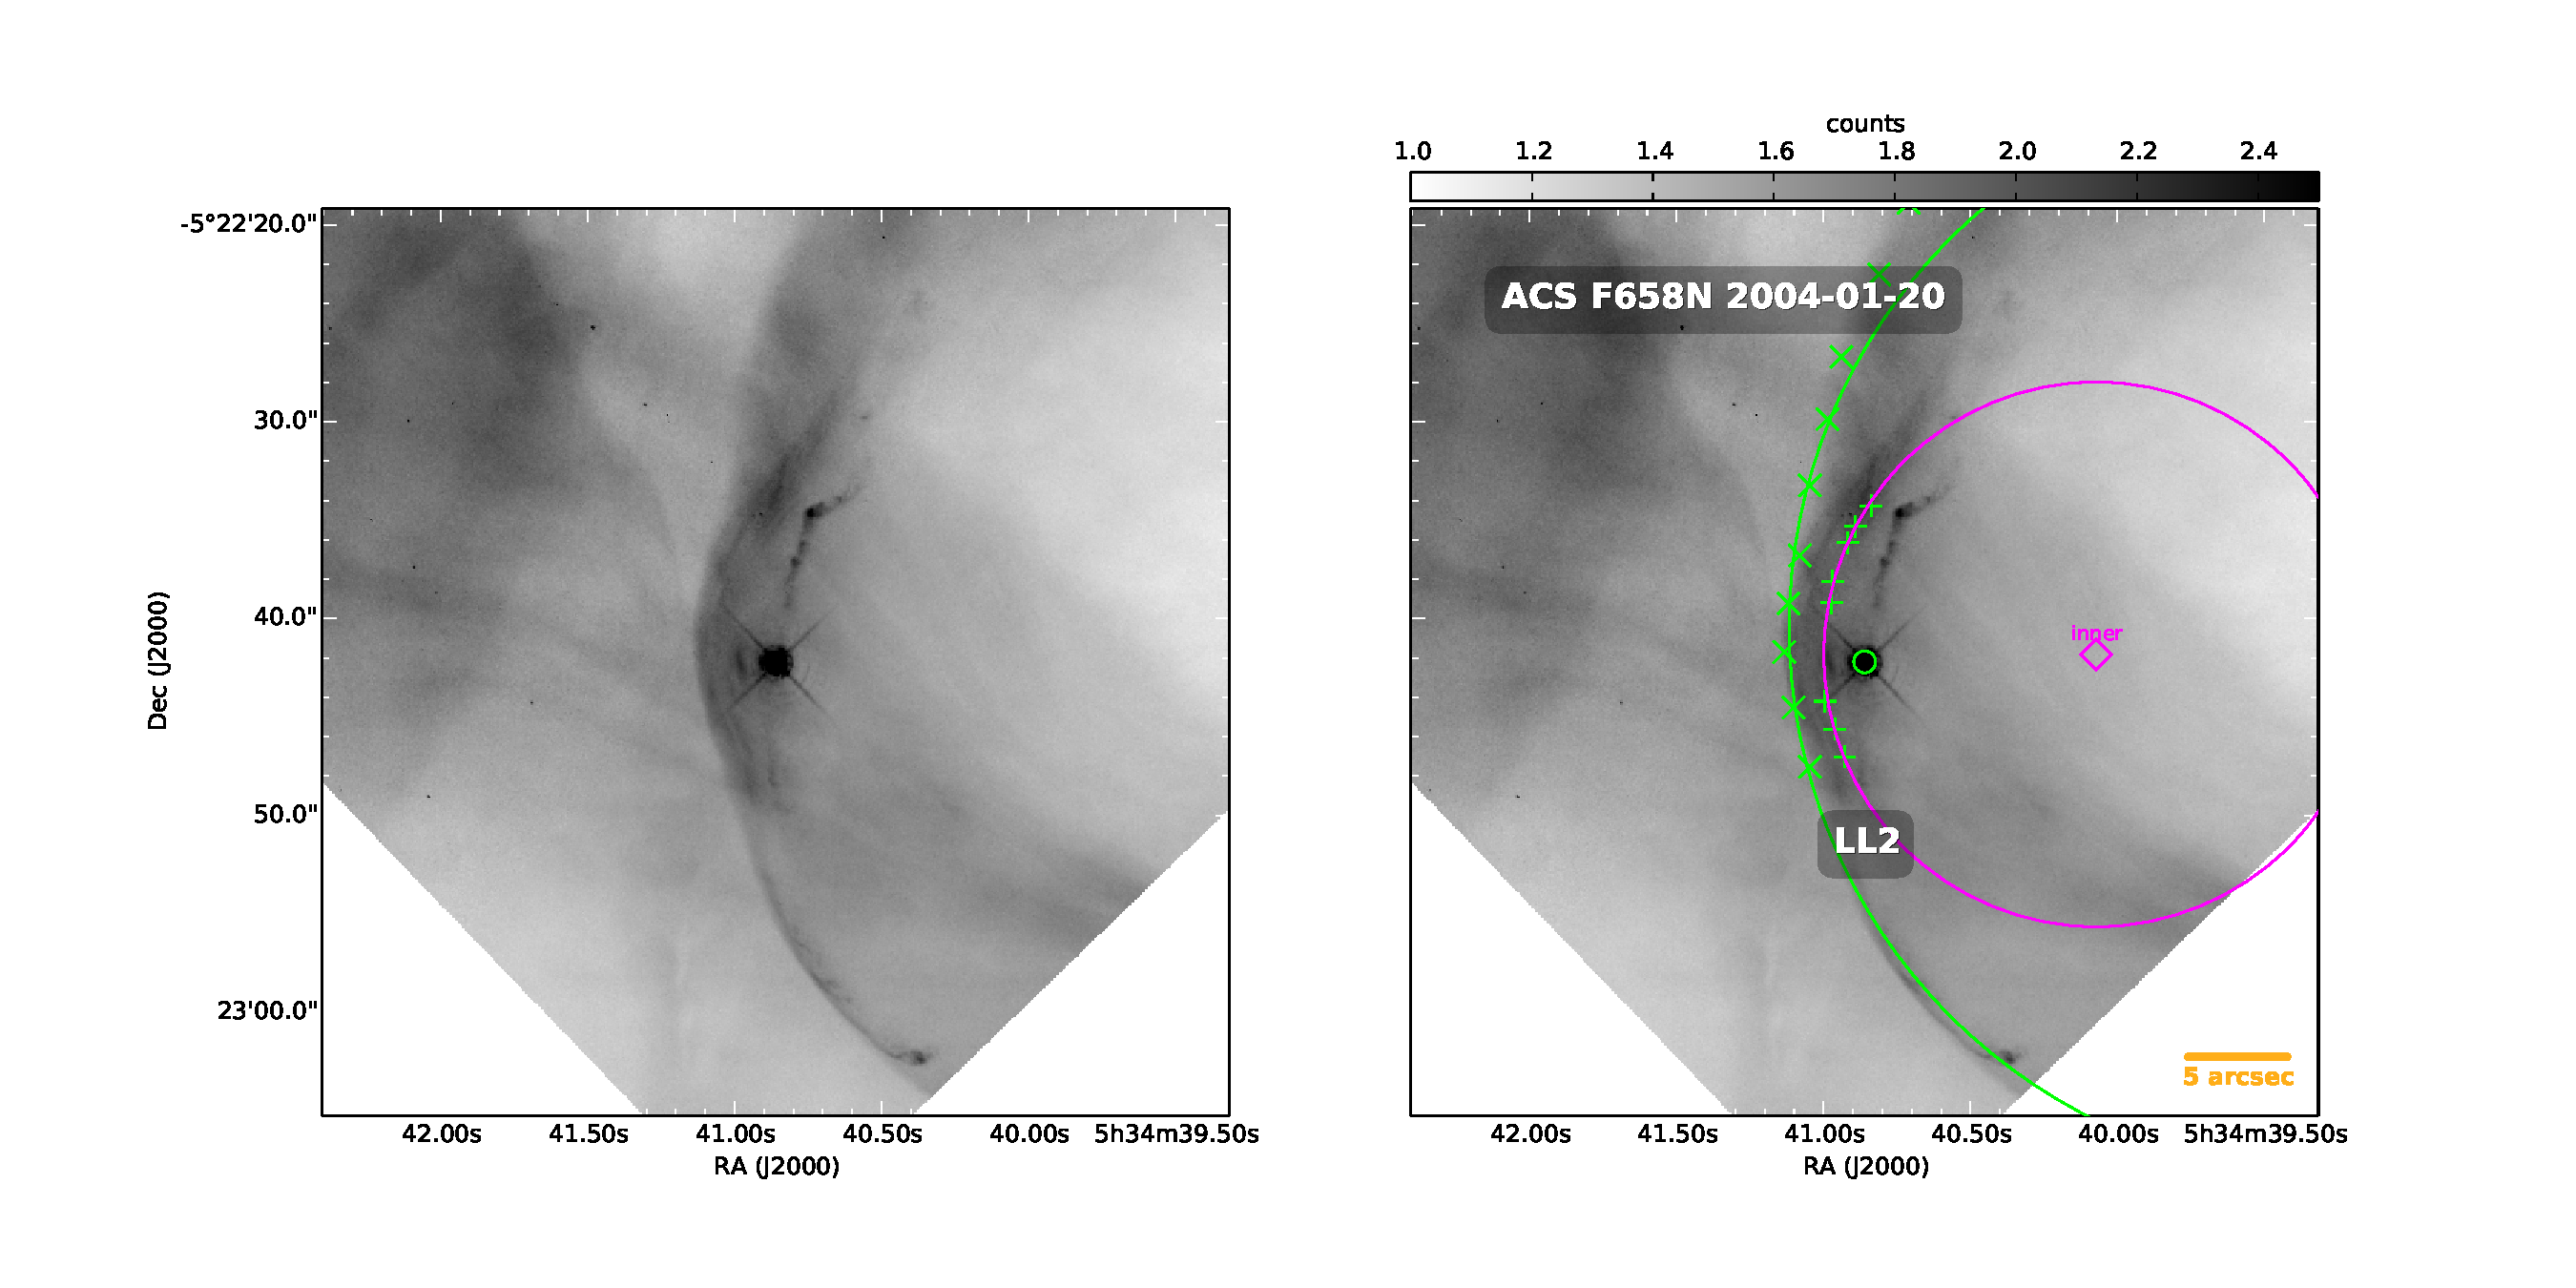
\includegraphics[width=\figwidth,  trim=60 50 100 50, clip]{j8oc18010_wcs/LL2-Bally_18-images.pdf}} 
   &\framebox{\includegraphics[width=\figwidth,  trim=60 50 100 50, clip]{j8oc17010_wcs/LL3-Bally_17-images.pdf}}\\ 
   \framebox{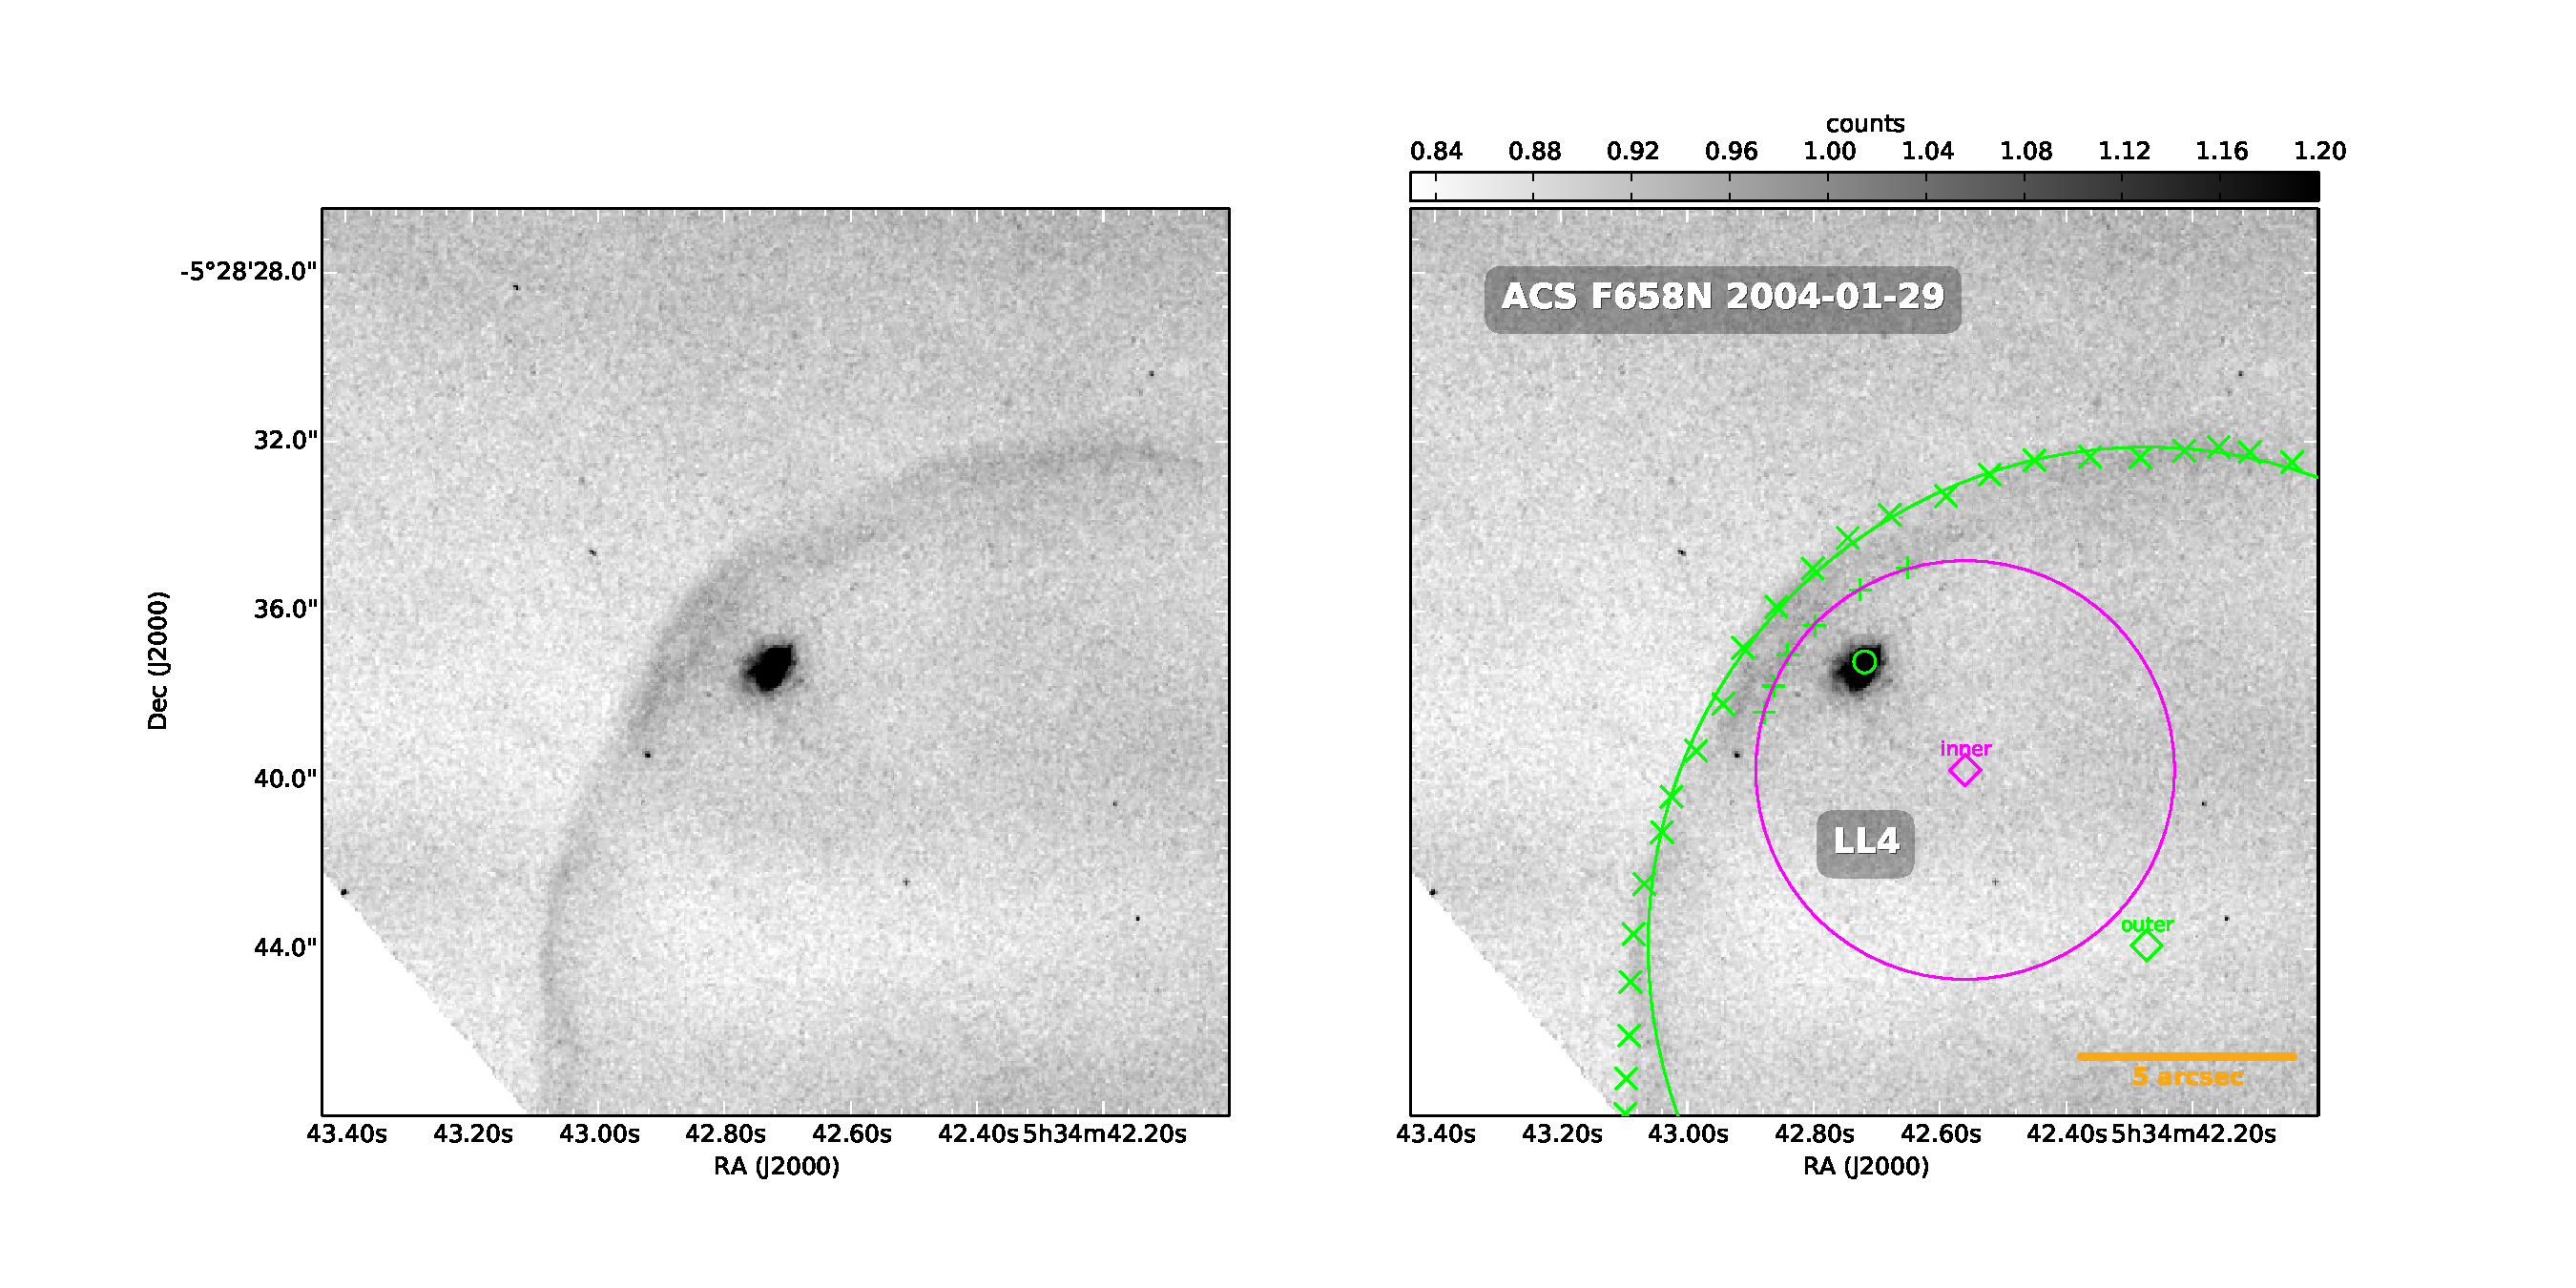
\includegraphics[width=\figwidth,  trim=60 50 100 50, clip]{j8oc24010_wcs/LL4-Bally_24-images.pdf}}
   &\framebox{\includegraphics[width=\figwidth,  trim=60 50 100 50, clip]{j8oc17010_wcs/4468-605-Bally_17-images.pdf}}\\
   \framebox{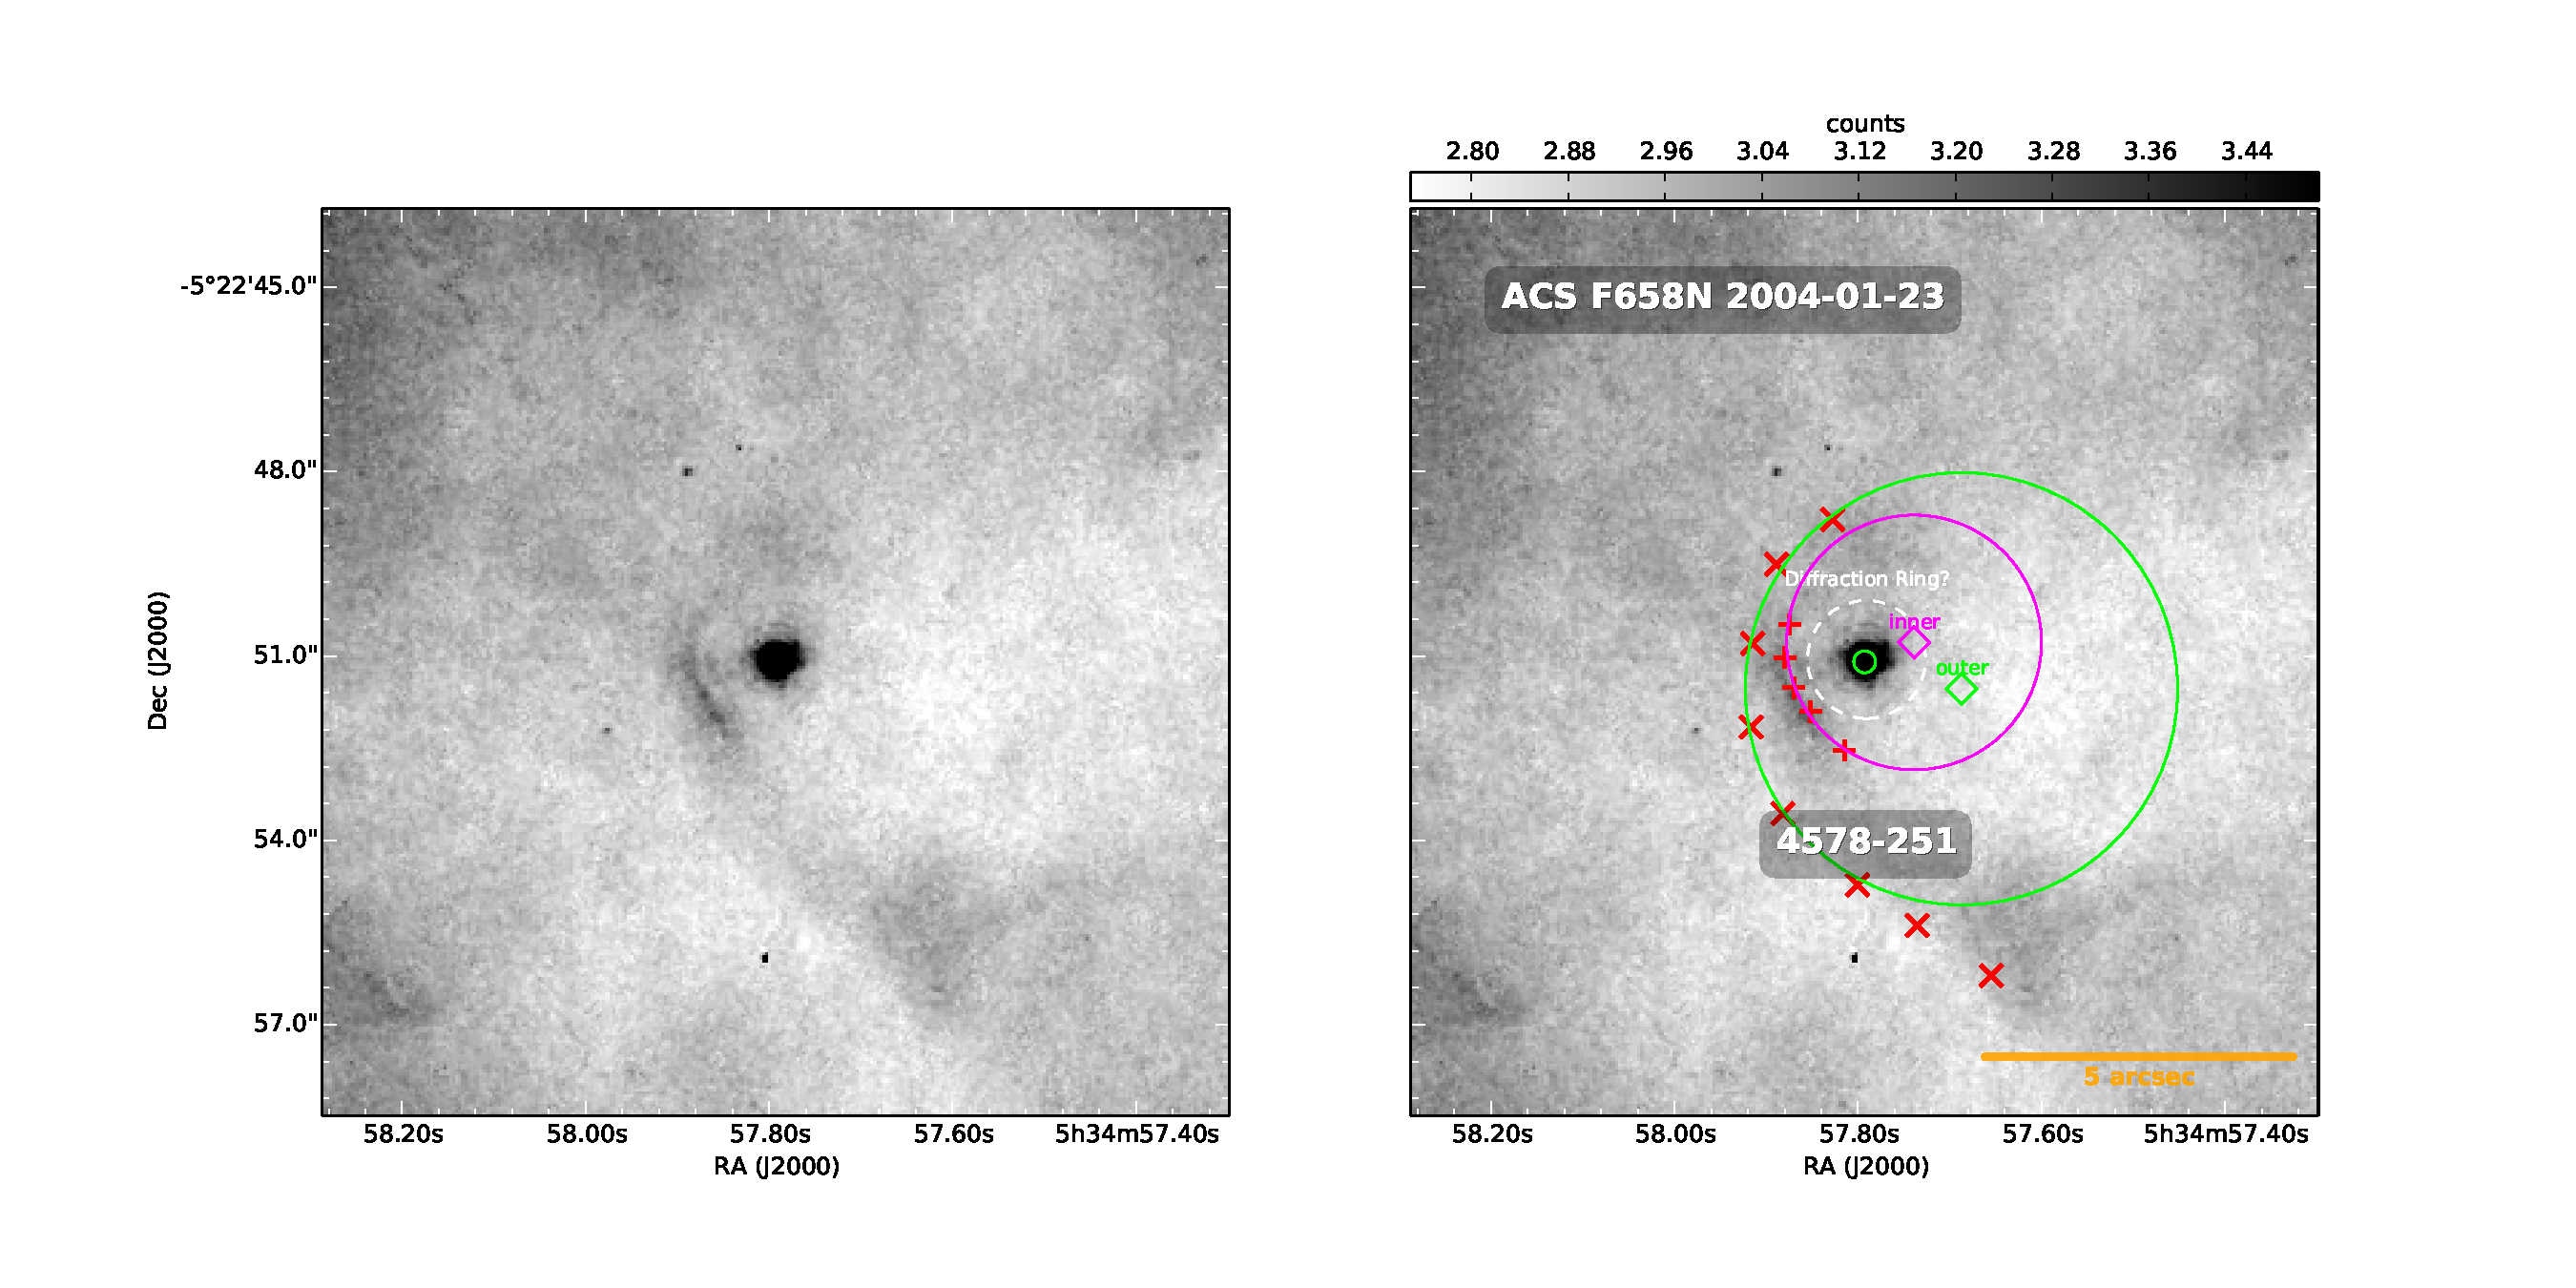
\includegraphics[width=\figwidth,  trim=60 50 100 50, clip]{j8oc09010_wcs/4578-251-Bally_09-images.pdf}}
   &\framebox{\includegraphics[width=\figwidth,  trim=60 50 100 50, clip]{j8oc16010_wcs/4582-635-Bally_16-images.pdf}}\\ 
    \framebox{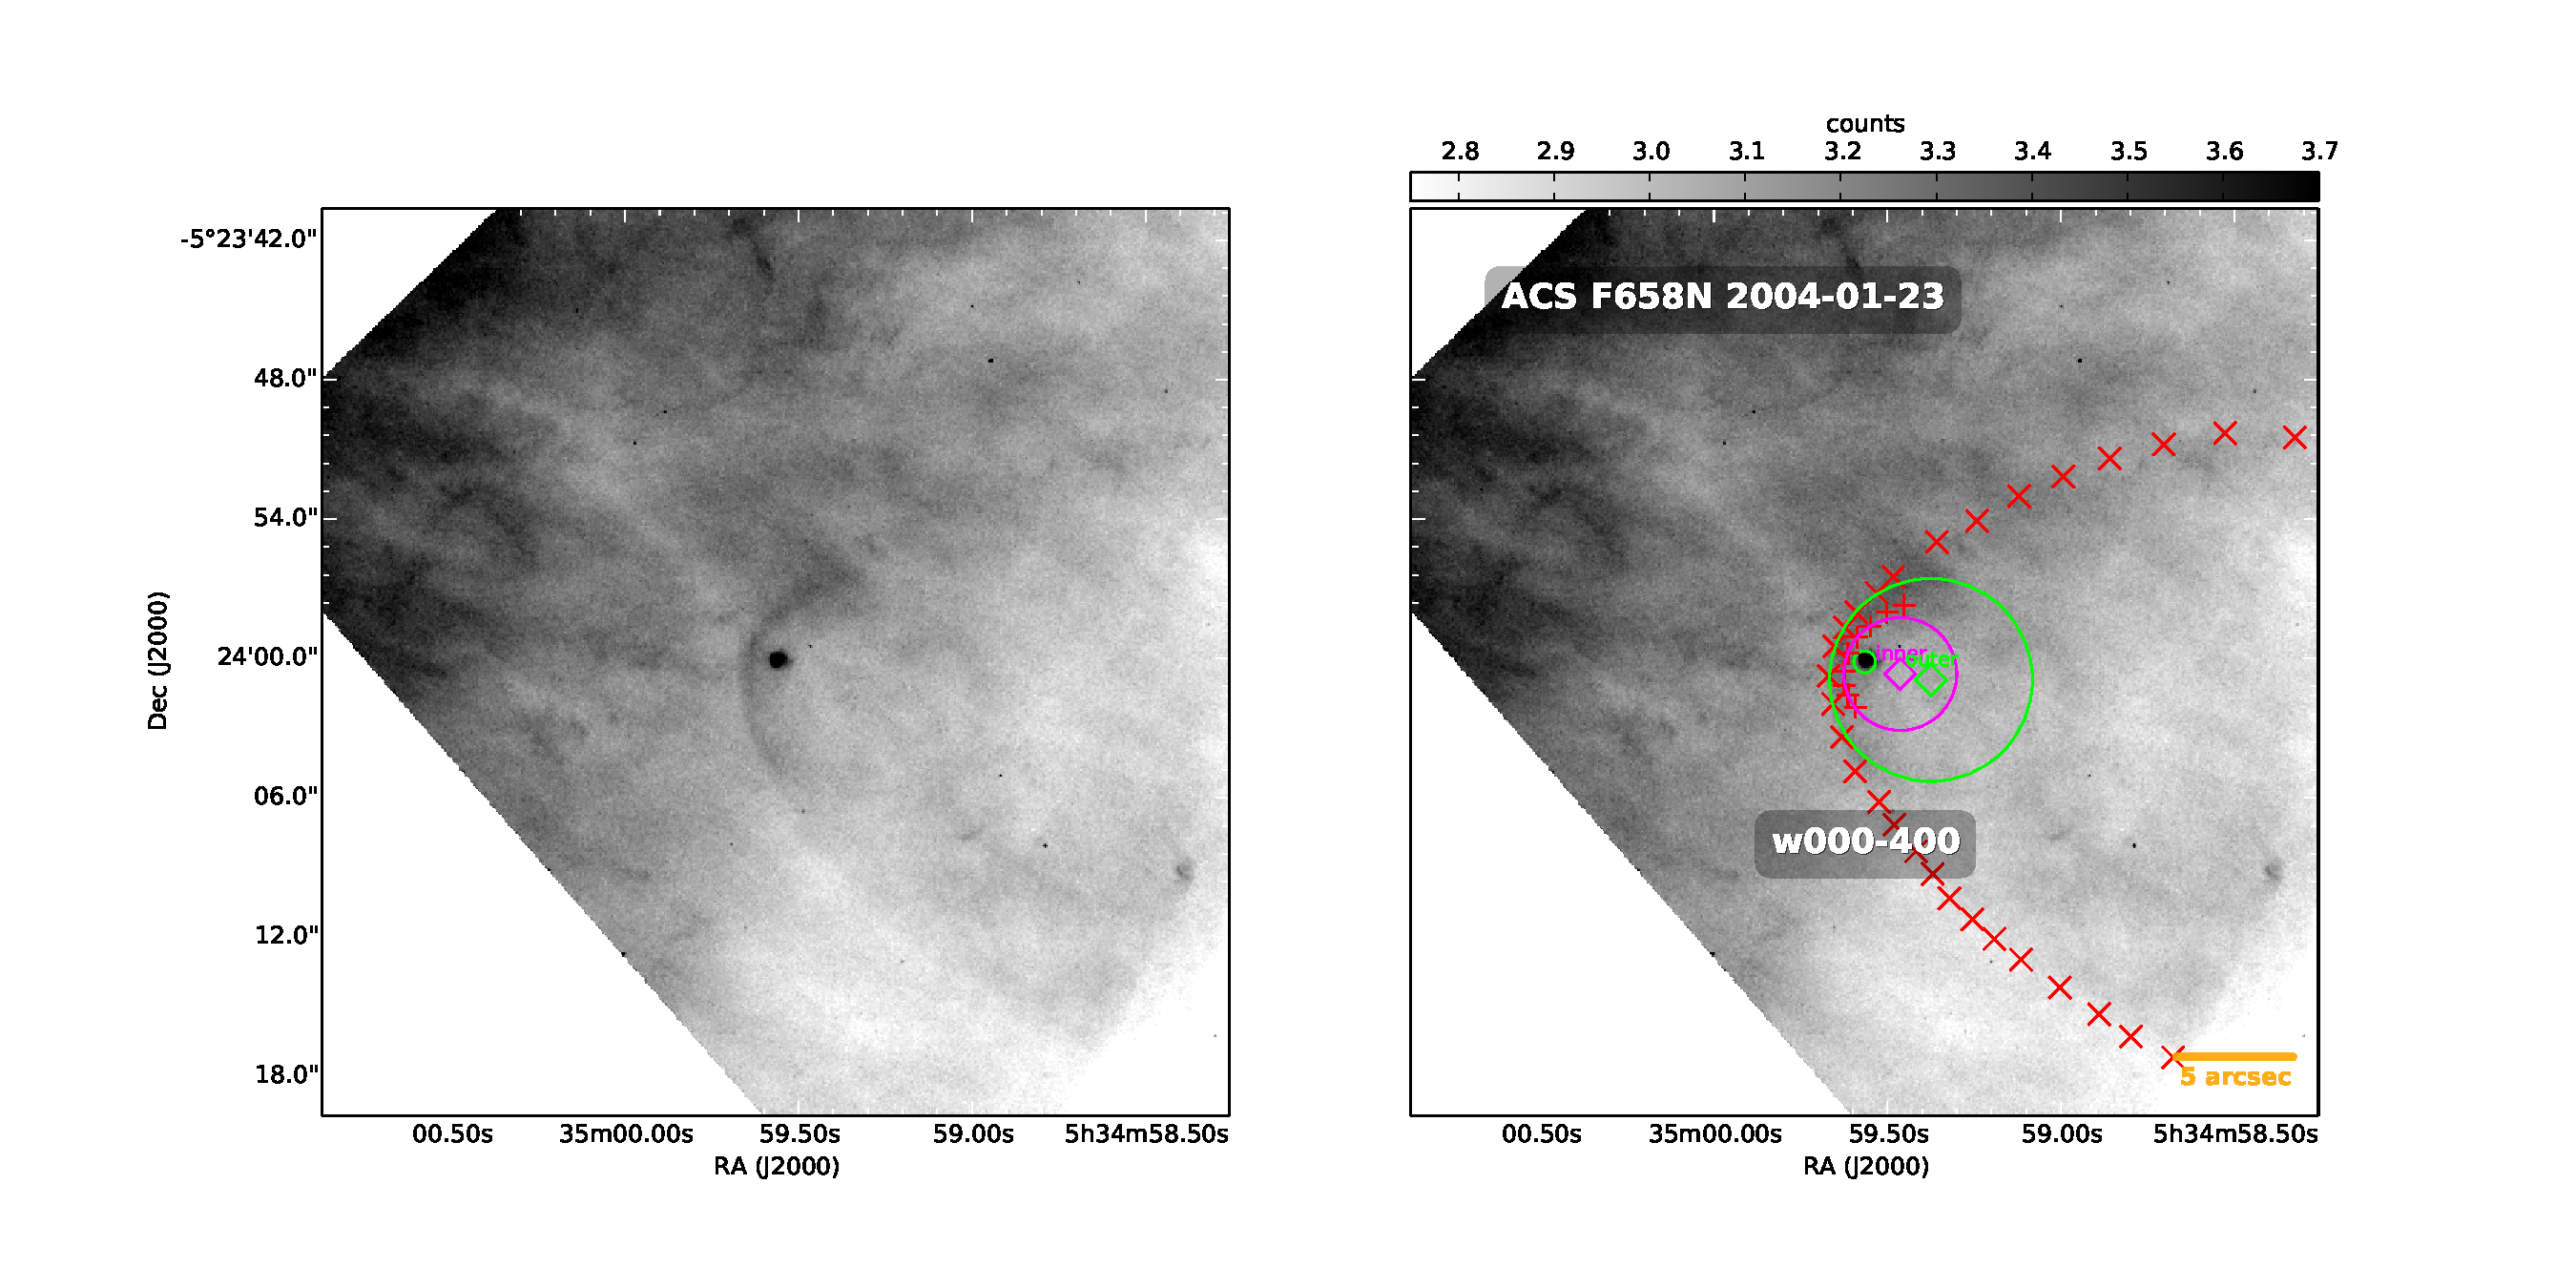
\includegraphics[width=\figwidth, trim=60 50 100 50, clip]{j8oc09010_wcs/w000-400-Bally_09-images.pdf}}
   &\framebox{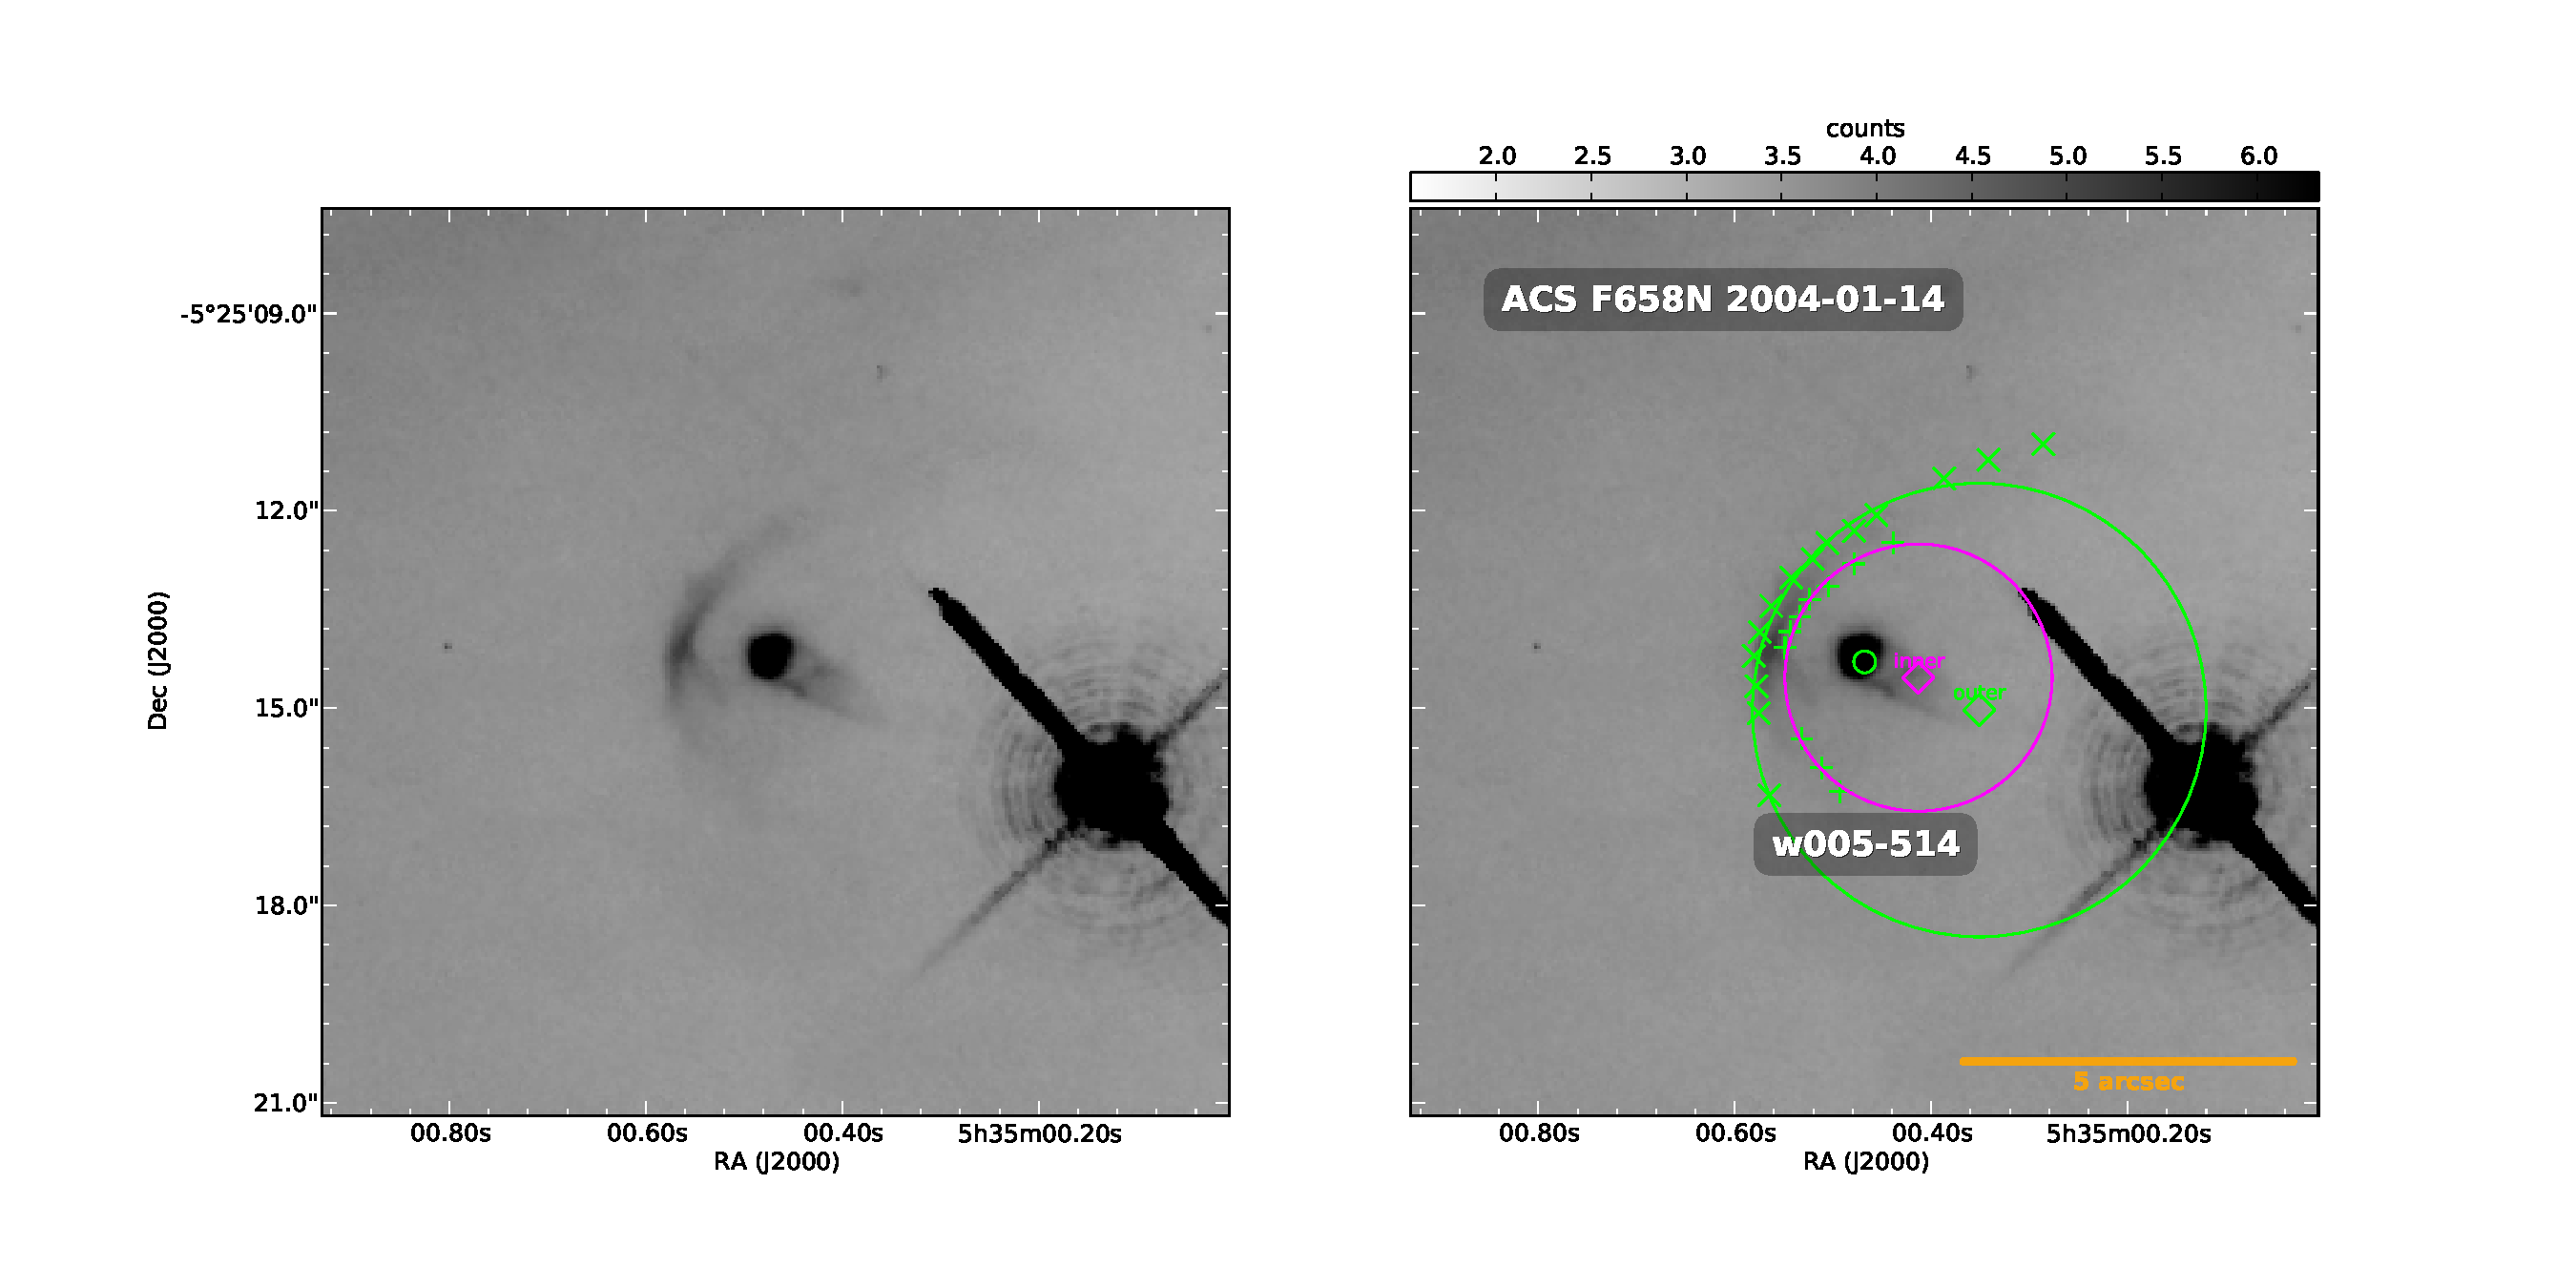
\includegraphics[width=\figwidth, trim=60 50 100 50, clip]{j8oc01010_wcs/w005-514-Bally_01-images.pdf}}\\  
   \framebox{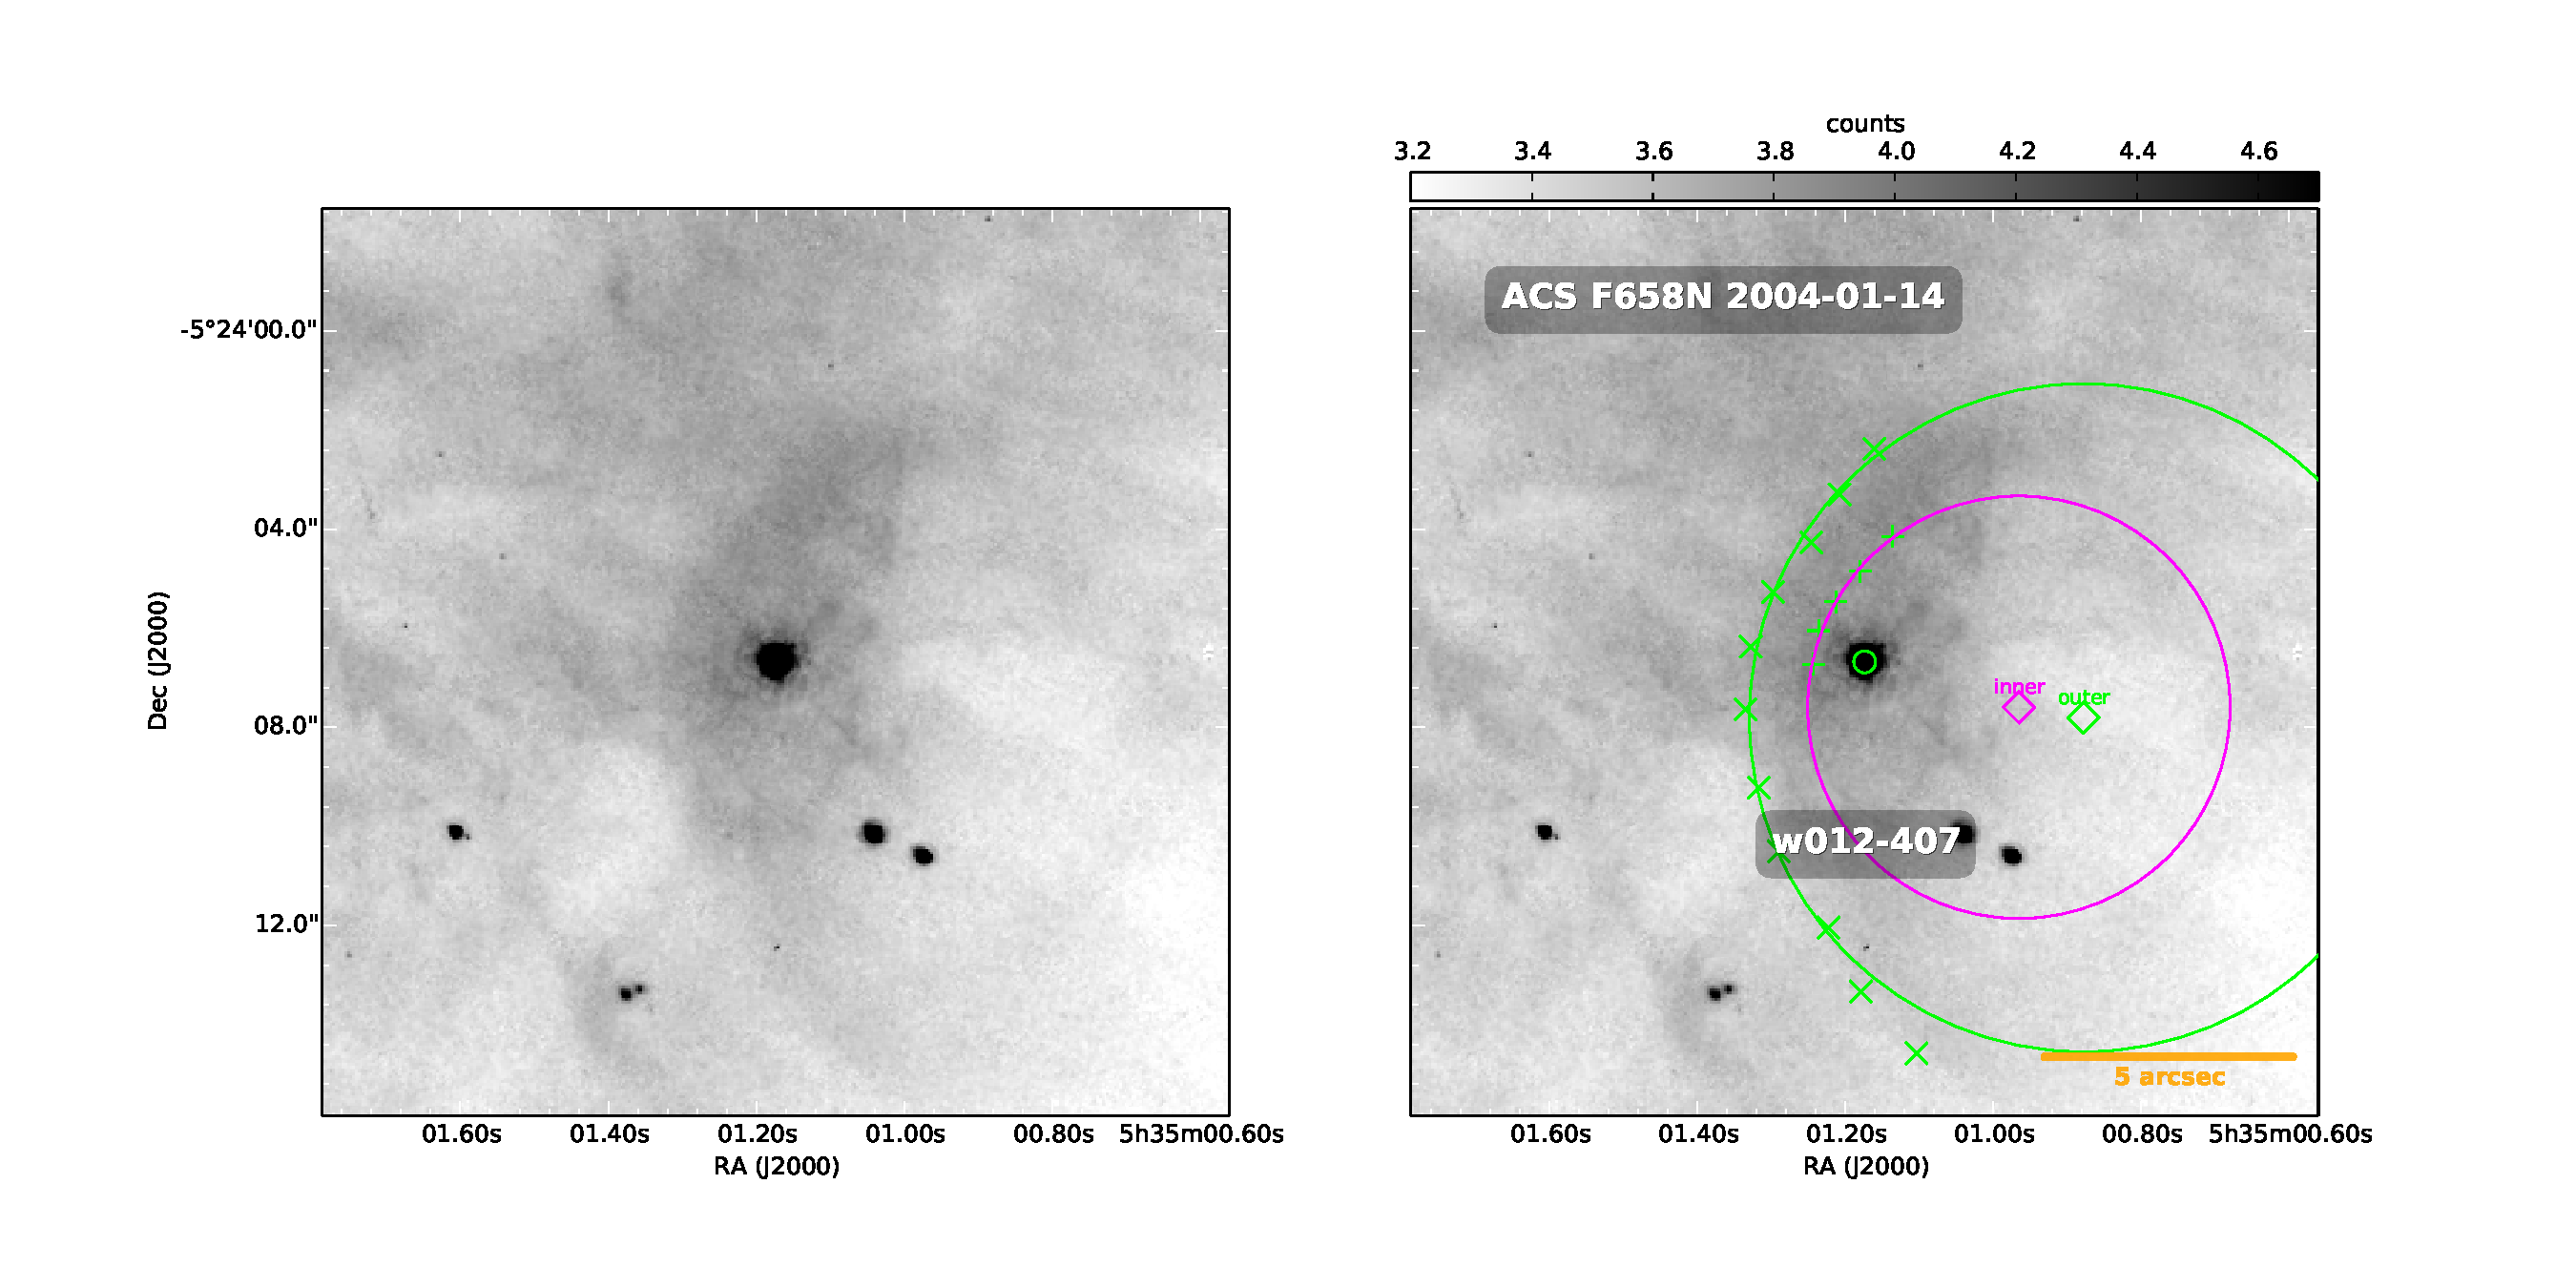
\includegraphics[width=\figwidth, trim=60 50 100 50, clip]{j8oc01010_wcs/w012-407-Bally_01-images.pdf}}
   &\framebox{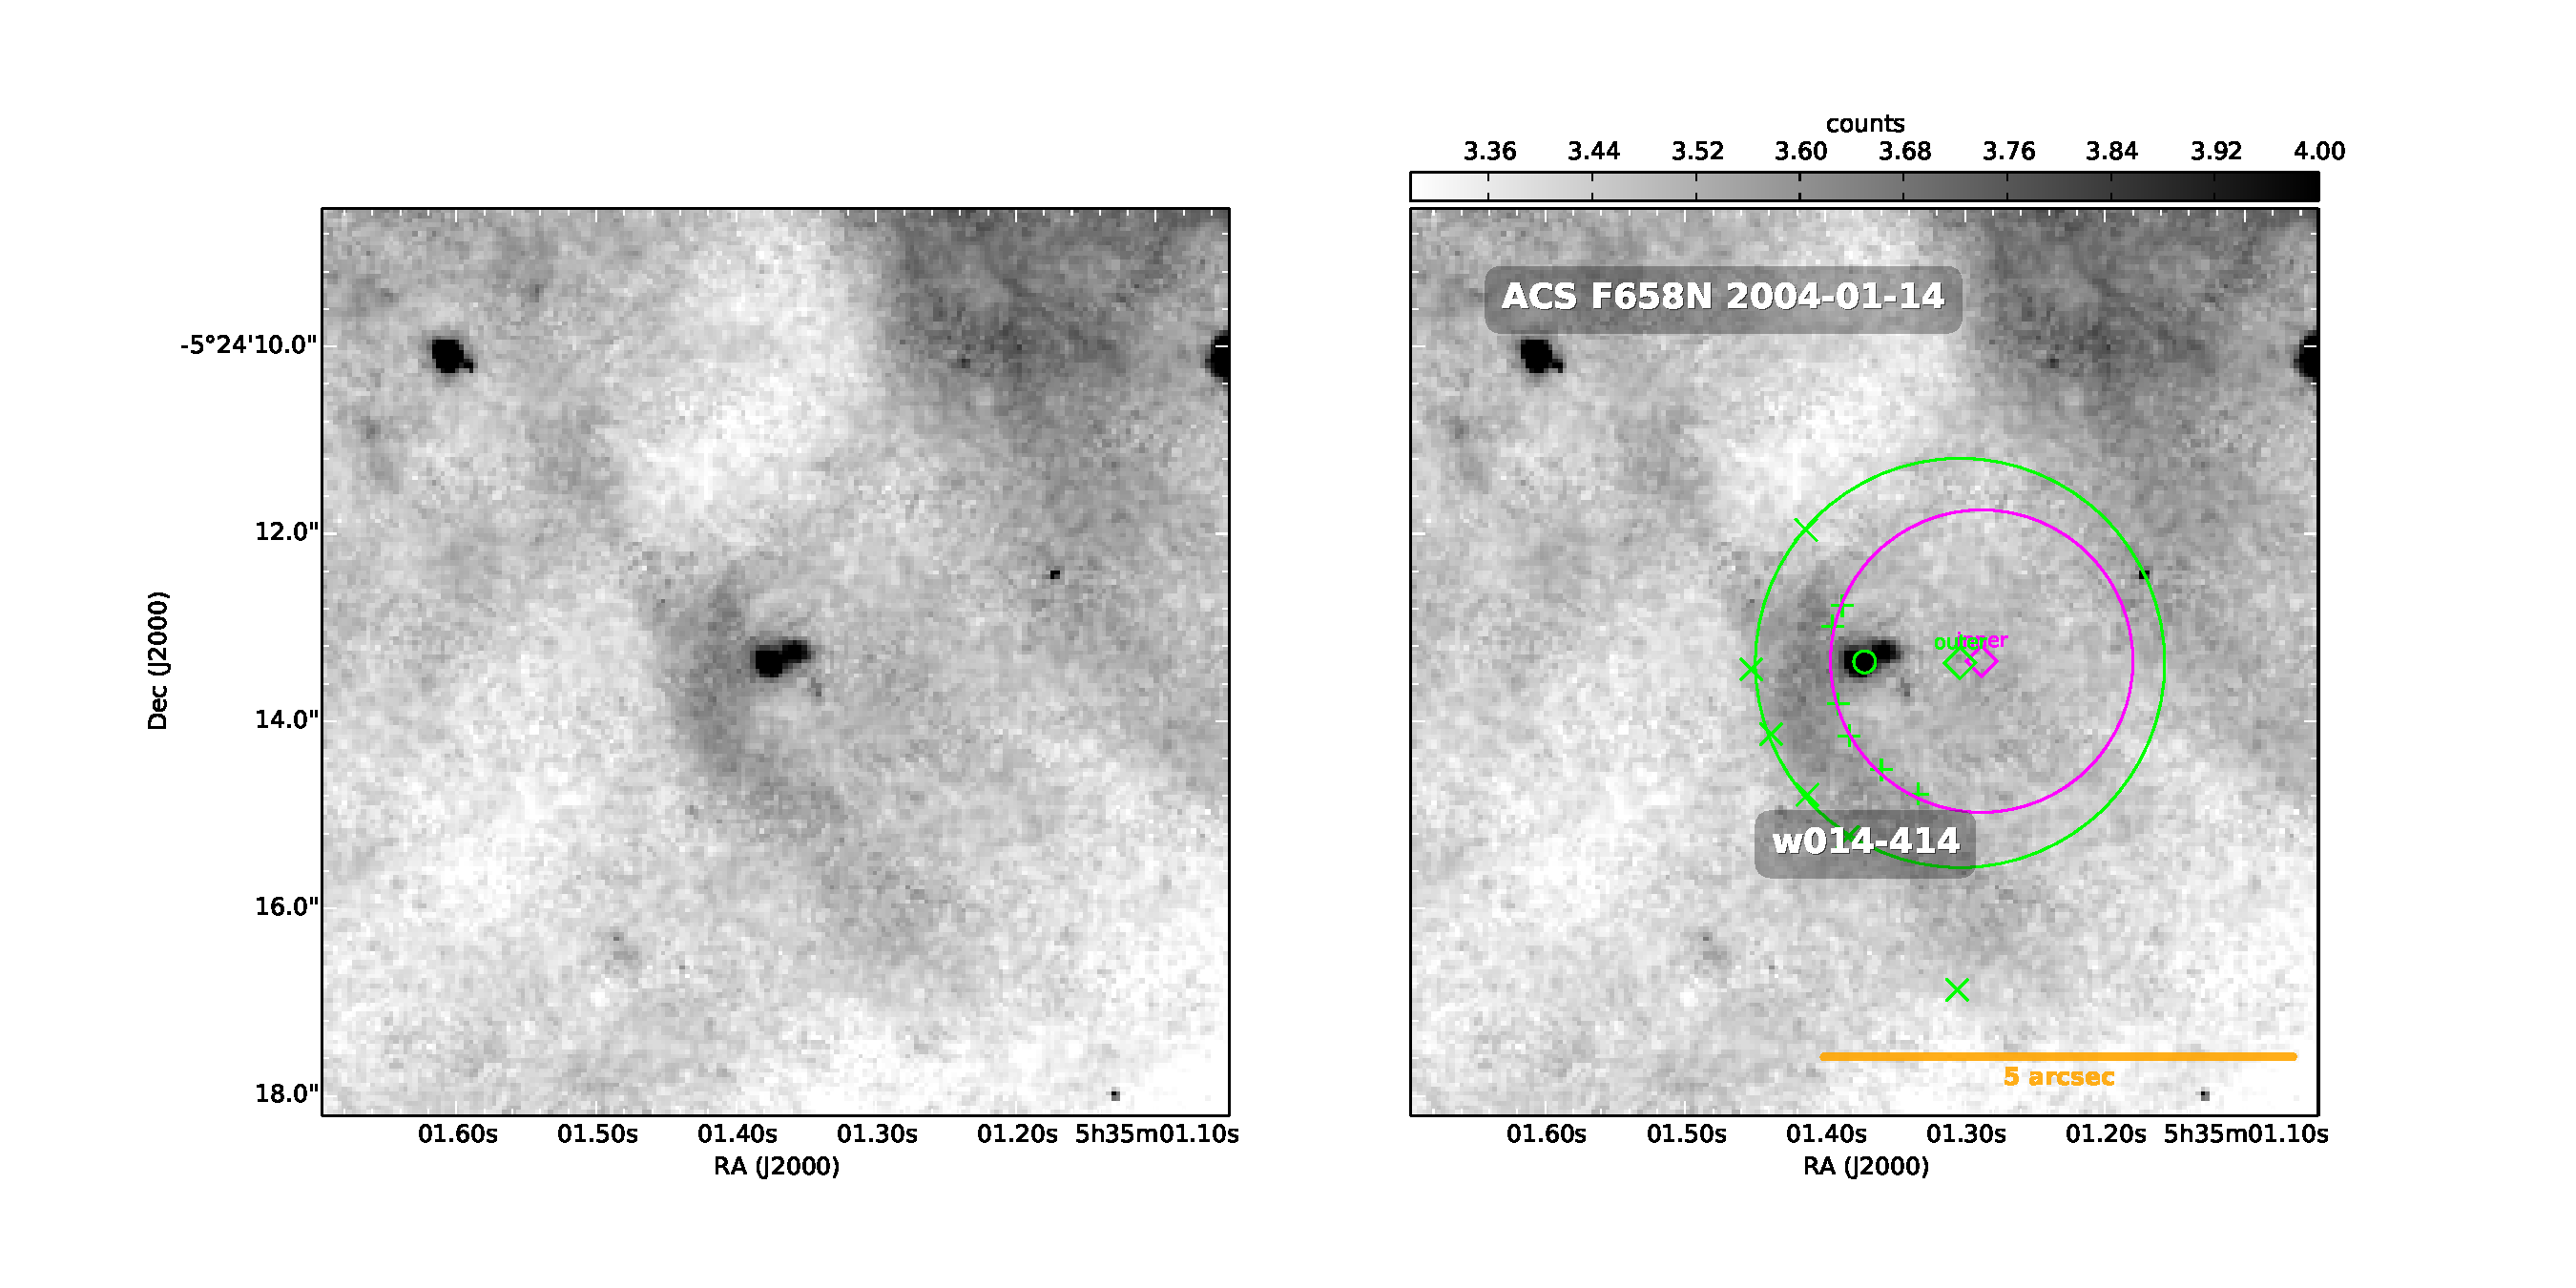
\includegraphics[width=\figwidth, trim=60 50 100 50, clip]{j8oc01010_wcs/w014-414-Bally_01-images.pdf}}\\ 
   \framebox{\includegraphics[width=\figwidth, trim=60 50 100 50, clip]{j8oc16010_wcs/022-635-Bally_16-images.pdf}}
   &\framebox{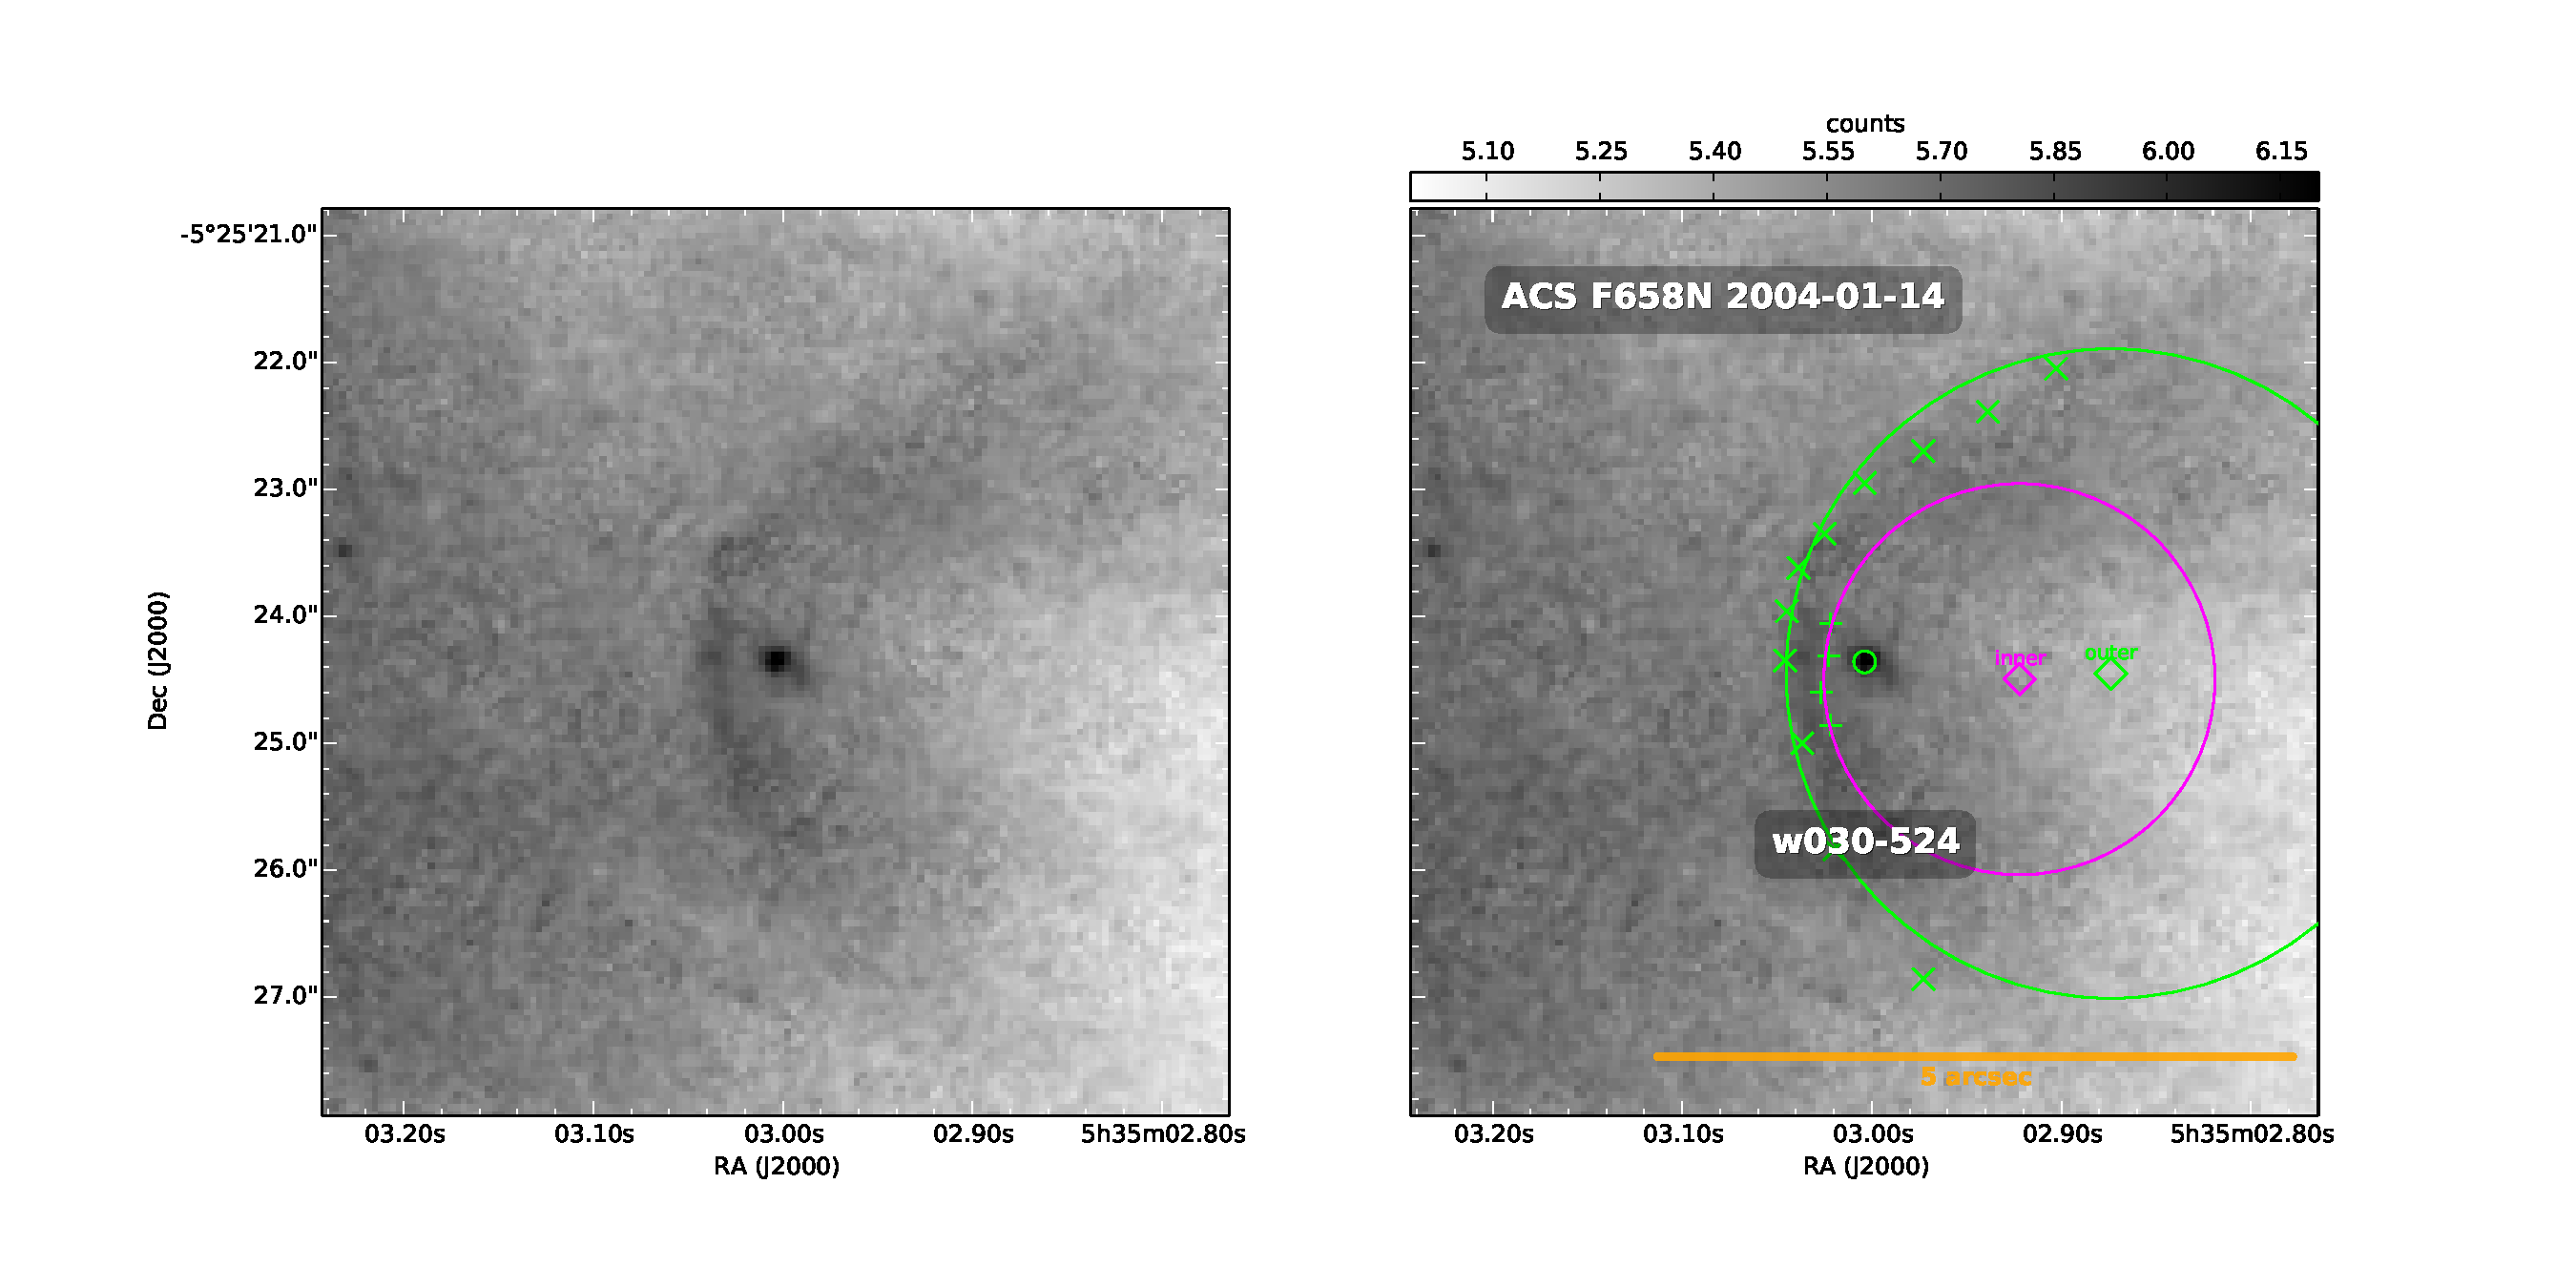
\includegraphics[width=\figwidth, trim=60 50 100 50, clip]{j8oc01010_wcs/w030-524-Bally_01-images.pdf}}\\ 
\end{tabular}
\end{figure*}

\begin{figure*}
\setlength\tabcolsep{1.5pt}
\begin{tabular}{l l}

   \framebox{\includegraphics[width=\figwidth,  trim=60 50 100 50, clip]{j8oc16010_wcs/041-637-Bally_16-images.pdf}}
   &\framebox{\includegraphics[width=\figwidth,  trim=60 50 100 50, clip]{j8oc16010_wcs/042-628-Bally_16-images.pdf}}\\ 
   \framebox{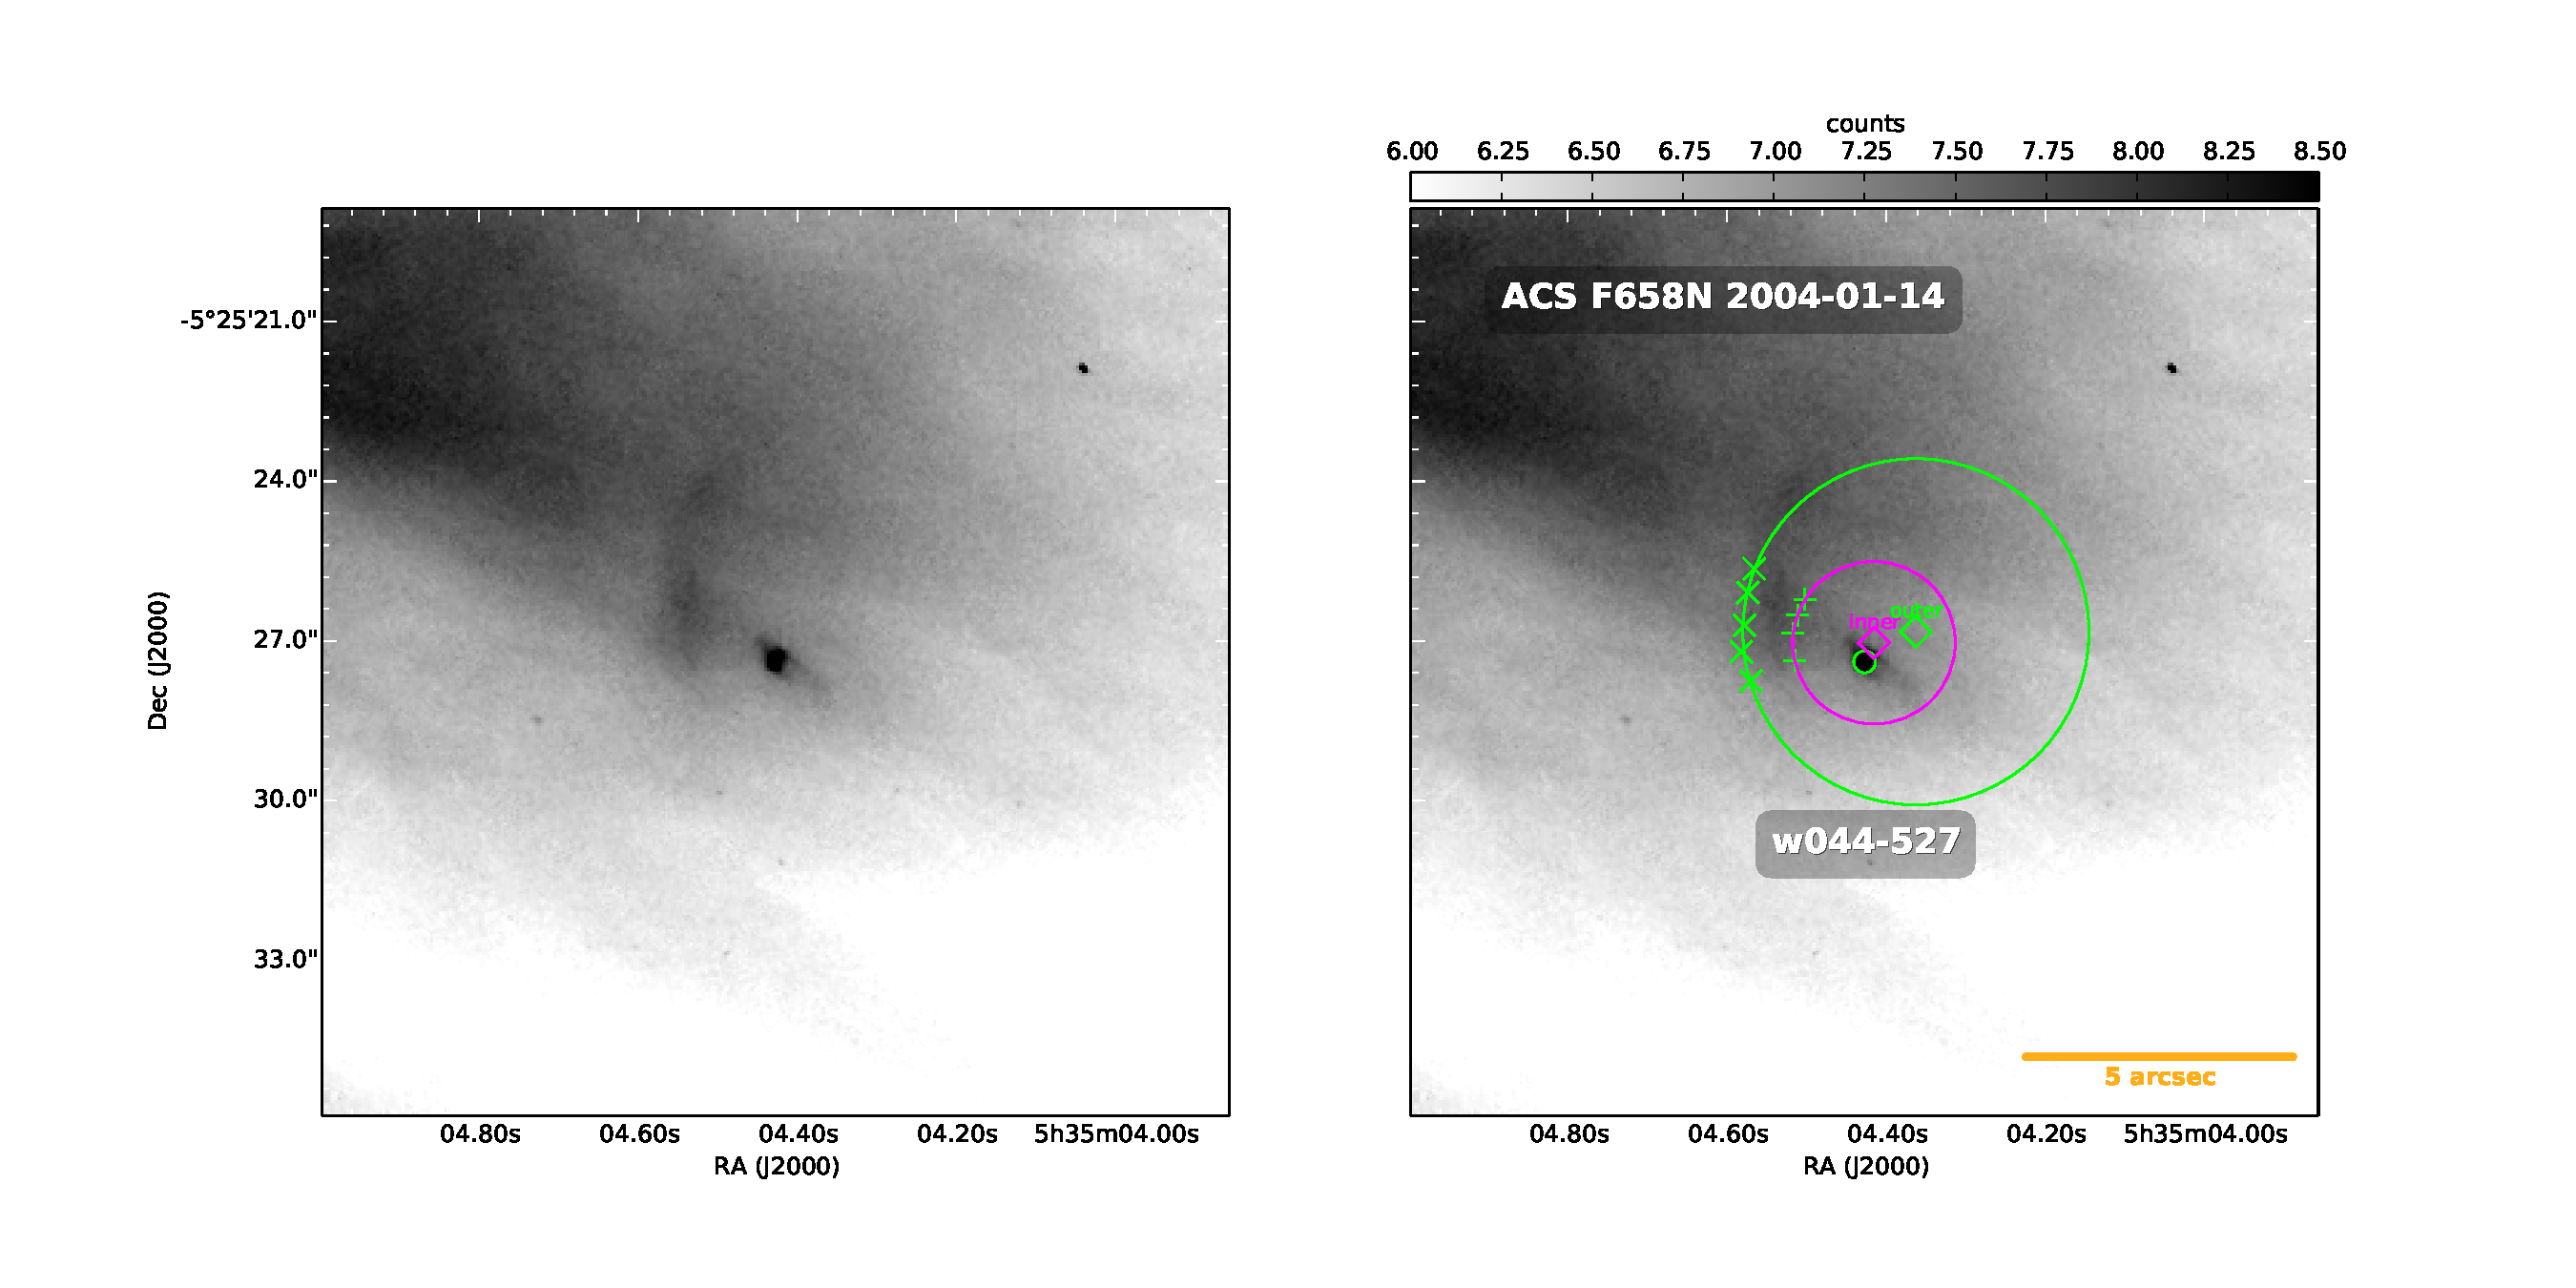
\includegraphics[width=\figwidth,  trim=60 50 100 50, clip]{j8oc01010_wcs/w044-527-Bally_01-images.pdf}}
   &\framebox{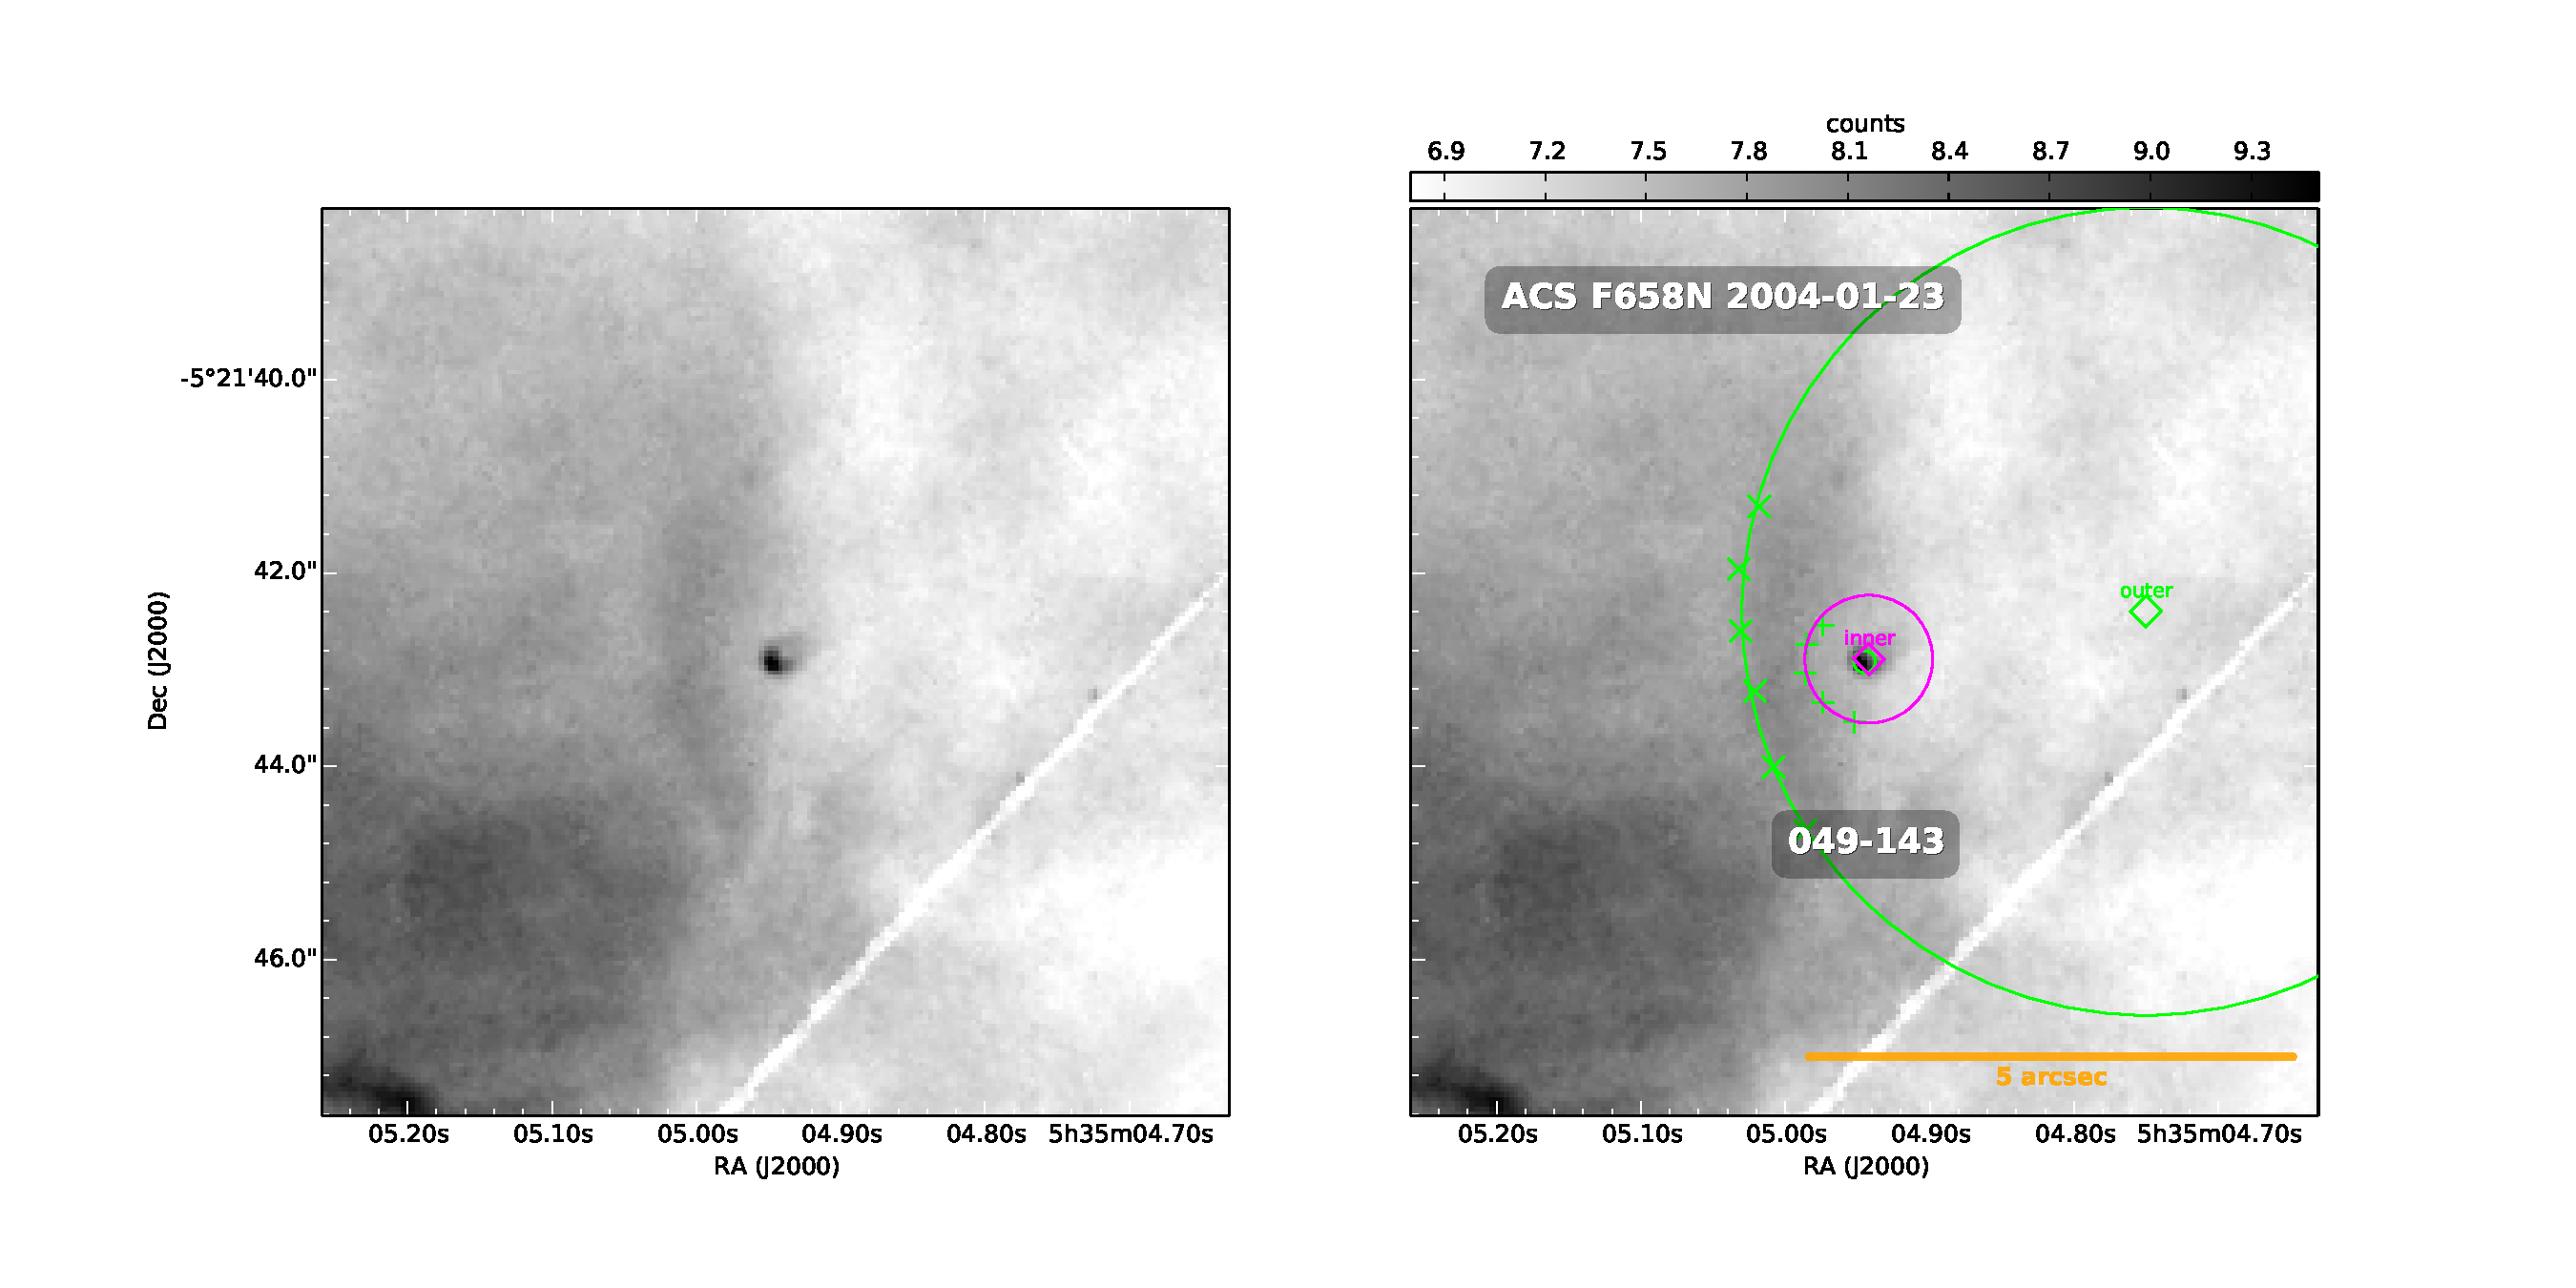
\includegraphics[width=\figwidth,  trim=60 50 100 50, clip]{j8oc09010_wcs/049-143-Bally_09-images.pdf}}\\ 
   \framebox{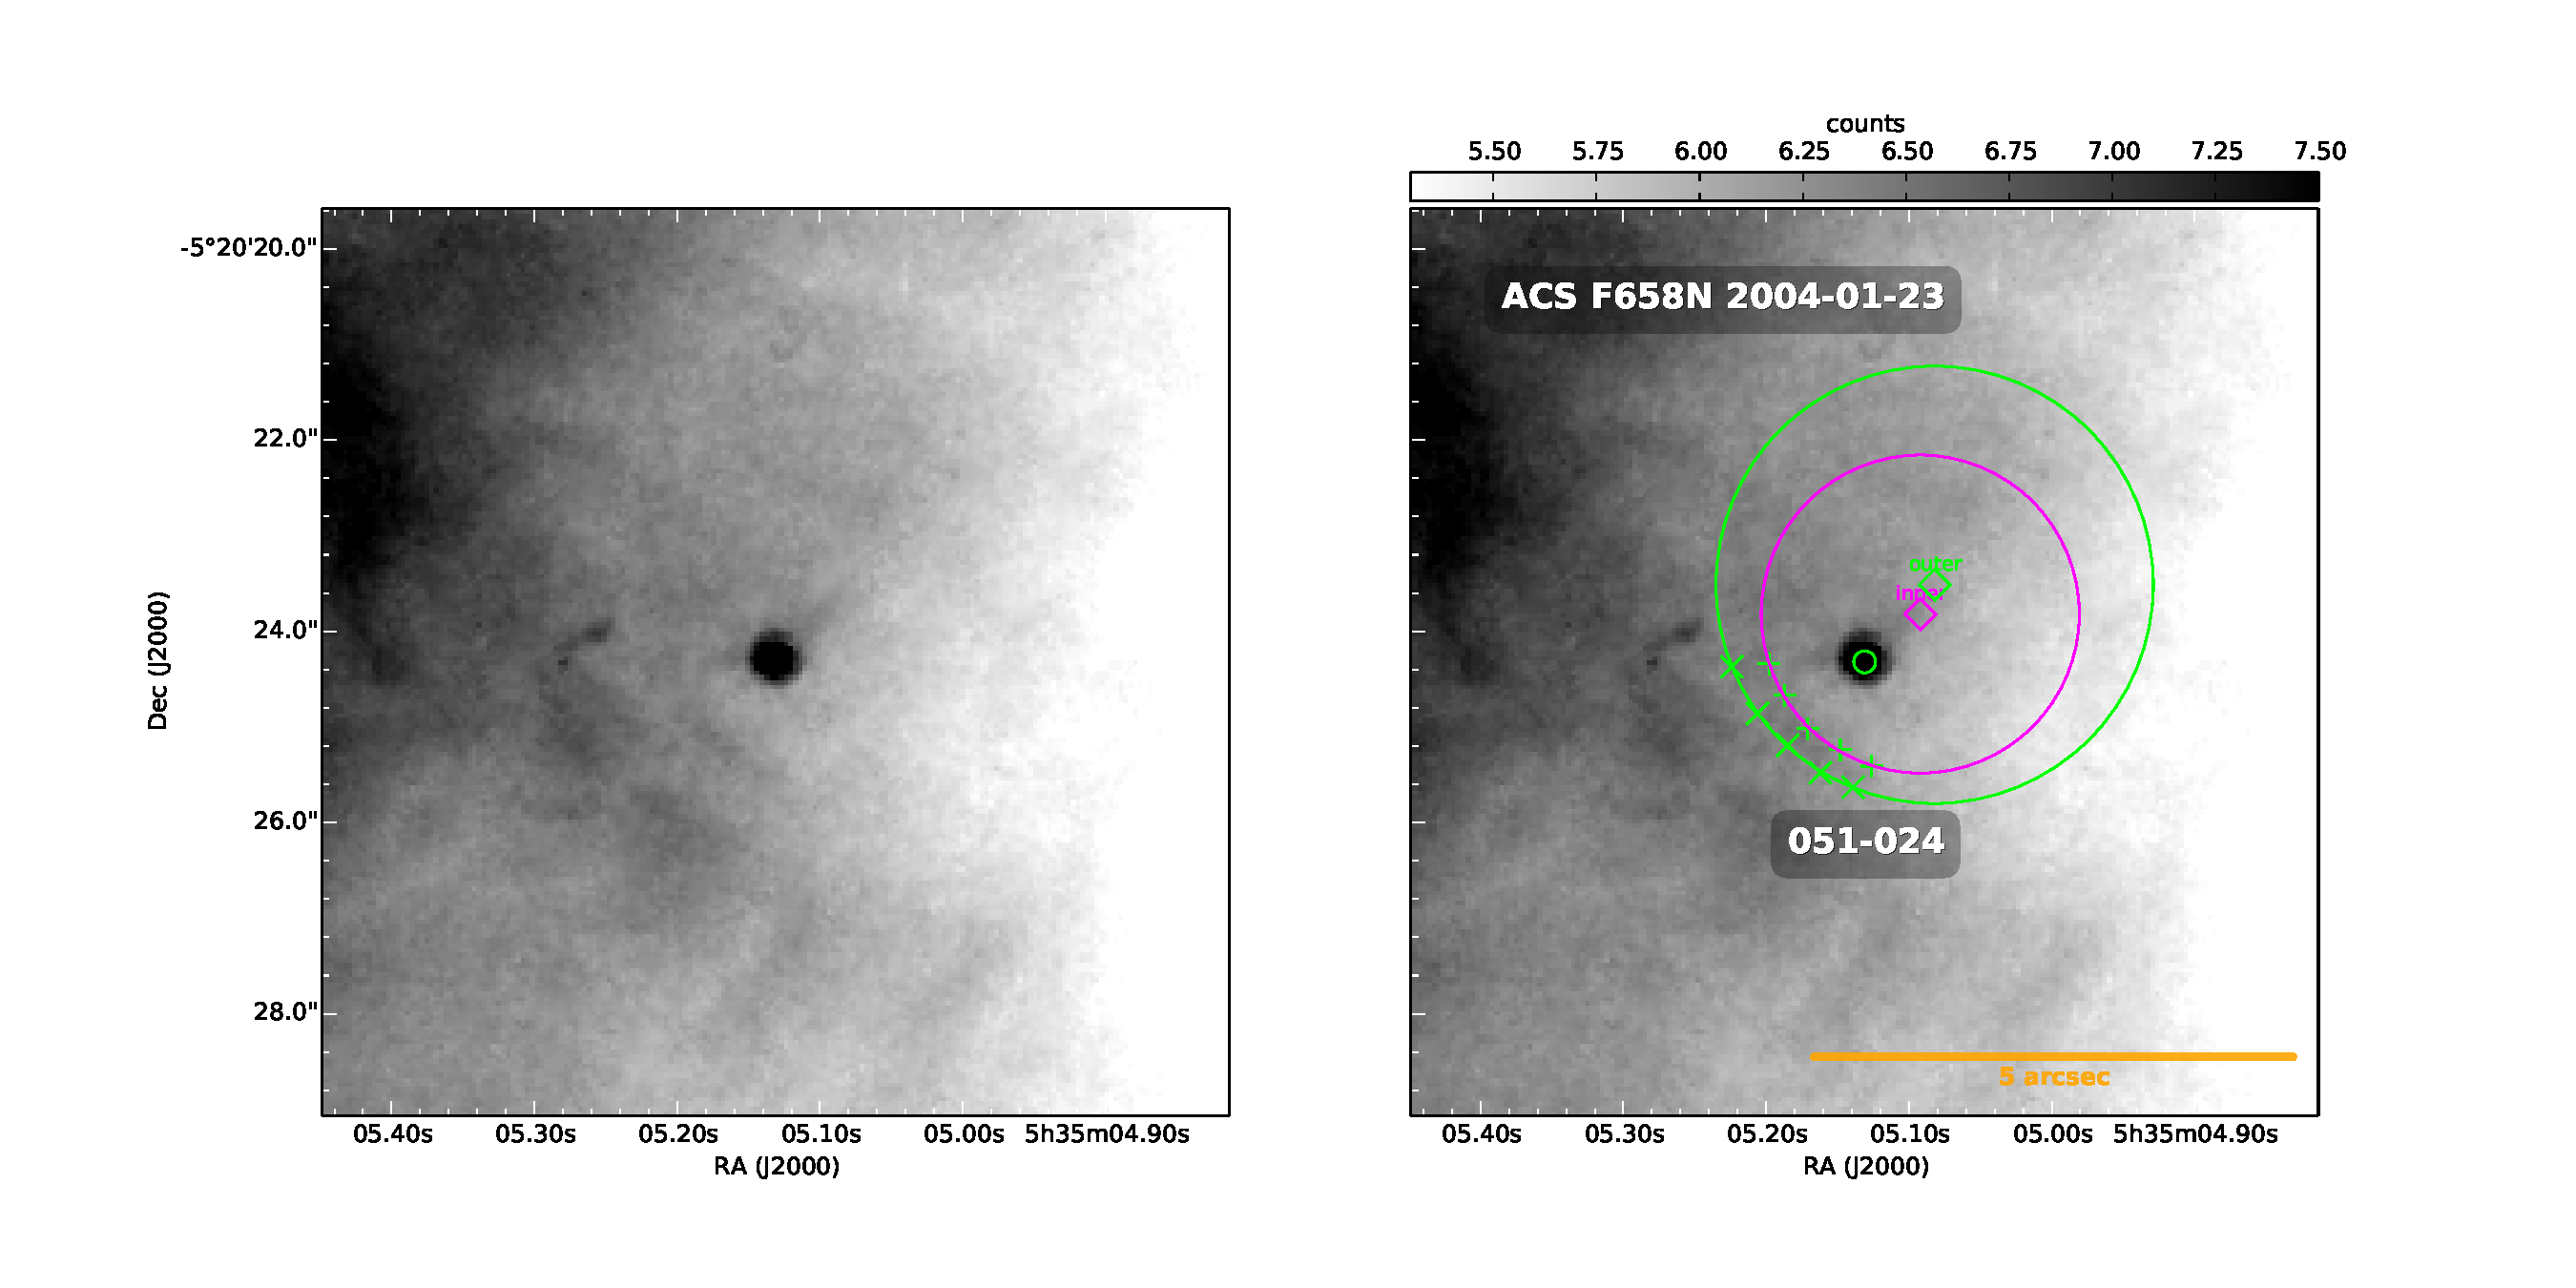
\includegraphics[width=\figwidth,  trim=60 50 100 50, clip]{j8oc09010_wcs/051-024-Bally_09-images.pdf}}
   &\framebox{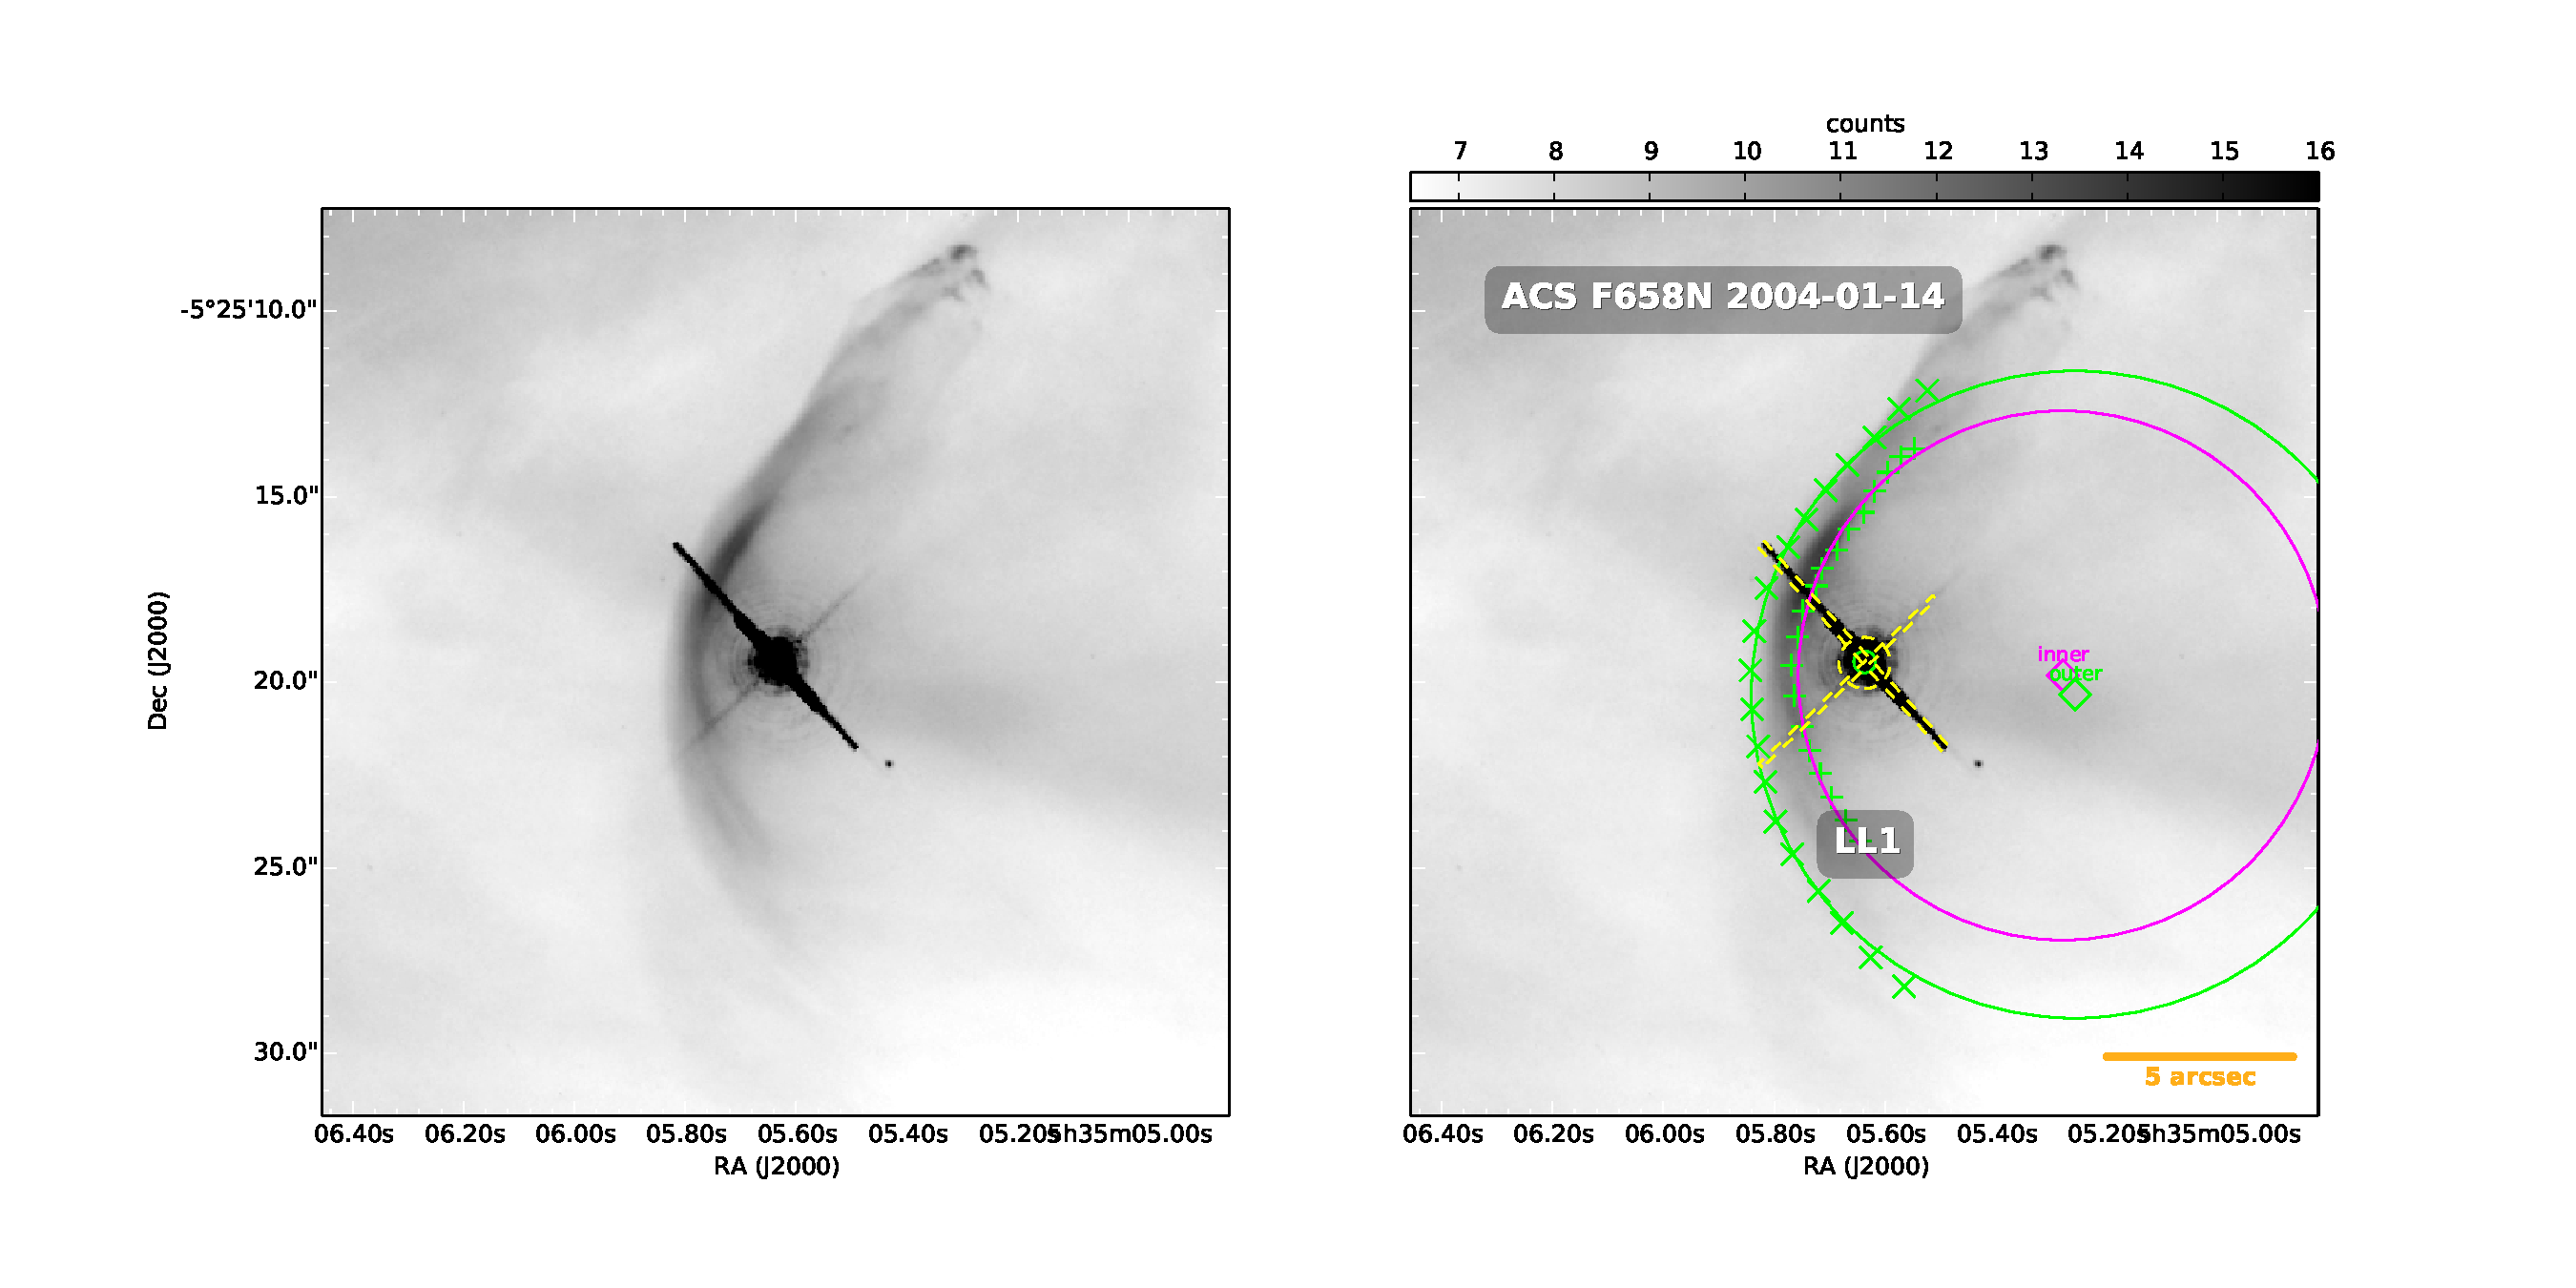
\includegraphics[width=\figwidth,  trim=60 50 100 50, clip]{j8oc01010_wcs/LL1-Bally_01-images.pdf}}\\ 
    \framebox{\includegraphics[width=\figwidth,  trim=60 50 100 50, clip]{j8oc01010_wcs/065-502-Bally_01-images.pdf}}
    %\includegraphics[width=0.47\linewidth,  trim=60 50 100 50, clip]{j8oc06010_wcs/066-652-Bally_06-images.pdf}%
   &\framebox{\includegraphics[width=\figwidth,  trim=60 50 90 50, clip]{j8oc14010_wcs/066-3251-Bally_14-images.pdf}}\\ 
   \framebox{\includegraphics[width=\figwidth,  trim=60 50 100 50, clip]{j8oc01010_wcs/w069-601-Bally_01-images.pdf}}
   &\framebox{\includegraphics[width=\figwidth,  trim=60 50 100 50, clip]{j8oc09010_wcs/072-134-Bally_09-images.pdf}}\\ 
   \framebox{\includegraphics[width=\figwidth,  trim=60 50 100 50, clip]{j8oc01010_wcs/w073-227-Bally_01-images.pdf}}
 &\framebox{\includegraphics[width=\figwidth,  trim=60 50 100 50, clip]{j8oc01010_wcs/074-229-Bally_01-images.pdf}}\\ 
\end{tabular}
\end{figure*} 

\begin{figure*}
\setlength\tabcolsep{1.5pt}
\begin{tabular}{l l} 
  \framebox{\includegraphics[width=\figwidth,  trim=60 50 100 50, clip]{j8oc01010_wcs/083-435-Bally_01-images.pdf}}
    &\framebox{\includegraphics[width=\figwidth,  trim=60 50 100 50, clip]{j8oc01010_wcs/101-233-Bally_01-images.pdf}}\\
   \framebox{\includegraphics[width=\figwidth,  trim=60 50 100 50, clip]{j8oc01010_wcs/102-157-Bally_01-images.pdf}}
   &\framebox{\includegraphics[width=\figwidth,  trim=60 50 100 50, clip]{j8oc01010_wcs/106-245-Bally_01-images.pdf}}\\
   \framebox{\includegraphics[width=\figwidth,  trim=60 50 100 50, clip]{j8oc01010_wcs/109-246-Bally_01-images.pdf}}
  & \framebox{\includegraphics[width=\figwidth,  trim=60 50 100 50, clip]{j8oc14010_wcs/116-3101-Bally_14-images.pdf}}\\
   \framebox{\includegraphics[width=\figwidth,  trim=60 50 100 50, clip]{j8oc01010_wcs/117-421-Bally_01-images.pdf}}
   &\framebox{\includegraphics[width=\figwidth,  trim=60 50 100 50, clip]{j8oc14010_wcs/119-3155-Bally_14-images.pdf}}\\
   \framebox{\includegraphics[width=\figwidth,  trim=60 50 100 50, clip]{j8oc01010_wcs/121-434-Bally_01-images.pdf}}
%   \includegraphics[width=0.47\linewidth,  trim=60 50 100 50, clip]{j8oc01010_wcs/124-131-Bally_01-images.pdf}
   &\framebox{\includegraphics[width=\figwidth,  trim=60 50 100 50, clip]{j8oc02010_wcs/131-046-Bally_02-images.pdf}}\\
   \framebox{\includegraphics[width=\figwidth,  trim=60 50 100 50, clip]{j8oc02010_wcs/132-053-Bally_02-images.pdf}}
   & \framebox{\includegraphics[width=\figwidth,  trim=60 50 100 50, clip]{j8oc14010_wcs/136-3057-Bally_14-images.pdf}}\\
\end{tabular}
\end{figure*}   

\begin{figure*}
\setlength\tabcolsep{1.5pt}
\begin{tabular}{l l}
 \framebox{\includegraphics[width=\figwidth,  trim=60 50 100 50, clip]{j8oc14010_wcs/138-3024-Bally_14-images.pdf}}
   &\framebox{\includegraphics[width=\figwidth,  trim=60 50 100 50, clip]{j8oc01010_wcs/142-301-Bally_01-images.pdf}}\\
   \framebox{\includegraphics[width=\figwidth,  trim=60 50 100 50, clip]{j8oc01010_wcs/154-225-Bally_01-images.pdf}}
    &\framebox{\includegraphics[width=\figwidth,  trim=60 50 100 50, clip]{j8oc01010_wcs/154-240-Bally_01-images.pdf}}\\
    \framebox{\includegraphics[width=\figwidth,  trim=60 50 100 50, clip]{j8oc01010_wcs/158-323-Bally_01-images.pdf}} 
    &\framebox{\includegraphics[width=\figwidth,  trim=60 50 100 50, clip]{j8oc01010_wcs/159-221-Bally_01-images.pdf}}\\
%   &\includegraphics[width=0.47\linewidth,  trim=60 50 100 50, clip]{j8oc01010_wcs/160-350-Bally_01-images.pdf}\\  
   \framebox{\includegraphics[width=\figwidth,  trim=60 50 100 50, clip]{j8oc01010_wcs/161-324-Bally_01-images.pdf}}
%    &\includegraphics[width=0.47\linewidth,  trim=60 50 100 50, clip]{j8oc06010_wcs/162-456-Bally_06-images.pdf}\\ \hline
    &\framebox{\includegraphics[width=\figwidth,  trim=60 50 100 50, clip]{j8oc01010_wcs/163-222-Bally_01-images.pdf}}\\
    \framebox{\includegraphics[width=\figwidth,  trim=60 50 100 50, clip]{j8oc01010_wcs/163-317-Bally_01-images.pdf}} 
    &\framebox{\includegraphics[width=\figwidth,  trim=60 50 100 50, clip]{j8oc01010_wcs/165-235-Bally_01-images.pdf}}\\
    \framebox{\includegraphics[width=\figwidth,  trim=60 50 100 50, clip]{j8oc01010_wcs/166-316-Bally_01-images.pdf}}
    &\framebox{\includegraphics[width=\figwidth,  trim=60 50 100 50, clip]{j8oc01010_wcs/167-317-Bally_01-images.pdf}}\\
\end{tabular}
\end{figure*}

\begin{figure*}
\setlength\tabcolsep{1.5pt}
\begin{tabular}{l l}
    \framebox{\includegraphics[width=\figwidth,  trim=60 50 100 50, clip]{j8oc01010_wcs/168-326-Bally_01-images.pdf}}
    &\framebox{\includegraphics[width=\figwidth,  trim=60 50 100 50, clip]{j8oc01010_wcs/168-326N-Bally_01-images.pdf}}\\
    \framebox{\includegraphics[width=\figwidth,  trim=60 50 100 50, clip]{j8oc01010_wcs/168-328-Bally_01-images.pdf}}
    &\framebox{\includegraphics[width=\figwidth,  trim=60 50 100 50, clip]{j8oc01010_wcs/169-338-Bally_01-images.pdf}}\\
    \framebox{\includegraphics[width=\figwidth,  trim=60 50 100 50, clip]{j8oc01010_wcs/170-249-Bally_01-images.pdf}}
    &\framebox{\includegraphics[width=\figwidth,  trim=60 50 100 50, clip]{j8oc01010_wcs/173-236-Bally_01-images.pdf}}\\
    \framebox{\includegraphics[width=\figwidth,  trim=60 50 100 50, clip]{j8oc01010_wcs/175-321-Bally_01-images.pdf}}
    &\framebox{\includegraphics[width=\figwidth,  trim=60 50 100 50, clip]{j8oc01010_wcs/177-341-Bally_01-images.pdf}}\\
    \framebox{\includegraphics[width=\figwidth,  trim=60 50 100 50, clip]{j8oc01010_wcs/173-342-Bally_01-images.pdf} }
    &\framebox{\includegraphics[width=\figwidth,  trim=60 50 100 50, clip]{j8oc01010_wcs/178-258-Bally_01-images.pdf}}\\
    \framebox{\includegraphics[width=\figwidth,  trim=60 50 100 50, clip]{j8oc01010_wcs/180-331-Bally_01-images.pdf} }
    &\framebox{\includegraphics[width=\figwidth,  trim=60 50 100 50, clip]{j8oc01010_wcs/189-329-Bally_01-images.pdf}}\\
\end{tabular}
\end{figure*}

\begin{figure*}
\setlength\tabcolsep{1.5pt}
\begin{tabular}{l l}
   \framebox{\includegraphics[width=\figwidth,  trim=60 50 100 50, clip]{j8oc14010_wcs/203-3039-Bally_14-images.pdf}}
    & \framebox{\includegraphics[width=\figwidth,  trim=60 50 100 50, clip]{j8oc06010_wcs/204-330-Bally_06-images.pdf}}\\
    \framebox{\includegraphics[width=\figwidth,  trim=60 50 100 50, clip]{j8oc02010_wcs/206-043-Bally_02-images.pdf}}
    &\framebox{\includegraphics[width=\figwidth,  trim=60 50 100 50, clip]{j8oc06010_wcs/212-400-Bally_06-images.pdf}}\\
    \framebox{\includegraphics[width=\figwidth,  trim=60 50 100 50, clip]{j8oc07010_wcs/261-3018-Bally_07-images.pdf}} 
    &\framebox{\includegraphics[width=\figwidth,  trim=60 50 100 50, clip]{j8oc06010_wcs/w266-558-Bally_06-images.pdf}} \\
    \framebox{\includegraphics[width=\figwidth,  trim=60 50 100 50, clip]{j8oc07010_wcs/305-811-Bally_07-images.pdf}}
     &\framebox{\includegraphics[width=\figwidth,  trim=60 50 100 50, clip]{j8oc08010_wcs/308-3036-Bally_08-images.pdf}}\\
    \framebox{\includegraphics[width=\figwidth,  trim=60 50 100 50, clip]{j8oc07010_wcs/LL5-Bally_07-images.pdf}}
    &\framebox{\includegraphics[width=\figwidth,  trim=60 50 100 50, clip]{j8oc08010_wcs/LL6-Bally_08-images.pdf}}\\
    \framebox{\includegraphics[width=\figwidth,  trim=60 50 100 50, clip]{j8oc08010_wcs/344-3020-Bally_08-images.pdf}}
    &\framebox{\includegraphics[width=\figwidth,  trim=60 50 100 50, clip]{wfpc2_64_f656n/LL7-Robberto_ACS_7l_f658n-images.pdf}}\\
\end{tabular}
\end{figure*}

\begin{figure}
\setlength\tabcolsep{1.5pt}
\begin{tabular}{l l }
    \framebox{\includegraphics[width=\figwidth,  trim=60 50 100 50, clip]{j8oc08010_wcs/362-3137-Bally_08-images.pdf}} 
 \end{tabular}  
\caption{Imágenes de \ha{}+\nii{} de los 73 objetos LL detectados en la Nebulosa de Orión, en ellas se puede apreciar la forma de los arcos, las estrellas jóvenes presecuencia principal en el interior, el ajuste de los círculos para los bordes internos y externos de la zona chocada. Imágenes tomadas con la cámara ACS-F658N como parte del programa GO-9825. }
  \label{fig:images}
\end{figure}

  
\section{Más sobre las observaciones: distancias, formas, tamaños y posiciones}
\label{sec:observations}

\begin{figure}
  \centering
  \includegraphics[width=\linewidth]{luis-programas/will-r0-vs-D}
  \caption{Radio de las cáscaras \(r0 = R_{0}\) (se tomaron los radios de las cáscaras externas) en función de la distancia proyectada. El tamaño de los símbolos indican la anchura relativa \(H=h/R_{0}\) de esto último se hablará más adelante. La escala de colores representa el contraste de brillo superfial de \ha{} entre  la cáscara  y el fondo.}
  \label{fig:radio-cas}
\end{figure} 

Como se ha dicho anteriormente usando éstas observaciones  hemos medido parámetros observacionales con el propósito de caracterisar los objetos LL y los choques de proa de los proplyds. En este orden de ideas hemos medido la distancia \(D\) de la fuente a \thC{}, la anchura \(h\) de la cáscara y los radios característicos; \(R_{0}\) y \(R_{c}\) tanto de los límites internos y externos de la cáscara chocada. La tabla~\ref{tab:test} es el resultado final de tales mediciones.\\

\begin{figure}
  \centering
  \includegraphics[width=\linewidth]{luis-programas/will-H-vs-q}
  \caption{Ancho de la cáscara chocada \(h\) dividida entre el radio del choque externo \(r0 = R_{0}\) a lo largo del eje de simetría, para obtnener el ancho relativo \(H\), en función de  \(r0 = R_{0}\) normalizado con \(D\), esto es el término \(q\) que es un indicativo de los tamaños relativos de los objetos LL y choques de los proplyds. El color de los puntos indica la distancia proyectada desde la fuente al Trapecio (ver el panel de colores de la izquierda). Por último, cabe mencionar que el tamaño de los símbolos hace referencia a los valores del radio del borde característico  \(R_{0}\), el cual es radio desde la estrella presecuencia principar al choque externo a lo largo del eje de simetría.}
  \label{fig:thikness}
\end{figure} 

 En la figura \ref{fig:radio-cas} se puede ver que el radio de las cáscaras (distancia de la estrella joven a los choques) no depende de la distancia proyectada del Trapecio, debido a que existe una dispersión muy marcada en los valores de estas mediciones en nuestras muestras. Mientras que en la figura~\ref{fig:thikness}, se logra apreciar que los choques de proa situados a grandes distancias  proyectadas desde \thC{}, tienden a tener  pequeños tamaños en términos relativos, porque hemos tomado el cociente \(q = R_{0}/D\) para indicar el tamaño de los objetos que es diferente a los valores medidos para el radio \(R_{0}\).  Entonces el cociente \(q = R_{0}/D\) es menor para estas distancias\footnote{Se ha tomado \(R_{0}\), como el radio del borde externo de la cáscara chocada.}, esto es en comparación a los objetos más distantes los cuales muestran que el radio relativo \(q\) es más grande, indicando por tanto que son de mayores tamaños relativamente hablando. Por otro lado esta figura también nos muestra que los choques de proa más distantes tienden a tener cáscaras más anchas que los arcos interiores, es decir que para los objetos de menor tamaño sus cáscaras chocadas son de mayor anchura, esto es debido por un lado a que muchos de estos objetos LL tienen doble cáscara y también posiblemente podría deberse a que estos objetos están interactuando con el flujo de champaña proveniente del núcleo de la nebulosa (ver figura~\ref{fig:images}).\\ 

\begin{figure}
  \centering
  \includegraphics[width=\linewidth]{luis-programas/will-A-vs-q}
  \caption{Radios de curvaturas de los choques externos \(R_{c}\) dividido entre \(R_{0}\), a esta fracción la hemos llamado \(A\), en función de \(q\), como una forma para establecer que tan abiertos o cerrados son las alas de los choques LL. La escala de colores representa la distancia de los objetos a \thC{} y el tamaño de los símbolos es un indicativo de la longitud del radio \(R_{0}\).}
  \label{fig:radii-curvatures}
\end{figure} 

Es de notar que tenemos valores variados para los radios de curvaturas y puesto que con estos parámetros podemos hacernos una idea de la forma de los choques. Entonces tenemos que en la figura~\ref{fig:radii-curvatures} es perceptible que los radios de curvaturas\footnote{También se ha tomado el radio de curvatura externo.} normalizados con los radios axiales \(R_{0}\), esto es la fracción \(A=R_{c}/R_{0}\), aumentan con la distancia a la estrella ionizante, entonces es coherente argumentar que los choques ubicados en la regiones externas de la nebulosa tienden a mostrar arcos muy abiertos en sus formas, es el caso de los objetos; LL1, LL2, LL3, LL4, LL5, LL6, LL7,  203-3039, w266-558 y w000-400 por citar algunos. Es importante señalar que las cáscaras más abiertas están asociadas con jets perpendiculares al eje de los choques de proa, esto sucede con las cáscaras de los objetos; LL2, LL6 y 203-3039. Los choques de proa situados en las cercanías de \thC{}, es decir a cortas distancias, vemos que tienen valores de \(A\) más pequeños en comparación a los valores de esta fracción para los objetos más distantes, entonces nos vamos a enfrentar con el hecho de que los choques de proa ubicados en el interior de la nebulosa, van a tener arcos mas cerrados, como sucede con; 108-326, 142-301, 177-341, 167-317, 168-326N, 168-328, 173-236, 175-321, 180-331, entre otros (ver los valores de los radios de curvatura en la tabla~\ref{tab:test}  y las posiciones de los arcos es las figuras~\ref{fig:position-arc} y~\ref{fig:position-arc-zoom}).\\  

\begin{figure}
  \centering
  \includegraphics[width=\linewidth]{ll-pos-image}
  \caption{Posiciones de los arcos LL superpuestos en una imagen de \ha{} de la Nebulosa de Orión. Los arcos con las flechas representan los objetos LL y los proplyds con sus respectivos choques estacionarios, de nuestro catálogo. Las flechas verdes y violetas indican la orientación de los arcos externos e internos respectivamente. Además se han incluidos los proplyds y otros objetos del catálogo de \citet{Ricci:2008}, donde los puntos de color rojo representan los clásicos proplyds, los puntos de color negro representan los típicos discos de acreción, los de color verde representan jets radiativos sin evidencia de la precencia de discos ionizados y los símbolos de color cian son nebulosas de reflexión sin emisión externa de gas ionizado. El cuadro en la zona del Trapecio de la imagen es la región ampliada en la figura~\ref{fig:position-arc-zoom}.}
  \label{fig:position-arc}
\end{figure}

En la figura~\ref{fig:position-arc} se ilustran las posiciones de los arcos LL de nuestro catálogo en la Nebulosa de Orión, además se muestran las posiciones con simbolos de color rojo de los proplyds del catálogo de \citet{Ricci:2008}, incluimos estos objetos para mostrar que muchos proplyds de la Nebulosa de Orión no tienen choques de proa asociados. Se observa que los objetos LL están distribuidos por toda la nebulosa, esto es que existe una gran cantidad de arcos de emisión en el noroeste y suroeste de la misma, una cantidad un poco menor de estos choques se observan en el sureste y es muy poca el número de arcos LL situados en el noreste de la nebulosa; además se indican las orientaciones de los arcos internos y externos de estos objetos. Estas poblaciones; los objetos LL y los choques de proa de los proplyds de la figura~\ref{fig:position-arc} de las que estamos hablando, son aquellos ubicados a largas distancias del Trapecio, puesto que en el interior de la nebulosa el mapa está muy saturado y no se logran ver de manera clara las posiciones y orientaciones de los arcos en esta región. Para eso contamos con la figura~\ref{fig:position-arc-zoom} el cual es una ampliación de la región donde se encuentran las estrellas masivas del Trapecio, en ella es posible ver las posiciones de los proplyds y las orientaciones de sus respectivos choques en el interior de la nebulosa de una forma más clara. Entre otras cosas; las direcciones de las flechas de los arcos radiativos LL en las afueras de la nebulosa sugieren a simple vista que estos arcos están orientados hacia el núcleo de la Nebulosa de Orión, de la misma forma los choques de los proplyds en las regiones internas al parecer están orientados hacia \thC{}, es decir en la dirección radial.\\

\begin{figure}
  \centering
  \includegraphics[width=\linewidth]{ll-pos-image-zoom}
  \caption{Posiciones de los arcos LL. Con un zoom de una pequeña área en el núcleo de la nebulosa. Las flechas y los colores de los símbolos representan los mismos conceptos y objetos que en la figura~\ref{fig:position-arc}.}
  \label{fig:position-arc-zoom}
\end{figure}

\newpage
\newcommand\TestTableHeader{
  \hline\hline
Objeto & \(\mathrm{A.R.}\) & \(\mathrm{Decli}\) & \(D\) & \(h\) & \(R_{0}(\mathrm{out})\) & \(R_{0}(\mathrm{in})\) & \(R_{c}(\mathrm{out})\) & \(R_{c}(\mathrm{in})\) \\
  %Object & \(D\) &   \(R_{\mathrm{out}}\) & \(R_{\mathrm{in}}\) \\
  \hline 
}

\begin{longtable}{lllcccccc}
  \caption{Distancias, tamaños y formas de los choques de proa en la Nebulosa de Orión. Las unidades de la distancia y los radios estan en [arcsec]. \label{tab:test}}\\
  \TestTableHeader\endfirsthead 
  \caption[]{continuación  }\\
  \TestTableHeader\endhead
  \hline \endfoot
  %\begin{table}
%\begin{tabular}{ccccccccc}
%Object & RA & Dec & D & h & R_out & R_in & Rc_out & Rc_in \\
4285-458 & 5:34:28.520 & -5:24:57.88 & 721.182 & 0.0 & 1.913 & -- & 4.344 & -- \\
LL3 & 5:34:40.807 & -5:26:38.54 & 566.331 & 1.83 & 3.119 & 1.284 & 6.544 & 3.085 \\
LL2 & 5:34:40.860 & -5:22:42.20 & 532.124 & 1.133 & 4.035 & 2.074 & 27.93 & 13.844 \\
LL4 & 5:34:42.719 & -5:28:37.20 & 593.107 & 0.992 & 2.415 & 1.422 & 11.787 & 4.952 \\
4468-605 & 5:34:46.75775 & -5:26:04.81750 & 471.3 & 1.199 & 2.469 & 1.331 & 7.109 & 2.223 \\
4578-251 & 5:34:57.79275 & -5:22:51.09500 & 279.493 & 0.533 & 1.846 & 1.188 & 3.52 & 2.074 \\
4582-635 & 5:34:58.16675 & -5:26:35.12750 & 333.372 & 0.455 & 1.106 & 0.682 & 2.931 & 2.056 \\
w000-400 & 5:34:59.56575 & -5:24:00.14500 & 254.035 & 0.675 & 1.465 & 0.795 & 4.369 & 2.432 \\
w005-514 & 5:35:00.46775 & -5:25:14.29750 & 262.718 & 0.437 & 1.651 & 1.201 & 3.449 & 2.032 \\
w005-514 & 5:35:00.471 & -5:25:14.21 & 262.637 & 0.424 & 1.672 & 1.171 & 2.239 & 2.213 \\
w012-407 & 5:35:01.17375 & -5:24:06.67750 & 231.47 & 1.234 & 2.289 & 0.953 & 6.743 & 4.264 \\
w014-414 & 5:35:01.37175 & -5:24:13.36750 & 229.954 & 0.696 & 1.211 & 0.373 & 2.185 & 1.615 \\
022-635 & 5:35:02.200 & -5:26:35.33 & 286.472 & 0.341 & 1.104 & 0.75 & 4.456 & 2.29 \\
w030-524 & 5:35:03.00375 & -5:25:24.35750 & 234.087 & 0.315 & 0.626 & 0.288 & 2.559 & 1.541 \\
041-637 & 5:35:04.060 & -5:26:37.06 & 267.84 & 0.766 & 1.937 & 1.189 & 4.395 & 3.232 \\
042-628 & 5:35:04.19875 & -5:26:27.59750 & 259.592 & 1.339 & 3.069 & 1.76 & 6.901 & 3.606 \\
w044-527 & 5:35:04.427 & -5:25:27.39 & 217.945 & 0.851 & 2.13 & 0.78 & 3.25 & 1.527 \\
049-143 & 5:35:04.945 & -5:21:42.92 & 197.821 & 0.56 & 1.173 & 0.625 & 4.178 & 0.662 \\
051-024 & 5:35:05.131 & -5:20:24.32 & 245.01 & 0.269 & 1.186 & 0.895 & 2.287 & 1.663 \\
LL1 & 5:35:05.63675 & -5:25:19.44750 & 198.626 & 1.128 & 3.057 & 1.904 & 8.721 & 7.132 \\
065-502 & 5:35:06.53975 & -5:25:01.50750 & 177.288 & 1.214 & 1.422 & 0.491 & 7.737 & 2.31 \\
066-3251 & 5:35:06.56919 & -5:32:51.43000 & 587.491 & 0.0 & 1.068 & -- & 1.588 & -- \\
066-652 & 5:35:06.588 & -5:26:52.38 & 255.852 & 0.102 & 0.028 & -0.075 & 0.575 & 0.6 \\
w069-601 & 5:35:06.90775 & -5:26:00.57750 & 212.194 & 0.423 & 0.853 & 0.405 & 2.723 & 1.773 \\
072-134 & 5:35:07.20375 & -5:21:34.29500 & 174.737 & 2.419 & 4.69 & 2.261 & 17.626 & 7.286 \\
w073-227 & 5:35:07.26975 & -5:22:26.49750 & 147.268 & 0.696 & 1.626 & 0.811 & 6.462 & 3.979 \\
074-229 & 5:35:07.384 & -5:22:28.92 & 144.777 & 0.596 & 1.357 & 0.79 & 1.601 & 0.748 \\
083-435 & 5:35:08.29275 & -5:24:34.85750 & 140.892 & 0.579 & 1.247 & 0.544 & 2.005 & 0.664 \\
101-233 & 5:35:10.133 & -5:22:32.60 & 105.936 & 0.419 & 2.458 & 2.111 & 4.356 & 4.206 \\
102-157 & 5:35:10.25075 & -5:21:57.11750 & 125.297 & 0.45 & 0.796 & 0.402 & 5.03 & 3.542 \\
106-245 & 5:35:10.576 & -5:22:44.69 & 94.703 & 0.38 & 0.627 & 0.228 & 2.476 & 1.121 \\
109-246 & 5:35:10.89575 & -5:22:46.31750 & 89.677 & 0.704 & 1.948 & 1.322 & 10.638 & 7.325 \\
117-421 & 5:35:11.650 & -5:24:21.41 & 92.066 & 0.0 & -- & 0.71 & -- & 0.927 \\
116-3101 & 5:35:11.65419 & -5:31:01.03000 & 463.921 & 0.44 & 1.452 & 1.004 & 2.695 & 1.574 \\
119-3155 & 5:35:11.926 & -5:31:53.30 & 515.101 & 1.002 & 3.015 & 1.951 & 6.727 & 5.11 \\
121-434 & 5:35:12.12175 & -5:24:33.75750 & 95.578 & 0.39 & 0.757 & 0.344 & 1.413 & 0.688 \\
124-131 & 5:35:12.383 & -5:21:31.41 & 126.201 & 1.733 & 4.477 & 2.744 & 5.95 & 10.415 \\
131-046 & 5:35:13.05537 & -5:20:45.78625 & 164.46 & 2.168 & 3.546 & 0.999 & 7.325 & 5.645 \\
132-053 & 5:35:13.202 & -5:20:52.59 & 157.312 & 0.392 & 0.718 & 0.317 & 1.803 & 0.676 \\
136-3057 & 5:35:13.60719 & -5:30:57.56000 & 456.925 & 4.51 & 10.133 & 4.907 & 18.706 & 10.203 \\
138-3024 & 5:35:13.79919 & -5:30:24.40000 & 423.642 & 1.107 & 3.893 & 2.744 & 8.539 & 4.787 \\
142-301 & 5:35:14.158 & -5:23:01.00 & 39.672 & 0.6 & 2.422 & 1.822 & 6.062 & 4.547 \\
154-225 & 5:35:15.367 & -5:22:25.31 & 59.219 & 0.584 & 1.287 & 0.636 & 3.421 & 1.051 \\
154-240 & 5:35:15.383 & -5:22:39.79 & 45.303 & 0.0 & -- & 1.72 & -- & 2.3 \\
158-323 & 5:35:15.831 & -5:23:22.51 & 8.338 & 0.206 & 1.849 & 1.643 & 2.92 & 2.354 \\
159-221 & 5:35:15.934 & -5:22:21.04 & 61.862 & 0.0 & -- & 0.834 & -- & 1.582 \\
160-350 & 5:35:15.958 & -5:23:49.68 & 27.906 & 0.067 & 0.109 & 0.042 & 0.598 & 0.294 \\
161-324 & 5:35:16.056 & -5:23:24.33 & 5.295 & 0.255 & 1.159 & 0.904 & 3.013 & 2.027 \\
162-456 & 5:35:16.182 & -5:24:56.39 & 93.914 & 0.086 & 0.294 & 0.208 & 0.853 & 0.785 \\
163-317 & 5:35:16.282 & -5:23:16.63 & 6.111 & 0.395 & 2.323 & 1.928 & 4.904 & 4.437 \\
163-222 & 5:35:16.303 & -5:22:21.47 & 61.071 & 0.356 & 1.538 & 1.108 & 1.805 & 1.549 \\
165-235 & 5:35:16.475 & -5:22:35.22 & 47.325 & 0.472 & 1.776 & 1.225 & 3.842 & 3.437 \\
166-316 & 5:35:16.607 & -5:23:16.16 & 7.149 & 0.279 & 0.694 & 0.415 & 1.191 & 0.851 \\
167-317 & 5:35:16.739 & -5:23:16.50 & 7.974 & 0.706 & 1.96 & 1.254 & 3.286 & 2.052 \\
168-328 & 5:35:16.757 & -5:23:28.05 & 7.787 & 0.272 & 1.062 & 0.789 & 1.315 & 0.799 \\
168-326N & 5:35:16.835 & -5:23:25.97 & 7.493 & 0.111 & 0.229 & 0.118 & 1.044 & 0.79 \\
168-326 & 5:35:16.839 & -5:23:26.32 & 7.712 & 0.196 & 0.947 & 0.737 & 3.044 & 3.011 \\
169-338 & 5:35:16.880 & -5:23:38.02 & 17.138 & 0.351 & 1.031 & 0.68 & 2.037 & 0.719 \\
170-249 & 5:35:16.967 & -5:22:48.44 & 35.162 & 0.777 & 3.225 & 2.448 & 6.92 & 4.755 \\
173-342 & 5:35:17.324 & -5:23:41.39 & 23.465 & 0.462 & 1.29 & 0.828 & 3.312 & 1.719 \\
173-236 & 5:35:17.352 & -5:22:35.73 & 48.956 & 0.753 & 2.28 & 1.527 & 1.364 & 1.935 \\
175-321 & 5:35:17.458 & -5:23:21.06 & 16.026 & 0.598 & 2.031 & 1.384 & 2.478 & 2.626 \\
177-341 & 5:35:17.667 & -5:23:40.98 & 26.543 & 0.749 & 3.813 & 3.064 & 4.247 & 3.867 \\
178-258 & 5:35:17.819 & -5:22:58.06 & 32.473 & 0.524 & 1.479 & 0.923 & 3.944 & 3.43 \\
180-331 & 5:35:18.033 & -5:23:30.82 & 25.909 & 0.326 & 1.44 & 1.114 & 2.361 & 1.772 \\
189-329 & 5:35:18.868 & -5:23:28.88 & 37.556 & 0.856 & 1.397 & 0.538 & 6.318 & 0.833 \\
203-3039 & 5:35:20.289 & -5:30:39.38 & 440.716 & 3.06 & 5.384 & 1.761 & 17.897 & 14.501 \\
204-330 & 5:35:20.402 & -5:23:30.01 & 60.389 & 0.221 & 0.333 & 0.112 & 1.336 & 1.281 \\
206-043 & 5:35:20.561 & -5:20:43.11 & 171.159 & 0.443 & 1.609 & 1.117 & 2.186 & 2.077 \\
212-400 & 5:35:21.181 & -5:24:00.46 & 80.988 & 0.213 & 1.075 & 0.844 & 0.831 & 0.518 \\
261-3018 & 5:35:26.16875 & -5:30:18.01750 & 440.4 & 2.591 & 4.986 & 2.514 & 33.288 & 3.586 \\
w266-558 & 5:35:26.618 & -5:25:58.29 & 218.155 & 0.775 & 1.88 & 1.127 & 7.761 & 1.506 \\
305-811 & 5:35:30.43675 & -5:28:11.23750 & 356.86 & 0.8 & 1.721 & 0.891 & 4.924 & 3.993 \\
308-3036 & 5:35:30.79475 & -5:30:36.25250 & 484.126 & 1.125 & 2.557 & 1.438 & 4.497 & 1.782 \\
LL5 & 5:35:31.39775 & -5:28:16.35750 & 369.536 & 1.487 & 2.963 & 1.456 & 11.577 & 3.517 \\
LL6 & 5:35:32.86575 & -5:30:21.45250 & 485.816 & 2.049 & 3.628 & 1.626 & 29.899 & 14.201 \\
344-3020 & 5:35:34.36275 & -5:30:20.56250 & 496.758 & 0.947 & 1.659 & 0.673 & 3.155 & 4.423 \\
LL7 & 5:35:35.126 & -5:33:49.16 & 686.232 & 1.46 & 6.998 & 5.533 & 17.958 & 10.306 \\
362-3137 & 5:35:36.34775 & -5:31:37.75250 & 577.964 & 1.465 & 3.121 & 1.572 & 4.245 & 2.222 \\
%\end{tabular}
%\end{table}

\end{longtable}


\section{Detalles sobre las posiciones angulares y poblaciones de choques LL y proplyds }
\label{sec:disc}

\begin{figure}
  \centering
  \includegraphics[width=\linewidth, clip]{luis-programas/will-PA-vs-PA}
  \caption{Angulo entre el eje del choque de proa y la direción a radial, este último es en dirección a \thC{}, en función de la posición angular del eje desde \thC{} a la fuente en el plano del cielo, es decir tomando las coordenads cartesianas (\(x, y\)). La línea azul y vertical representa el ángulo ``0'' entre las dos posiciones angulares. La escala de colores representa la distancia proyectada desde los objetos LL al Trapecio y el tomaño de los símbolos al igual que en las anteriores gráficas representan el radio característico \(R_{0}\).}
 \label{fig:pos-angular}
\end{figure}

Las mediciones de las posiciones de los 73 arcos de emisión detectados en la Nebulosa de Orión han permitido indicar las orientaciones de los choques, que entre otras cosas siguen la dirección del flujo externo de la nebulosa, como resultado intrínsico de la interacción de este con el viento interno de la estrella T-Tauri o proplyd. De acauerdo a las orientaciones mostradas en las  figuras \ref{fig:position-arc} y \ref{fig:position-arc-zoom} de los arcos en la nebulosa, podemos pensar que el flujo proveniente del núcleo de la nebulosa es aproximadamente radial, como se ha interpretado en la sección \S\ref{sec:images}.\\

 No obstante, en la figura \ref{fig:pos-angular} se ilustran de manera más estricta, que tanto siguen la dirección radial las orientaciones de los arcos radiativos en las regiones internas y externas  de la nebulosa, considerando la dirección radial; como la línea imaginaria que va desde la fuente hasta \thC{}. Para ello, con los valores medidos de las posiciones angulares de las fuentes a \thC{}, es decir el ángulo formado por la dirección radial en el plano del cielo (\(x, y\)), junto con los valores medidos de las posiciones angulares de los ejes de los choques o eje de simetría en el plano del cielo, se ha estimado el desplazamiento angular del eje del choque con respecto a la línea imaginaria trazada desde la fuente a \thC{}, tomando este útlimo como eje de referencia\footnote{A excepción de los choques de proa producidos por  la interacción de los vientos de dos proplyds, donde se ha tomado como eje de referencia la dirección de uno de los proplyds con respecto al otro.}, en otras palabras se ha calculado el ángulo entre el eje del choque y la dirección radial. Los resultados han mostrado que las direcciones de los ejes de los choques no son estrictamente radiales, puesto que están desplazado en un intervalo  que va desde \(0^{\circ}\) a \(-30^{\circ}\) en el noroeste y noreste de la nebulosa, mientras que los ejes de los arcos ubicados en el sureste y suroeste está desplazados en un intérvalo de ángulo que va desde \(0^{\circ}\) a \(30^{\circ}\). Estos ángulos positivos y negativos en los diferentes cuadrantes de la nebulosa indican un desplazamiento hacia la izquierda de la dirección radial, de los ejes de simetría de los choques de proa, es decir que no es estrictamente radial la orientación de los arcos. \\


\begin{figure}
\centering
\begin{tabular}{l l}
  (\textit{a})\\
  \includegraphics[width=0.76\linewidth]{proplyd-star-ratio}\\
  (\textit{b})\\
  \includegraphics[width=0.76\linewidth]{bowshock-proplyd-ratio}
  \end{tabular}  
  \caption{(\textit{a})~Fracción de todas las estrellas opticamente visibles que son proplyds (simbolos circulares oscuros) o que tienen choques de proa (símbolos cuadrados claros) como una función de la separación proyectada desde el Trapecio. (\textit{b})~Relación entre el número de choques de proa y el  número de proplyds en función de la separación proyectada desde el Trapecio. Los símbolos circulares y oscuros representan todos los choques de nuestro catálogo (a excepción de los choques producidos pos la interacción de dos proplyds) mientras que los símbolos cuadrados y claros indican estos mismos choques de proa pero sólo aquellos asociados con conocidos y supuestos proplyds.}
\label{fig:bow-proplyd-star-ratios}
\end{figure}

En la figura~\ref{fig:bow-proplyd-star-ratios}, se observa que la fracción de proplyds entre el número de estrellas caen relativamente con facilidad con la distancia proyectada a \thC{}. Mostrando una repentina caida después de unos 200~arcsec.\\

Por otro lado la fracción entre los choques de proa y los proplyds parecen tener tres picos separados. En este orden de ideas, para distancias muy pequeñas se puede ver que el primer pico corresponde a la interacción de los vientos estelar con el viento ionizado de los proplyds, a continuación hay una escaces de choques de proa hasta el segundo pico cerca de unos 4~arcmin. Por último se puede apreciar que  a grandes distancias, donde podría haber un tercer pico dominan el número de objetos que no son proplyds.\\

No obstante una explicación alternativa para lo planteado anteriormente, podría ser que en este tercer pico todos los objetos son proplyds, pero como se piensa que a grandes distancias no se sabe con certeza que clase de objetos están originando los vientos en una escala más pequeña, entonces estaríamos subestimando  la fracción de proplyds para grandes estas distancias.\\

También hay evidencia de tres distintas poblaciones de la distribución azimutal alrrededor del Trapecio. Para el grupo ubicado a 4~arcmin de separación son principalmente aquellos objetos del oeste de la nebulosa, mientras que los objetos más distantes son principalmente los del sur.    

%\bibliography{luis-ref}

%\end{document}

\chapter{Conclusiones}
%\documentclass{article}
%\usepackage[utf8]{inputenc}
%\usepackage{amsmath}
%\usepackage{natbib}
%\usepackage{graphicx}
%\usepackage{astrojournals} % Necesario para nombres de revistas en luis-ref.bib
%\usepackage[spanish, es-minimal]{babel}
%\usepackage{longtable}
%\usepackage{geometry}
%\usepackage{multirow, array}
%\newlength\figwidth
%\bibliographystyle{apj}

%\title{Catalog of stationary bowshock arcs in the Orion Nebula}

%\author{
  %Alumno: Luis Angel Gutiérrez Soto\\
  %Tutor: Dr. William Henney
%}
%\begin{document}
%\maketitle

%\chapter{Conclusiones}
\label{chap:conclu}

\section{Conclusiones generales}
\label{sec:con-g}

En este trabajo hemos catalogado arcos de proa estacionarios en la Nebulosa de Orión, identificando y  midiendo  parámetros observacionales de 73 objetos (ver figura \ref{fig:images}) de los cuales 20 no han sido reportados previamente. Las distancias proyectadas de estos objetos varían desde \(0.1'\) hasta \(10'\). A pesar de que estos arcos son poco estudiados en la literatura, ofrecen la oportunidad de analizar y probar los flujos a gran escala de la nebulosa y los flujos a pequeña escala que se originan en las estrellas de baja masa pre-secuencia principal y en sus discos. Con las mediciones de los parámetros observacionales hemos determinado tamaños, formas, orientaciones y brillos de \ha{} corregido par la contaminación de \nii{} y por extinción de todos los arcos registrados en este trabajo. Además a partir de estos datos hemos estimado parámetros físicos tales como la  densidad en la cáscara  delimitada por dos choques y los flujos de momento tanto interno como externo. La identificación de los objetos del catálogo y las respectivas mediciones de los parámetros observacionales se relizaron usando unas imágenes en el óptico del \textit{HST}, más detalles de los datos utilizados en esta tesis se encuentran en el capítulo \ref{chap:datos}.\\  

A partir de las mediciones de los parámetros observacionales; radio de los choques, radio de curvatura y ancho de la cáscara, hemos encontrado que el radio de los choques depende muy poco de la distancia proyectada. Pero sí hay una dependencia significativa de la forma de los arcos con la distancia, decimos esto porque los objetos situados a grandes distancias del Trapecio tienden a tener cáscaras más anchas y más abiertas que los que se encuentran en el interior de la nebulosa como se puede ver en las figuras \ref{fig:thikness} y \ref{fig:radii-curvatures}. Esto puede deberse a que los arcos externo son visibles en los objetos más alejados del Trapecio, mientras que los objetos situados en el interior de la nebulosa (es el caso particular de los proplyds LV) manifiestan que su choque interno es el radiativo. Además la interacción con el flujo de champaña lijeramente supersónico en las afueras de la nebulosa provaca que el ángulo entre las alas del choque exterior con respecto a la discontinuidad de contacto sea muy significativo, a diferencia de los proplyds LV, en cuyo caso la interacción con el rápido viento estelar hacen que la cáscara esté muy próxima a la discontinuidad de contacto provocando que el ángulo de separación de las alas del arco sean más pequeñas. Por otra lado como se mencionó en el capítulo \ref{chap:results} los arcos más abiertos como es el caso de LL2 están asociados a jets perpendiculares que se originan en la estrella jóven. A pesar de estas premisas no es claro aún el por qué de esta discrepancia en las formas de los objetos de nuestro catálogo. \\  


A simple vista podemos ver en las figuras \ref{fig:position-arc} y \ref{fig:position-arc-zoom} del capítulo \ref{chap:results} que las arientaciones de los ejes de simetría de los arcos siguen aproximadamente la dirección radial. Pero un análisis más detallado perceptible en la figura \ref{fig:pos-angular} nos muestra que hay un desplazamiento angular significativo de \(\approx 30^{\circ}\) del eje del choque con respecto a la dirección radial de la nebulosa. Con esto podemos concluir que aunque con estos resultados se puede argumentar que los flujos aproximadamente radiales proveniente del núcleo de la nebulosa dominan sobre los flujos turbulento y desordenados, tenemos que hay una desviación sistemática de los ejes de los choques particularmente en el sur de la nebulosa, indicando que estos movimientos no son estrictamente radiales. Con las comparaciones de las distribuciones de las posiciones de los arcos de proa con respecto a las distribuciones de las estrellas y de los proplyds en el cúmulo de la Nebulosa de Orión (ver figura \ref{fig:bow-proplyd-star-ratios} hemos encontrado que hay al menos tres poblaciones distintas de arcos de proa estacionarios, donde los miembros de las dos poblaciones situados en el interior de la nebulosa son proplyds, mientras que los objetos exteriores correspondiendo a la tercera población no lo son.\\      

Demostramos que la emisión de \ha{} del gas más caliente, gas calentado por los choques, es muy pequeña en comparación a la emisión de \ha{} de la cáscara, por tanto la emisión de la zona de enfriamiento se puede despreciar, también demostramos que la emisión de \ha{} de los arcos está dominada por el gas que está en equlibrio térmico a la misma temperatura de la nebulosa, es decir aproximadamente a \(10^{4}~\K\) (se habla con más detalle de esto en el captítulo \ref{chap:theori}), con lo que hemos determinado la densidad y la presión térmica en la cáscara chocada usando los parámetros observacioanles medidos previamente (radios, ancho de la cáscara y brillo de \ha{}), de estos resultados podemos decir que hay una tendencia de la densidad a ser menor a distancias mayores, este resultado concuerda con el comportamiento del gas en la nebulosa, puesto que estimaciones previas de la densidad en la nebulosa han mostrado que este parámetro decrece con la  distancia desde \thC{} \citep{Odell:2010, Mesa:2008}. Subsecuentemente con estos resultados y con la suposición de que la presión térmica en la cáscara es igual a las presiones hidrodinámicas de los flujos externos e internos determinamos el flujo de momento de estos dos flujos para cada arco de nuestra muestra.\\
  
En este orden de ideas, en la figura \ref{fig:pressure} del capítulo anterior, observamos que en los proplyds LV el flujo de momento externo de nuestros objetos coincide con el flujo de momento del viento de la estrella masiva \thC{}, mientras que a distancia mayores el flujo de momento externo de nuestros objetos es mayor que el flujo de momento del viento estelar. Esto nos lleva a concluir que los objetos de las poblaciones interiores de la nebulosa están siendo confinados por el flujo de momento del viento de la estrella masiva \thC{}, que es la que domina la emisión en el Trapecio, mientras que los arcos más alejados a partir de una distancia proyectada de \(0.05\)~pc requieren un flujo de momento que sea de 10 a 100 veces más grande que el flujo estelar de la estrella masiva para poder confinarlos. Entonces tenemos que probablemente los objetos de la población externa de la nebulosa están interaccionando con el transónico flujo de champaña de gas ionizado proveniente del núcleo de la nebulosa.\\ 

\begin{figure}
  \centering
  \includegraphics[width=\linewidth, clip]{arc-classify}
  \caption{Posición angular en el plano del cielo del eje de \thC{} a los choques de proa en función de la distancia proyectada. La región más oscura representa el rango angular que va desde \(0^{\circ}\) hasta \(360^{\circ}\) y las dos regiones sin sombra en la parte superior e inferior de la región sombreada, representan el mismo intervalo angular que la región con sombra. Las elipses de colores indican agrupaciones de objetos en las diferentes regiones de la nebulosa. }
 \label{fig:town}
\end{figure}

Con respecto a las estimaciones del flujo de momento interno hemos encontrado que para los arcos asociados a proplyds situados dentro de la distancia de \(0.2\)~pc desde el Trapecio, este flujo de momento interno no depende de la distancia. Los arcos más distantes de esos \(0.2\)~pc, de los cuales sólo la mitad están asociados a proplyds, muestran un flujo de momento interno que es \(\sim 10\) veces más débil, donde hay una tendencia de este flujo a ser más fuerte para los objetos que no son proplyds. Estos resultados son congruente con la teoría que se ha realizado sobre el tema, puesto que la teoría predice que el efecto de la radiación FUV sobre la fotoevaporación del disco es menos eficiente a distancias más grandes del Trapecio, entonces esto es una explicación del por qué el flujo de momento es más débil para los proplyds más alejados del Trapecio. Además en la figura se puede ver que los objetos que no son proplyds que pertenecen a la población de los objetos más alejados del Trapecio manifiestan fuertes vientos en comparación a los proplyds situados a las mismas distancias. Ahora una explicación para esto puede venir, de que los discos de las estrellas T-Tauri pueden estar siendo fotoevaporados por la radiación de rayos-x provenientes de la cronósfera de las estrellas jóvenes (ver figura \ref{fig:flow}). \\

\section{Trabajo a futuro}
\label{sec:future}

Algunos de los temas tratados en esta tesis que no fueron estudiados con profundidad serán explorados en posteriores trabajos, entonces algunos de estos temasson los que se muestran continuación.

\begin{itemize}
\item Estudiar y análisar el flujo suave y lijeramente supersónico de champaña proveniente del núcleo de la Nebulosa de Orión y su interacción con el viento estelar de las estrellas jóvenes. Y escudriñar la forma de los arcos de nuestros objetos que interaccionan con este flujo de champaña.
\item Verificar y estudiar de que manera los fuertes vientos presentes en los objetos LL y proplyds están relacionados con las estrellas más brillantes. Puesto que la figura \ref{fig:flow} del capítulo \ref{chap:results}  nos muestra que hay una caida  en las tasa de pérdida de masa a partir de aproximadamente 1 arcmin de distancia desde \thC{}, esto quiere decir que hay una categorización de acuerdo a la diferencia de flujo de momento entre los objetos dentro y fuera de la nebulosa.   
\item La figura \ref{fig:town} nos muestra que los objetos de nuestros catálagos están divididos en 6 grupos de acuerdo su posición en la nebulosaa y su posición angular con respecto a \thC{} en el plano del cielo. Entonces se realizará un estudio más detallado de estos grupos.
\end{itemize} 

%\end{document}

\bibliography{luis-ref}

\end{document}
